\documentclass[a4paper,10pt]{article}
\usepackage[utf8]{inputenc}
\usepackage[hidelinks]{hyperref}
\usepackage{ragged2e}
\usepackage{graphicx}
\usepackage[shortlabels]{enumitem}
\usepackage{longtable}
\usepackage[ddmmyyyy]{datetime}
\usepackage{amsthm,amsbsy,multicol,amssymb,mathtools, 
	    xcolor, mdframed,lmodern,textcomp, geometry}
 \geometry{
 a4paper,
 left=30mm,
 right=30mm,
 top=23mm,
 bottom=23mm,
 }
 
%comando per i footnote
\renewcommand{\thefootnote}{\arabic{footnote}}

 %comando per gli hyperlink personalizzati
\newcommand{\linkto}[2]{\hyperref[#1]{\underline{\textsc{#2}}}}
\newcommand{\textbi}[1]{\textbf{\emph{#1}}}
%titolo del documento%
\title{\Huge Basi di Dati - Appunti}
\author{Cristian Di Pietratonio}
\renewcommand{\dateseparator}{-}
\date{\today}

%importiamo le definizioni di nuove funzioni
%definiamo i colori
\definecolor{c_theo}{HTML}{FFF99C}
\definecolor{c_exmp}{HTML}{B9FF9D}
\definecolor{c_def}{HTML}{CEDAFF}

\newtheoremstyle{mys}
  {\topsep}
  {\topsep}%
  {}
  {}%
  {\bfseries}{}%
  {\newline}{}%
\theoremstyle{mys}

%riquadro della proposizione
\newmdtheoremenv[%
roundcorner = 10pt,
linecolor=lightgray!30,
backgroundcolor=lightgray!30,%
innertopmargin=3pt]{prop}{Proposizione}[section]



%riquadro del teorema
\newmdtheoremenv[%
linecolor=c_theo!55,
backgroundcolor=c_theo!55,%
innertopmargin=3pt]{theo}{Teorema}[section]

%riquadro esempio
\newmdtheoremenv[%
linecolor=c_exmp!40,
backgroundcolor=c_exmp!40,%
innertopmargin=3pt]{exmp}{Esempio}[section]

%riquadro lemma
\newmdtheoremenv[%
linecolor=lightgray!30,
backgroundcolor=lightgray!30,%
innertopmargin=3pt,]{lem}{Lemma}[section]

%riquadro definizione
\newmdtheoremenv[%
linecolor=c_def!50,
backgroundcolor=c_def!50,%
innertopmargin=3pt]{defn}{Definizione}[section]

\begin{document}
\maketitle

ATTENZIONE! Nonostante ora la dispensa contenga tutti gli argomenti essa è ancora in revisione.
Ogni tanto controllate se è disponibile una nuova versione.\\ 
Qui sono raccolti tutti i contenuti di tutte le slide e dei vari materiali sparsi sul sito della 
prof M. Moscarini; a questi materiali sono aggiunti appunti, esempi ed esercizi mostrati a lezione.\\ 
I sorgenti LaTeX sono disponibili su GitHub 
\href{https://github.com/Halolegend94/uni_database_appunti}{\textcolor{blue}{QUI}}, dove troverete 
anche la versione più aggiornata di questo documento (main.pdf).\\\\

Ringrazio per l'aiuto nella correzione di errori e sviste nel testo ed esercizi: Federica Granese, 
Michael Aratari, Emanuele Alessi, Luca De Santis, Mirco Cassaro, Michele Laurenti.



\newpage
\setcounter{tocdepth}{3}
\tableofcontents
\newpage
\section{Introduzione}
I sistemi di gestione di basi di dati (DBMS) sono strumenti software per la gestione
di grandi masse di dati. Prima dell'avvento dei database, ogni programma aveva il suo
file privato, organizzato \emph{sequenzialmente} e la gestione dei dati era affidata
al filesystem. Ci\`o causava problemi di:

\begin{itemize}
 \item \textbf{ridondanza}: diversi files venivano replicati, dovendo essere condivisi
 con pi\`u applicazioni;
 \item \textbf{inconsistenza}: se un'informazione veniva aggiornata, tale aggiornamento 
 poteva riguardare solo una copia del dato;
 \item \textbf{dipendenza dei dati}: i dati venivano strutturati dalle applicazioni, in
 base al loro utilizzo.
\end{itemize}

Per ovviare a questi problemi si inizi\`o a progettare le \textbf{basi di dati}, le quali
videro una grande svolta quando alcuni ingegneri dell'IBM introdussero negli anni '70 il
\emph{modello relazionale}.

  \subsection{Le basi di dati}
  Le caratteristiche di una base di dati sono:
  \begin{itemize}
   \item \textbf{multiuso e integrazione}: la stessa base di dati pu\`o essere utilizzata 
   da diverse applicazioni con diversi scopi;
   \item \textbf{indipendenza e controllo centralizzato}: i dati non sono gestiti dalle
   applicazioni ma da un software dedicato, il quale ne gestisce anche le regole di 
   accesso.
  \end{itemize}
 I vantaggi che ne derivano sono la minima ridondanza, integrità dei dati e sicurezza.
 
 \subsubsection{Integrità}
 I dati devono rispettare dei vincoli che esistono nella realtà di interesse. Consideriamo
 ad esempio il database di InfoStud della Sapienza:
 \begin{itemize}
  \item uno studente risiede in \emph{una sola} città (\textbf{dipendenze funzionali});
  \item la matricola \emph{identifica univocamente} uno studente (\textbf{vincoli di chiave});
  \item un voto è un intero positivo tra 18 e 30 (\textbf{vicoli di dominio}). 
 \end{itemize}
 
 \subsubsection{Sicurezza}
 I dati devono essere protetti da accessi non autorizzati. Il \textbf{DBA} (\emph{Database 
 Administrator}) deve considerare:
 \begin{itemize}
  \item valore corrente per \emph{accessi autorizzati};
  \item valore corrente per accessi \emph{non autorizzati};
  \item \emph{chi} può accedere \emph{a quali} dati e in \emph{quale modalità};
  \item definire regole di accesso ed effetti relativi a una violazione.
 \end{itemize}
 
 \subsection{Transazione}
 \begin{defn}Si definisce \textbf{transazione} una sequenza di operazioni che costituiscono 
 un'unica operazione logica.\end{defn}
 \begin{exmp}
  ``Trasferire €1000 da c/c1 al c/c2''
    \begin{enumerate}
     \item cerca c/c1;
     \item modifica $saldo$ in $saldo - 1000$;
     \item cerca c/c2;
     \item modifica $saldo$ in $saldo + 1000$;
    \end{enumerate}
 \end{exmp}
 Una transazione deve essere eseguita completamente (\emph{committed}) o non deve essere eseguita
 affatto (\emph{rolled back}).
 
 \subsection{Ripristino}
 Può capitare che, a causa di un malfunzionamento del sistema (ad esempio sbalzi di tensione), la
 base di dati si trovi con delle informazioni corrotte. In questi casi, per ripristinare il valore
 corretto dei dati, si hanno due possibili modi di agire:
 \begin{itemize}
  \item sfruttare il \textbf{transaction log}, che contiene i dettagli di tutte le transazioni,
  tra cui valori precedenti e successivi alla modifica;
  \item ripristinare l'ultimo \textbf{dump} effettuato. Il dump è una copia periodica del
  database.
 \end{itemize}
 
 \subsection{Compiti del DBA}
 Il Database Administrator ha vari compiti, tra i quali ricadono le scelte di progettazione
 della base di dati. Esse implicano la definizione di:
 \begin{itemize}
  \item schema logico
  \item schema fisico
  \item sottoschema o viste
 \end{itemize}
 inoltre al DBA spetta l'onere di mantenere il sistema.






\newpage
\section{Il modello relazionale}
Il modello attualmente più diffuso e con il quale si organizzano i database è chiamato
\textbf{modello relazionale}. Tale nome è dovuto al fatto che esso è basato sul
concetto matematico di \emph{relazione}.
\begin{defn}
 Dati $n$ domini $D_1$, $D_2$, $\ldots$, $D_n$ non necessariamente distinti, una 
 \textbf{relazione} $r$ su $D_1$, $D_2$, $\ldots$, $D_n$ è un sottoinsieme del prodotto cartesiano
 $D_1 \times D_2 \times \ldots \times D_n$.
\end{defn}
Ogni elemento di $r$ è una n-pla $(d_1, d_2, \ldots, d_n)$  $\forall \ d_i \in D_i$

\subsection{Relazioni e tabelle}
Una relazione $r$ può essere rappresentata mediante una tabella: le righe corrispondono
agli elementi della relazione (n-ple), le colonne corrispondono ai domini $D_1\ldots D_n$.

\begin{exmp}
La seguente tabella rappresenta una relazione con due 4-ple sui domini $String$, $String$, 
$Int$ e $Real$.
 \begin{center}
  \begin{tabular}{llll}
    String & String & Int & Real\\
    \hline
    Paolo & Rossi & 2 & 26,5\\
    Mario & Biachi & 10 & 28,7
  \end{tabular}
 \end{center}
 A questo punto è poco chiaro cosa rappresenti tale relazione. Bisogna
 fornire un'interpretazione standard che rispecchi la realtà di interesse a cui essa si 
 riferisce: a questo fine diamo nomi alle colonne e alla tabella stessa. La precedente tabella
 diverrà quindi:

\begin{center}
  \begin{tabular}{l | l | l | l}
    Nome & Cognome & Esami & Media\\
    \hline
    Paolo & Rossi & 2 & 26,5\\
    Mario & Biachi & 10 & 28,7
  \end{tabular}
 \end{center}
 Ora risulta più evidente che la realtà di interesse sono gli studenti di una data università. 
 Daremo quindi il nome \emph{Studenti} a tale tabella.
\end{exmp}

Il nome dato ad ogni colonna viene chiamato \textbf{attributo}.
\begin{defn}
 Uno \textbf{schema di relazione} è un insieme di attributi. 
\end{defn}
\begin{defn}
 Uno \textbf{schema di base di dati} relazionale è un insieme $\{R_1, R_2, \ldots, R_n\}$ di 
 schemi di relazione. 
\end{defn}
\begin{defn}
 Una \emph{base di dati relazionale} con schema $\{R_1, R_2, \ldots, R_n\}$ è un insieme
 $\{r_1, r_2, \ldots, r_n\}$ dove $r_i$ è \textbf{un'istanza} di relazione con schema $R_i$.
\end{defn}


\newpage
\section{Algebra relazionale}
Data una base di dati, dobbiamo essere in grado di \emph{interrogarla}. Interrogare una
base di dati significa accedere a determinate informazioni tramite uno specifico linguaggio
di interrogazione. Le specifiche essenziali di tale linguaggio sono formalizzate 
nell'\textbf{algebra relazionale}; essa consiste di un insieme di \emph{operatori} che 
possono essere applicati a una (operatore unario) o due (operatore binario) istanze di 
relazione e \emph{restituiscono} un'istanza di relazione. L'algebra relazionale è un 
\textbf{linguaggio procedurale}: l'interrogazione consiste in un'espressione in
cui compaiono \emph{operatori} e \emph{istanze di relazione} della base di dati.

\subsection{Proiezione}
La \emph{proiezione} è un operatore che consente di effettuare un ``taglio verticale''
su una relazione, cioè di selezionare dolo alcune colonne (attributi). Viene indicata
con il simbolo:
\begin{center}
\begin{math}
 \pi_{A_1, A_2, \ldots, A_k}(r)
\end{math}
\end{center}
e seleziona le colonne di $r$ che corrispondono agli attributi $A_1$, $A_2$, \ldots, $A_k$.

\begin{exmp}
Si consideri la seguente relazione $Cliente$:
\begin{center}
\begin{tabular}{l |l | l}
  Nome & C\# & Città\\
  \hline
  Rossi & C1 & Roma\\
  Rossi & C2 & Milano\\
  Bianchi & C3 & Roma\\
  Verdi & C4 & Roma\\
\end{tabular}
\end{center}
Interroghiamo la base di dati con l'operatore di proiezione nel seguente modo: $\pi_{Nome}(Cliente)$.
Verrà restituita la seguente istanza:
\begin{center}
\begin{tabular}{l}
  Nome \\
  \hline
  Rossi \\
  Bianchi\\
  Verdi\\
\end{tabular}
\end{center}
Da notare come siano stati eliminati i valori doppi poiché viene restituito un \emph{insieme}.
\end{exmp}

\subsection{Selezione}
L'operatore di \emph{selezione} consente di effettuare un ``taglio orizzontale'' su una relazione,
cioè di selezionare solo le righe (tuple) che soddisfano una data condizione. Si denota con il
simbolo
\begin{center}
 $\sigma_{C}(r)$
\end{center}
dove $C$ è detta condizione di selezione.\\
La \emph{condizione di selezione} è un'espressione booleana in cui i termini semplici 
sono del tipo
\begin{center}
 $A \Theta B$ \\ oppure \\ $A \Theta$`$a$' \\
\end{center}
dove:
\begin{itemize}
 \item $\Theta$ è un operatore di confronto $\Theta \in \{<, =, >, \leq, \geq\}$;
 \item $A$ e $B$ sono due attributi con lo stesso dominio, $dom(A) = dom(B)$;
 \item $a \in dom(A)$
\end{itemize}

\begin{exmp}
 Si riprenda in considerazione la seguente tabella:
 \begin{center}
\begin{tabular}{l |l | l}
  Nome & C\# & Città\\
  \hline
  Rossi & C1 & Roma\\
  Rossi & C2 & Milano\\
  Bianchi & C3 & Roma\\
  Verdi & C4 & Roma\\
\end{tabular}
\end{center}
Vogliamo ottenere i dati dei clienti che risiedono a Roma. La \emph{query}
si traduce in:\\$\sigma_{Citt\grave{a}=`Roma\text{'}}(Cliente)$. L'istanza di relazione che ci 
viene restituita è la seguente:
 \begin{center}
\begin{tabular}{l |l | l}
  Nome & C\# & Città\\
  \hline
  Rossi & C1 & Roma\\
  Bianchi & C3 & Roma\\
  Verdi & C4 & Roma\\
\end{tabular}
\end{center}
\end{exmp}
\begin{exmp}
Facendo riferimento alla tabella dell'esempio precendente, vogliamo ottenere i dati dei  
clienti che si chiamano ``Rossi'' e risiedono a Roma. La \emph{query}
si traduce in: \\$\sigma_{Citt\grave{a}=`Roma\text{'}\wedge Nome=`Rossi\text{'}}(Cliente)$. L'istanza 
di relazione che ci viene restituita è la seguente:
\begin{center}
\begin{tabular}{l |l | l}
  Nome & C\# & Città\\
  \hline
  Rossi & C1 & Roma\\
 \end{tabular}
 \end{center}
\end{exmp}

\subsection{Unione}
L'operatore di \emph{unione} consente di costruire una relazione contenente tutte
le tuple che appartengono ad almeno uno dei due operandi. Si denota con $r_1 \cup r_2$.
L'operazione di unione può essere applicata solo ad operandi \textbf{union compatibili},
cioè tali che:
\begin{itemize}
 \item hanno lo stesso numero di attributi;
 \item gli attributi corrispondenti sono definiti sullo stesso dominio.
\end{itemize}

\subsection{Differenza}
L'operatore di \emph{differenza} consente di costruire una relazione contenente tutte
le tuple del primo operando che non appartengono al secondo operando. L'operatore è
applicabile solo a operandi \emph{union compatibili}.

\subsection{Intersezione}
L'operatore di \emph{intersezione} consente di costruire una relazione contenente
tutte le tuple che appartengono ad entrambi gli operandi. Si denota con $r_1 \cap r_2 = 
(r_1 - (r_1 - r_2))$.

\subsection{Prodotto cartesiano}
L'operatore \emph{prodotto cartesiano} consente di costruire una relazione contenente
tutte le tuple che si ottengono concatenando una tupla del primo operando con una tupla
del secondo operando. Si denota con $r_1 \times r_2$.

\begin{exmp}
 Consideriamo le seguenti relazioni $Cliente$ e $Ordine$:
 \begin{center}
 \begin{multicols}{2}

 \begin{tabular}{l | l | l}
  Nome & C\# & Città\\
  \hline
  Rossi & C1 & Roma\\
  Rossi & C2 & Milano\\
 \end{tabular}
 
 \begin{tabular}{l | l | l}
  C\# & A\# & Num \\
  \hline
  C1 & A1 & 100\\
  C2 & A2 & 200\\
  C1 & A2 & 200\\
 \end{tabular}

\end{multicols}
\end{center}

Il prodotto cartesiano tra queste due relazioni da come risultato la relazione
che chiameremo per convenienza $Risultato$:

\begin{center}
 \begin{tabular}{l|l|l|l|l|l}
  Nome & C\# & Città & C\# & A\# & Num\\
  \hline
  Rossi & C1 & Roma & C1 & A2 & 100\\
  Rossi & C1 & Roma & C2 & A2 & 200\\
  Rossi & C1 & Roma & C1 & A2 & 200\\
  Rossi & C2 & Milano & C1 & A1 & 100\\
  Rossi & C2 & Milano & C2 & A2 & 200\\
  Rossi & C2 & Milano & C1 & A2 & 200\\
 \end{tabular}

\end{center}

\end{exmp}

\begin{exmp}
 Riprendendo la relazione $Risultato$ dall'esempio precendente, vogliamo effettuare
 una query che richieda i ``dati dei clienti e dei loro ordini'':
 \begin{center}
  \begin{math}
   \pi_{Nome,\ Cliente.C\#,\ Citt\grave{a},\ A\#,\ Num} 
   (\sigma_{Cliente.C\#\ =\ Ordine.C\#}(
   Cliente \times Ordine))
  \end{math}
 \end{center}
 La query viene eseguita in quest'ordine:
 \begin{enumerate}
  \item Viene effettuato il prodotto cartesiano $Cliente \times Ordine$;
  \item dal prodotto cartesiano vengono selezionate le tuple dove i corrispondenti
  attributi $C\#$ hanno lo stesso valore;
  \item sulla relazione ricavata dalla selezione (punto 2) viene operata una proiezione
  per prendere le colonne volute, che andranno a formare la relazione che
  sarà il risultato finale della query.
\begin{center}
 \begin{tabular}{l|l|l|l|l}
  Nome & C\# & Città  & A\# & Num\\
  \hline
  Rossi & C1 & Roma  & A2 & 100\\
  Rossi & C1 & Roma  & A2 & 200\\
  Rossi & C2 & Milano & A2 & 200\\
 \end{tabular}

\end{center}
 \end{enumerate}

\end{exmp}

\subsection{Join naturale}
L'operatore \emph{join naturale} consente di selezionare le tuple del prodotto cartesiano
dei due operandi che soddisfano la condizione
\begin{center}
\begin{math}
 (R_1.A_1 = R_2.A_1) \wedge (R_1.A_2 = R_2.A_2) \wedge \ldots \wedge (R_1.A_k = R_2.A_k)
\end{math}
\end{center}
Dove $R_1$ e $R_2$ sono i nomi delle due relazioni operando e $A_1 \ldots A_k$ sono gli 
attributi comuni.\\
Il join naturale è definito come
\begin{center}
\begin{math}
 r_1\bowtie r_2 = \pi_{XY}(\sigma_{C}(r_1 \times r_2))
\end{math}
\end{center}
dove
\begin{itemize}
 \item $C$ = $(R_1.A_1 = R_2.A_1) \wedge (R_1.A_2 = R_2.A_2) \wedge \ldots \wedge (R_1.A_k = R_2.A_k)$;
 \item $X$ sono gli attributi di $r_1$;
 \item $Y$ sono gli attributi di $r_2$ che non sono in $r_1$;
\end{itemize}

\subsection{Theta Join}
Il \emph{$\Theta-$Join} consente di selezionare le tuple del prodotto cartesiano
di due operandi che soddisfano una condizione del tipo $A$ $\Theta$ $B$, dove:
\begin{itemize}
 \item $\Theta$ è un operatore di confronto $\Theta \in \{<, =, >, \leq, \geq\}$;
 \item $A$ è un attributo dello schema del primo operando e $B$ uno del secondo;
 \item $dom(A) = dom(B)$;
\end{itemize}




\newpage
\section{Progettazione di una base di dati}
\subsection{Anomalie}
Si immagini di dover progettare una base di dati relazionale contenente i dati degli 
studenti e dei corsi di un'Università. La soluzione più immediata è di creare un'unica
relazione
\begin{center}
  $Universit\grave{a}(Matr, Nome, Citt\grave{a}, Prov, C\#, Titolo, Docente, C\_laurea,
  Data, Voto)$ 
\end{center}

in cui una tupla $(m, n, c, p, C, t, D, l, d, v)$ rappresenta il fatto che uno studente
con matricola $m$ e nome $n$, residente nella città $c$ che si trova in provincia di $p$,
ha sostenuto l'esame del corso, con codice $C$ e titolo $t$, tenuto dal docente $D$, del 
corso di laurea $l$ in data $d$ riportando il voto $v$.\\\\
Adottando questa soluzione si avrebbero un certo numero di inconvenienti che vanno sotto 
il nome di \textbf{anomalia}. Un anomalia è essenzialmente un comportamento \emph{inaspettato
e indesiderato} da parte della base di dati, generato in risposta ad un'operazione. Le anomalie 
più comuni (spiegate relativamente all'esempio) sono:
\begin{itemize}
 \item \textbf{anomalie di inserimento}: non si possono inserire i dati di uno studente 
 se non ha sostenuto almeno un esame;
 \item \textbf{anomalie di cancellazione}: se si cancellano i dati di un corso (perché il
 corso è stato disattivato) e c'è uno studente che ha sostenuto solo l'esame relativo a 
 quel corso, perdo le informazioni sullo studente;
 \item \textbf{anomalie di aggiornamento}: se devo modificare il docente di un corso devo 
 farlo per ogni tupla in cui compare il corso;
 \item \textbf{ridondanza} dei dati: le informazioni anagrafiche di uno studente sono
  ripetute per ogni esame sostenuto dallo studente.
\end{itemize}
Queste anomalie sono dovute al fatto che si sono rappresentati in un'unica relazione più 
\emph{concetti}: il concetto ``Studente'', ``Corso'' ed ``Esame''. Rappresentando i tre 
concetti in tre relazioni distinte
\begin{center}
  $Studente(Matr, Nome, Citt\grave{a}, Prov)$\\
  $Corso(C\#, Titolo, Docente, C\_laurea)$\\
  $Esame(Matr, C\#, Data, Voto)$
\end{center}

tali anomalie vengono eliminate. Tuttavia è possibile riscontrare il permanere di simili 
anomalie concernenti le città:per eliminare queste ultime anomalie che hanno la stessa 
origine di quelle viste precedentemente, posso utilizzare lo \emph{schema} seguente:
\begin{center}
  $Studente(Matr,Nome,Citt\grave{a})$\\
  $Comune(Citt\grave{a},Prov)$\\
  $Corso(C\#,Titolo,Docente, C\_laurea)$\\
  $Esame(Matr, C\#, Data,Voto)$
\end{center}

\subsection{La Terza Forma Normale}
Si è constatato che ci sono schemi migliori di altri. Esistono dunque \emph{regole 
e proprietà formali} che ci permettono di costruire un \emph{buono} schema?\\
Se si analizzano le anomalie nella relazione $Universit\grave{a}$ si nota che sono 
legate al fatto che
\begin{itemize}
 \item $Voto$ e $Data$ sono \emph{determinati univocamente} da $Matr$ e $C\#$;
 \item  i dati di uno studente sono \emph{determinati univocamente} da $Matr$;
 \item i dati di un corso sono \emph{determinati univocamente} da $C\#$.
\end{itemize}
Il concetto di ``determina univocamente'' è colto dal concetto formale di \emph{dipendenza funzionale}.
\begin{defn}
  Dato uno schema di relazione $R$, una \textbf{dipendenza funzionale} su $R$ 
  è una coppia ordinata di sottoinsiemi non vuoti $X$, $Y$ $\in R$ e viene denotata 
  come $X \rightarrow Y$.
\end{defn}
\begin{prop}
Un'istanza $r$ di $R$ \emph{soddisfa} la dipendenza funzionale $X \rightarrow Y$
se per ogni coppia di tuple $t_1$, $t_2$ $\in r$ si ha che se $t_1[X] = t_2[X] 
\Rightarrow t_1[Y] = t_2[Y]$. 
\end{prop}
In simboli:
\begin{center}
\begin{math}
(\ \forall (t_1, t_2) \in r\ t.c.\ t_1[X] = t_2[X] \Rightarrow t_1[Y] = t_2[Y]) 
\Rightarrow (r
\end{math}
soddisfa $X\rightarrow Y$).
\end{center}
Sia $F$ un insieme di dipendenze funzionali su $R$ ed $r$ un'istanza di $R$. Se $r$ 
soddisfa tutte le dipendenze in $F$, diciamo che $r$ è un'istanza \emph{legale} di $R$. 
\begin{defn}
La \textbf{chiusura di F}, denotata con $F^+$, è l'insieme di dipendenze funzionali che 
sono soddisfatte da ogni istanza legale di $R$. 
\end{defn}

Banalmente si ha che $F$ $\subseteq$ $F^+$.\\
\label{defn_4_3}
\begin{defn}
 Dato uno schema di relazione $R$, un insieme di dipendenze funzionali $F$ su $R$ e un
sottoinsieme $K$ di $R$, diciamo che $K$ è una \textbf{chiave} per $R$ se:
\begin{itemize}
 \item $K \rightarrow R \in F^+$
 \item $\forall K'\subset K,\ K'\rightarrow R \notin F^+$.
\end{itemize}
\end{defn}
In pratica una chiave è il minimo sottoinsieme di $R$ che determina univocamente il 
valore dei restanti attributi di $R$ (banalmente la chiave determina se stessa e i 
suoi sottoinsiemi) tale che, se prendessimo un suo sottoinsieme, esso non sarebbe 
chiave.\\
In futuro denoteremo con $A_1, A_2, \ldots, A_n$ un insieme di attributi, con $X$ 
e $Y$ sottoinsiemi di $R$, con $XY$ l'insieme $X$ $\cup$ $Y$.

\begin{exmp}
 Considerando il precendente schema $Universit\grave{a}$, possiamo osservare che un'istanza 
 di \emph{Università} per rispecchiare la realtà di interesse deve soddisfare le seguenti 
 dipendenze funzionali:
 \begin{itemize}
  \item $Matr,\ C\# \rightarrow Nome,\ Citt\grave{a},\ Prov,\ Titolo,\ Docente,\ C\_laurea,
  \ Data,\ Voto$;
  \item $C\# \rightarrow Titolo,\ Docente,\ C\_laurea$
  \item $Matr \rightarrow Nome,\ Citt\grave{a},\ Prov$
  \item $Citt\grave{a} \rightarrow Prov$
 \end{itemize}
 Quindi $\{Matr, C\#\}$ costituisce una \emph{chiave} per Università.
\end{exmp}

Ci sono attributi che \textbf{dipendono parzialmente} dalla chiave. Nell'\textsc{Esempio 4.1} 
\{$Titolo$, $Docente$, $C\_laurea$\} dipendono funzionalmente da $C\#$; altri attributi
invece \textbf{dipendono transitivamente} dalla chiave, ad esempio $Prov$ dipende
funzionalmente da $Matr$ in quanto $Matr \rightarrow Citt\grave{a} \rightarrow Prov$.\\
Prendendo lo schema finale, vediamo che in nessuno schema di relazione ci sono attributi
che dipendono parzialmente né transitivamente dalla chiave. 
\begin{prop}
Uno schema di relazione in cui non ci sono sono attributi che dipendono parzialmente né 
transitivamente dalla chiave è detto in \textbf{Terza Forma Normale} (3NF). 
\end{prop}
Formalizziamo i concetti appena introdotti:
\begin{defn}
 Dati uno schema di relazione $R$ e un insieme di dipendenze funzionali $F$ su $R$
diciamo che:
\begin{itemize}
 \item un attributo $A$ $\in$ $R$ è \textbf{primo} se appartiene ad una chiave di $R$;
 \item un sottoinsieme $X$ $\subset$ $R$ è una \textbf{superchiave} se contiene una 
 chiave di $R$.
\end{itemize}
\end{defn}
Nell'\textsc{Esempio 4.1}, considerando la relazione \emph{Università}, $Matr$ è primo mentre
 \{$Matr$, $C\#$, $Nome$\} è una superchiave.
\begin{defn}
Siano $R$ uno schema di relazione ed $F$ un insieme di dipendenze funzionali su $R$.
\begin{itemize}
 \item $X\rightarrow A$ $\in F^+$ è una \textbf{dipendenza parziale} su $R$ se $A$ non 
 è primo e $X$ è contenuto propriamente in una chiave di R.
 \item $X\rightarrow A$ $\in F^+$ è una \textbf{dipendenza transitiva} su $R$ se $A$ 
 non è primo e $\forall K \subset R$, dove $K$ è chiave, si ha che $X$ non è contenuto propriamente 
 in $K$ e $K-X \neq \emptyset$.
\end{itemize}
\end{defn}
\begin{defn}
Siano $R$ uno schema di relazione ed $F$ un insieme di dipendenze funzionali su $R$. 
$R$ è in 3NF se, $\forall (X\rightarrow A) \in F^+$ t.c. $A\notin X$, si ha che $A$ è
primo oppure $X$ è una superchiave.
\end{defn}
\begin{theo}
Siano $R$ uno schema di relazione e $F$ un insieme di dipendenze funzionali su $R$. Uno
schema $R$ è in 3NF se e solo se non esistono né dipendenze parziali né dipendenze 
transitive in $R$.
\end{theo}
\textbf{Dimostrazione.} La parte \emph{solo se} è banale dopo aver visto la parte \emph{se}.\\
\emph{Parte se}. Supponiamo per assurdo che $R$ non sia in 3NF nonostante non ci siano
dipendenze parziali o transitive; in tal caso esiste una dipendenza funzionale $X\rightarrow A$
$\in F^+$ t.c. $A$ non è primo e $X$ non è una superchiave. Poiché $X$ non è una
superchiave due casi (mutuamente esclusivi) sono possibili:
\begin{itemize}
 \item o per ogni chiave $K$ di $R$, $X$ non è contenuto propriamente in $K$ e $K-X \neq 
 \emptyset$; in tal caso $X\rightarrow A$ è una dipendenza transitiva su $R$ (contraddizione)
 \item oppure esiste una chiave $K$ di $R$ t.c. $X \subset K$; in tal caso $X\rightarrow A$ 
 è una dipendenza parziale su $R$ (contraddizione).\hfill $\Box$
\end{itemize}
Un obbiettivo da tenere presente quando si progetta una base di dati è quello di produrre 
uno schema in cui ogni relazione sia in 3NF. Nella fase di progettazione concettuale si 
individuano i concetti che devono essere rappresentati nella base di dati. Se questo lavoro 
di individuazione è fatto accuratamente lo schema relazionale che può essere derivato in modo
automatico con opportune regole, è in 3NF. Se tuttavia dopo tale processo ci trovassimo a 
produrre uno schema che non è in 3NF dovremmo procedere ad una fase di decomposizione.

\subsection{Decomposizione di schemi di relazione}
Uno schema che non è in 3NF può essere decomposto in più modi in un insieme di schemi in 3NF.\\
 Sia $R = ABC$ con l'insieme di dipendenze funzionali $F = \{A\rightarrow B, B\rightarrow C\}$.
$R$ non è in 3NF per la presenza in $F^+$ della dipendenza transitiva $B\rightarrow C$, ma può 
essere decomposto in:
\begin{center}
  $R_1 = AB$ con $F_1=\{A\rightarrow B\}$\\
  $R_2 = BC$ con $F_2=\{B\rightarrow C\}$\\
  oppure\\
  $R_1 = AB$ con $F_1=\{A\rightarrow B\}$\\
  $R_2 = AC$ con $F_2=\{A\rightarrow C\}$\\
\end{center}
Entrambi gli schemi sono in 3NF, tuttavia la seconda soluzione non è soddisfacente. Infatti,
si consideri l'istanza della \emph{base di dati} costituita dalle due istanze legali di $R_1$ e $R_2$:

    \begin{multicols}{2}   
    \begin{flushright}
    \begin{tabular}{l|l}
     A & B \\
     \hline
     $a_1$ & $b_1$\\
     $a_2$ & $b_1$
    \end{tabular}
    \end{flushright}

    \begin{flushleft}
    \begin{tabular}{l|l}
     A & C \\
     \hline
     $a_1$ & $c_1$\\
     $a_2$ & $c_2$
    \end{tabular}
    \end{flushleft}
    \end{multicols}  
 
  L'istanza di R che si può ricostruire da questa tramite \emph{join naturale} è\\
    \begin{center}
    \begin{tabular}{l|l|l}
     A & B & C \\
     \hline
     $a_1$ &$b_1$ & $c_1$\\
     $a_2$ &$b_1$ & $c_2$
    \end{tabular}
    \end{center}
    
    non è un'istanza legale di $R$, in quanto non soddisfa la dipendenza funzionale
    $B\rightarrow C$.
 \label{esempio_4_2}
 \begin{exmp}
  Si consideri la relazione $Studente = \{Matr, Com, Prov\}$, con $F = $ \{$Matr\rightarrow Com$,
  $Matr\rightarrow Prov$, $Com\rightarrow Prov$\}; essa è in 3FN. Una decomposizione possibile è
  la seguente:
  \begin{center}
    $R_1 = \{Matr, Com\}$ con $F_1 = \{Matr\rightarrow Com\}$ \\
    $R_2 = \{Matr, Prov\}$ con $F_2 = \{Matr\rightarrow Prov\}$ \\
   \end{center}
  entrabe sono in 3FN; si cosiderino le seguenti istanze di $R_1$ e $R_2$
  \begin{multicols}{2}
  \begin{flushright} 
  \begin{tabular}{l | l }
  Matr & Com\\
  \hline
  $O_1$ & Marino\\
  $O_2$ & Marino
 \end{tabular}
 \end{flushright}
  
  \begin{flushleft}
   \begin{tabular}{ l | l}
  Matr & Prov \\
  \hline
  $O_1$ & Parma\\
  $O_2$ & Latina
 \end{tabular}
\end{flushleft}
\end{multicols}
e si provi a fare il join naturale per riottenere lo schema di partenza. Ecco il
risultato:
  \begin{center} 
  \begin{tabular}{l | l | l}
  Matr & Com & Prov\\
  \hline
  $O_1$ & Marino & Parma\\
  $O_2$ & Marino & Latina
 \end{tabular}
 \end{center}
 
 chiaramente si perde la dipendenza funzionale $Com\rightarrow Prov$.
\end{exmp}
Una istanza di una relazione contiene i dati di una certa realtà che lo schema della 
base di dati intende rappresentare e si assumono come riferimenti veritieri. Pertanto 
quando si decompone uno schema si vuole che ogni sua istanza sia ricostruibile da 
un'istanza dello schema ottenuto dalla decomposizione.
\begin{prop}
Una decomposizione di uno schema di relazione deve avere i seguenti requisiti:
\begin{itemize}
 \item deve preservare le dipendenze funzionali che valgono su ogni istanza legale dello 
 schema originario;
 \item deve permettere di ricostruire mediante join naturale ogni istanza legale 
 dello schema originario.
\end{itemize} 
\end{prop}

\subsection{Chiusura di un insieme di dipendenze funzionali}
Quando si decompone uno schema di relazione in $R$ su cui è definito un insieme di 
dipendenze funzionali $F$, le dipendenze funzionali che si vogliono preservare sono
tutte quelle che sono soddisfatte da ogni istanza legale di $R$, cioè le dipendenze
funzionali in $F^+$; sarà quindi necessario calcolare tale insieme.

\subsubsection{L'insieme $F^A$}
\begin{defn}
Sia $R$ uno schema di relazione e $F$ un insieme di dipendenze funzionali. Sia $\mathbf{F^A}$ l'insieme
di dipendenze funzionali definito nel modo seguente:
\begin{itemize}
 \item $f \in F \Rightarrow f \in F^A$;
 \item $Y \subseteq X \subseteq R \Rightarrow X\rightarrow Y \in F^A$ (\textbf{assioma della riflessività});
 \item $X \rightarrow Y \in F^A \Rightarrow XZ\rightarrow YZ \in F^A$, $\forall Z\subseteq R$ 
 (\textbf{assioma dell'aumento});
 \item $X \rightarrow Y \in F^A, Y \rightarrow Z \in F^A \Rightarrow X \rightarrow Z \in F^A$ 
 (\textbf{assioma della transitività}).
\end{itemize}
\end{defn}
Dimostreremo che $F^+=F^A$, cioè che la chiusura di un insieme di dipendenze funzionali $F$ può essere
ottenuta a partire da $F$ applicando ricorsivamente gli assiomi della riflessività, dell'aumento e della
transitività, conosciuti come \textbf{assiomi di Armstrong}.

\begin{theo}
Sia $F$ un insieme di dipendenze funzionali. Valgono le seguenti implicazioni:
\begin{itemize}
 \item \textbf{regola dell'unione: } $X\rightarrow Y \in F^A$ e $X\rightarrow Z \in F^A$ $\Rightarrow$ 
 $X\rightarrow YZ \in F^A$
 \item \textbf{regola della decomposizione: } $X\rightarrow Y \in F^A$ e $Z\subseteq Y$ $\Rightarrow$ 
 $X\rightarrow Z \in F^A$
 \item \textbf{regola della pseudotransitività: }$X\rightarrow Y \in F^A$ e $WY\rightarrow Z \in F^A 
 \Rightarrow WX\rightarrow Z \in F^A$.
\end{itemize}
\end{theo}
\textbf{Dimostrazione.}
\begin{itemize}
 \item \emph{Regola dell'unione.} Se $X\rightarrow Y \in F^A$, per l'assioma dell'aumento si ha $X\rightarrow 
 XY \in F^A$. Analogamente, se $X\rightarrow Z \in F^A$, sempre per l'assioma dell'aumento si ha $XY 
 \rightarrow YZ \in F^A$. Quindi, poiché $X \rightarrow XY \in F^A$ e $XY \rightarrow YZ \in F^A$, 
 per l'assioma della transitività si ha $X \rightarrow YZ \in F^A$.
 \item \emph{Regola della decomposizione.} Se $Z \subseteq Y$ allora, per l'assioma della riflessività, si ha 
 $Y \rightarrow Z \in F^A$. Quindi, poiché $X \rightarrow Y \in F^A$ e $Y \rightarrow Z \in F^A$, per l'assioma
 della transitività si ha $X\rightarrow Z \in F^A$.
 \item \emph{Regola della pseudotransitività.} Se $X \rightarrow Y \in F^A$, per l'assioma dell'aumento si 
 ha $WX \rightarrow WY \in F^A$. Quindi, poiché $WX \rightarrow WY \in F^A$ e $WY \rightarrow Z \in F^A$, 
 per l'assioma della transitività si ha $WX\rightarrow Z \in F^A$. \hfill $\Box$
\end{itemize}

Si osservi che, per la regola dell'unione, se $X\rightarrow A_i \in F^A$,$\forall i \in \{1, \ldots,n\}$, 
allora $X \rightarrow A_1, A_2, \ldots, A_n \in F^A$ e che, per la regola della decomposizione, 
se $X \rightarrow A_1, A_2, \ldots, A_n \in F^A$ allora $X\rightarrow A_i \in F^A$, $\forall i \in \{1, 
\ldots, n\}$; cioè:
\begin{center}
 \begin{math}
  X\rightarrow A_1, A_2, \ldots, A_n \in F^A \Leftrightarrow X \rightarrow A_i \in F^A, \forall i \in \{1, \ldots, n\}.
 \end{math}
\end{center}

Pertanto, possiamo limitarci, quando necessario, a considerare solo dipendenze funzionali in cui il
membro destro sia un \emph{singleton} (ovvero un solo attributo).

\subsubsection{Chiusura di un insieme di attributi}

Allo scopo di dimostrare che $F^+ = F^A$, introduciamo il concetto di \emph{chiusura} di un insieme di attributi
rispetto ad un insieme di dipendenze funzionali. 
\begin{defn}
Siano $R$ uno schema di relazione, $F$ un insieme di dipendenze funzionali su $R$ e $X$ un sottoinsieme di $R$.
La \textbf{chiusura di} $\mathbf{X}$ rispetto ad $F$, denotata con $X^+_F$ (o semplicemente $X^+$, se non sorgono ambiguità) è 
definita nel modo seguente: $X^+_F = \{A\ t.c.\ X \rightarrow A \in F^A\}$.
\end{defn}
In parole povere, la chiusura di un insieme di attributi X è l'insieme di tutti gli attributi determinati da $X$
tramite dipendenze funzionali in $F^A$.
\label{lemma4_1}
\begin{lem}
Siano $R$ uno schema di relazione ed $F$ un insieme di dipendenze funzionali su $R$. Si ha che:
$Y \subseteq X^+\Leftrightarrow X \rightarrow Y \in F^A$.
\end{lem}

\textbf{Dimostrazione.} Sia $Y = A_1, A_2, \ldots, A_n$.\\
\emph{Parte se.} Poiché $Y \subseteq X^+$, si ha che $X \rightarrow A_i \in F^A, \forall i \in \{1, \ldots, n\}$. 
Pertanto, per la regola dell'unione, $X \rightarrow Y \in F^A$.\\
\emph{Parte solo se.} Poiché $X \rightarrow Y \in F^A$, per la regola della decomposizione si ha che, 
$X \rightarrow A_i \in F^A$, $\forall i \in \{1, \ldots, n\}$, cioè $A_i \in X^+, \forall i \in \{1, \ldots, n\}$ 
e, quindi, $Y \subseteq X^+$. \hfill $\Box$

\subsubsection{Uguaglianza tra $F^A$ e $F^+$}

Con le conoscenze acquisite finora siamo in grado di dimostrare che $F^+ = F^A$.
\label{teorema4_3}
\begin{theo}
Siano $R$ uno schema di relazione ed $F$ un insieme di dipendenze funzionali su $R$. Si ha che $F^+ = F^A$.
\end{theo}
\textbf{Dimostrazione.} Mostreremo che $F^+ \subseteq F^A$ e contemporaneamente $F^+ \subseteq F^A$, equivalente
a dire che i due insiemi sono uguali.\\
$\mathbf{F^{\boldsymbol{+}} \boldsymbol{\supseteq} F^A}$. Sia $X \rightarrow Y$ una dipendenza funzionale in $F^A$.
Dimostriamo che $X\rightarrow Y \in F^+$ per induzione sul numero $i$ di applicazioni di uno degli assiomi di Armstrong.\\\\
\emph{Base dell'induzione}: $i=0$. In tal caso $X \rightarrow Y \in F$ e quindi, banalmente, 
$X \rightarrow Y \in F^+$.\\
\emph{Ipotesi induttiva}: Ogni dipendenza funzionale ottenuta a partire da $F$ applicando gli assiomi di 
Armstrong un numero di volte minore o uguale a $i–1$, con $i>0$, è in $F^+$.\\
\emph{Passo induttivo}: all'$i$-esimo passo si ha $X \rightarrow Y$, che è il risultato di uno dei seguenti 
tre casi:
\begin{itemize}
 \item  $X \rightarrow Y$ è stata ottenuta mediante l'assioma della riflessività, in tal caso $Y \subseteq X$. 
 Sia $r$ un'istanza di $R$ e siano $t_1$ e $t_2$ due tuple di $r$ tali che $t_1[X]=t_2[X]$; banalmente si ha 
 $t_1[Y] = t_2[Y]$. $X \rightarrow Y$ è dunque una dipendenza funzionale \emph{soddisfatta} da ogni istanza legale
 di $R$, e per definizione fa parte di $F^+$.
 \item $X \rightarrow Y$ è stata ottenuta applicando l'assioma dell'aumento ad una dipendenza funzionale 
 $V \rightarrow W \in F^A$, quest'ultima già inclusa per ipotesi induttiva in $F^+$, in uno dei passaggi 
 precenti all'attuale $i$-esimo; si ha quindi che $X = VZ$ e $Y = WZ$, per qualche $Z \subseteq R$.\\
 Sia $r$ un'istanza legale di $R$ e siano $t_1$ e $t_2$ due tuple di $r$ tali che:
 \begin{enumerate}
  \item $t_1[X] = t_2[X]$; banalmente si ha che $t_1[V] = t_2[V]$ e $t_1[Z] = t_2[Z]$
  \item per l'ipotesi induttiva da $t_1[V] = t_2[V]$ segue $t_1[W] = t_2[W]$
  \item da $t_1[W] = t_2[W]$ e $t_1[Z] = t_2[Z]$ segue $t_1[Y] = t_2[Y]$
 \end{enumerate}
\item $X \rightarrow Y$ è stata ottenuta applicando l'assioma della transitività a due dipendenze funzionali 
$X \rightarrow Z$ e $Z \rightarrow Y \in F^A$, ottenute applicando ricorsivamente gli assiomi di Armstrong 
un numero di volte minore o uguale a $i–1$. Sia $r$ un'istanza legale di $R$ e siano $t_1$ e $t_2$ due tuple 
di $r$ tali che $t_1[X] = t_2[X]$. Per l'ipotesi induttiva da $t_1[X] = t_2[X]$ segue $t_1[Z] = t_2[Z]$; da 
$t_1[Z] = t_2[Z]$, ancora per l'ipotesi induttiva, segue $t_1[Y] = t_2[Y]$.
\end{itemize}
$\mathbf{F^{\boldsymbol{+}} \boldsymbol{\subseteq} F^{A}}$. Si supponga per assurdo che esista una dipendenza 
funzionale $X \rightarrow Y \in F^+$ tale che $X \rightarrow Y \not\in F^A$. Si mostrerà che esiste 
un'istanza legale di $R$ che non soddisfa $X \rightarrow Y$ (contraddicendo allora il fatto che $X \rightarrow Y 
\in F^+$).\\
Consideriamo la seguente istanza $r$ di $R$:
\begin{center}
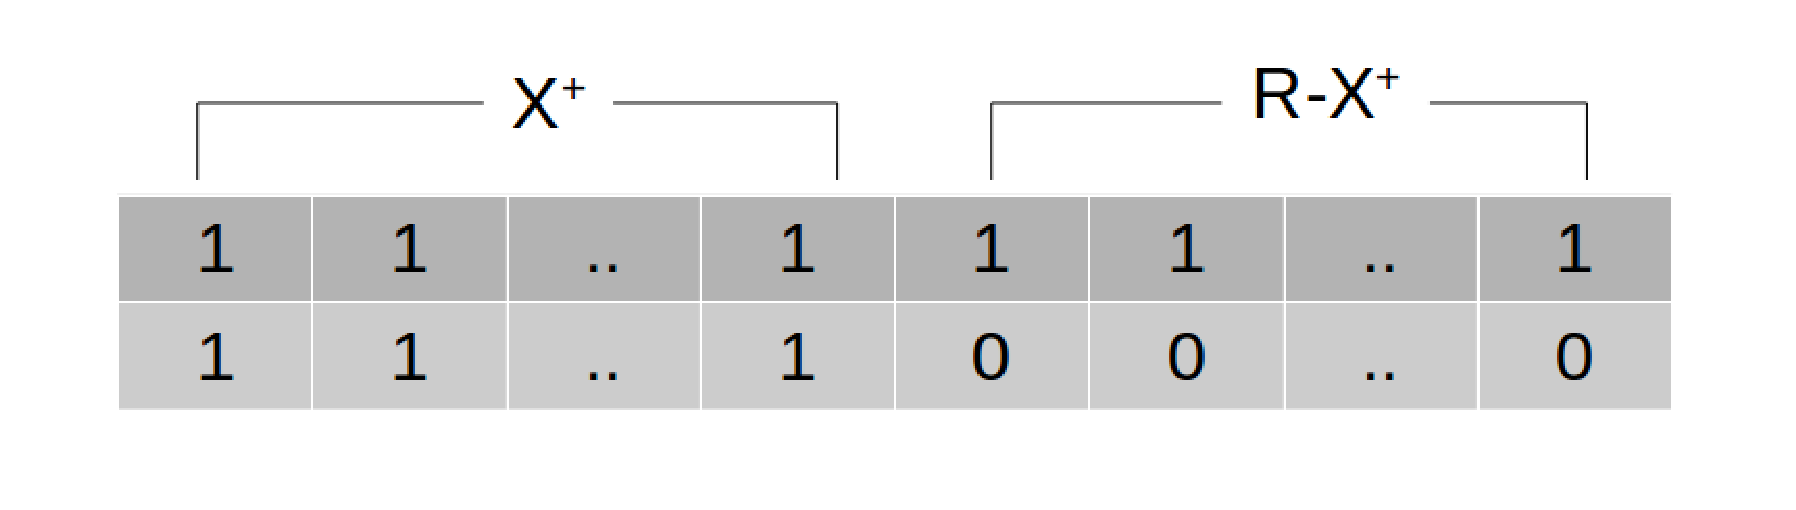
\includegraphics[width=250px]{img_4_4_2.eps} 
\end{center}
Mostriamo che:
\begin{itemize}
 \item $r$ è un'istanza legale di $R$. Sia $V \rightarrow W$ una dipendenza funzionale in $F$ e supponiamo
 per assurdo che non sia soddisfatta da $r$. In tal caso le due tuple di $r$ devono avere gli stessi valori
 per $V$ e differenti valori per $W$; ciò implica che $V \subseteq X^+$ e $W \cap (R-X^+)\not = \emptyset$.
 Poiché $V \subseteq X^+$, per il \linkto{lemma4_1}{Lemma 4.1}, si ha che $X \rightarrow V \in F^A$; pertanto,
 per l'assioma della transitività, $X \rightarrow W \in F^A$ e, quindi, per il Lemma 4.1,
 $W \subseteq X^+$ (che contraddice $W \cap (R-X^+)\not =\emptyset$).
 \item $r$ non soddisfa $X \rightarrow Y$. Supponiamo per assurdo che $r$ soddisfi $X \rightarrow Y$. Poiché 
 $X \subseteq X^+$ (per l'assioma della riflessività), le due tuple di $r$ coincidono sugli attributi $X$ 
 e quindi, poiché $r$ soddisfa $X \rightarrow Y$, devono coincidere anche sugli attributi $Y$. Questo implica
 che $Y \subseteq X^+$ e quindi, per il Lemma 4.1, che $X \rightarrow Y \in F^A$. \hfill $\Box$
\end{itemize}

\subsubsection{Algoritmo per calcolare $X^+$}
Per stabilire se una decomposizione preserva $F^+$, quest'ultimo va calcolato. Tale operazione potrebbe 
tuttavia richiedere tempo esponenziale dipendente da $|F|$; se $F = \{A \rightarrow B_1, A \rightarrow B_2,
\ldots, A \rightarrow B_n\}$, con $|F|=n$, per le regole della decomposizione e dell'unione si ha che 
$F^+ \supseteq \{A \rightarrow Z\ t.c.\ Z \subseteq B_1B_2\ldots B_n\}$ e quindi $|F^+| = 2^n-1$. D'altra parte,
per sapere se una decomposizione preserva le dipendenze, è sufficiente poter decidere se una dipendenza 
funzionale $X \rightarrow Y \in F^+$; ciò può essere fatto calcolando $X^+$ e verificando se $Y \subseteq 
X^+$.\\ 
Il calcolo di $X^+$ può essere fatto mediante il seguente algoritmo polinomiale.
\begin{alg}
\textsc{Input:} uno schema di relazione $R$, un insieme $F$ di dipendenze funzionali su $R$, un sottoinsieme
$X$ di $R$.\\
\textsc{Output:} $X^+_F$ nella variabile $Z$\\\\
\textsc{Begin}\\
$Z\vcentcolon= X$;\\
$S\vcentcolon= \{A\ t.c.\ (Y \rightarrow V \in F) \wedge (A \in V) \wedge (Y \subseteq Z)\}$;\\
\textsc{while} $S \not \subseteq Z$\\
\indent \textsc{begin}\\
\indent $Z\vcentcolon = Z \cup S$;\\
\indent $S\vcentcolon= \{A\ t.c.\ (Y \rightarrow V \in F) \wedge (A \in V) \wedge (Y \subseteq Z)\}$;\\
\indent \textsc{end}\\
\textsc{end}\\
\end{alg}
\begin{exmp}
 Ecco un esempio di esecuzione di tale algoritmo. Sia $R = ABCDEHL$ ed $F=\{A\rightarrow B$, $BC\rightarrow D$,
 $D\rightarrow HL$, $E\rightarrow D\}$. $X=A$.\\\\
 Passo 0: $Z^{(0)}=A$ e $S^{(0)}=B$ \\
 Passo 1: $Z^{(1)}=AB$ mentre $S$ rimane lo stesso.\\
 L'algoritmo termina e $X^+=A^+=AB$.
\end{exmp}

\begin{theo}
L'Algoritmo 4.1 calcola correttamente la chiusura di un insieme di attributi $X$ rispetto ad un insieme $F$ 
di dipendenze funzionali.
\end{theo}
\textbf{Dimostrazione.} Si indichi con $Z^{(0)}$ il valore iniziale di $Z$ (ovvero $Z^{(0)} = X$) e con 
$Z^{(i)}$ ed $S^{(i)}$, $i \geq 1$, i valori di $Z$ ed $S$ dopo l'$i$-esima esecuzione del corpo del ciclo; 
\`e facile vedere che $Z^{(i)} \subseteq Z^{(i+1)}$, $\forall i$. Sia $j$ tale che $S^{(j)} \subseteq Z^{(j)}$
(cio\`e $Z^{(j)}$ \`e il valore di $Z$ quando l'algoritmo termina); si proverà che:
\begin{center}
 \begin{math}
   A \in X^+ \Leftrightarrow A \in Z^{(j)}
 \end{math}
\end{center}
\emph{\textbf{Parte solo se.}} Verrà dimostrato per induzione su $i$ che $Z^{(i)} \subseteq X^+$, $\forall i$, 
e quindi, in particolare $Z^{(j)} \subseteq X^+$.\\
\emph{Base dell'induzione}: $i=0$. Poiché $Z^{(0)} = X$ e $X\subseteq X^+$, si ha $Z^{(0)} \subseteq X^+$.\\
\emph{Induzione}: $i>0$. Per l'ipotesi induttiva $Z^{(i-1)} \subseteq X^+$. Sia $A$ un attributo in $Z^{(i)}
-Z^{(i-1)}$; deve esistere una dipendenza $Y \rightarrow V \in F$ tale che $Y\subseteq Z^{(i-1)}$ e $A \in V$.
Poiché $Y \subseteq Z^{(i-1)}$, per l'ipotesi induttiva si ha che $Y \subseteq X^+$; pertanto, per il 
\linkto{lemma4_1}{Lemma 4.1}, $X \rightarrow Y \in F^A$. Poiché $X \rightarrow Y \in F^A$ e $Y \rightarrow V
\in F$, per l'assioma della transitività si ha $X \rightarrow V \in F^A$ e quindi, per il Lemma 4.1, $V 
\subseteq X^+$. Pertanto, $\forall A \in Z^{(i)} -Z^{(i-1)}$ si ha $A \in X^+$. Da ciò segue, per l'ipotesi 
induttiva, che $Z^{(i)} \subseteq X^+$.\\
\emph{\textbf{Parte se.}} Sia $A$ un attributo in $X^+$. Mostreremo che $A \in Z^{(j)}$. Poiché $A \in X^+$,
si ha $X \rightarrow A \in F^+$ (per il \linkto{teorema4_3}{Teorema 4.3}); pertanto $X \rightarrow A$ deve 
essere soddisfatta da ogni istanza legale di $R$. Si consideri la seguente istanza $r$ di $R$:
\begin{center}
 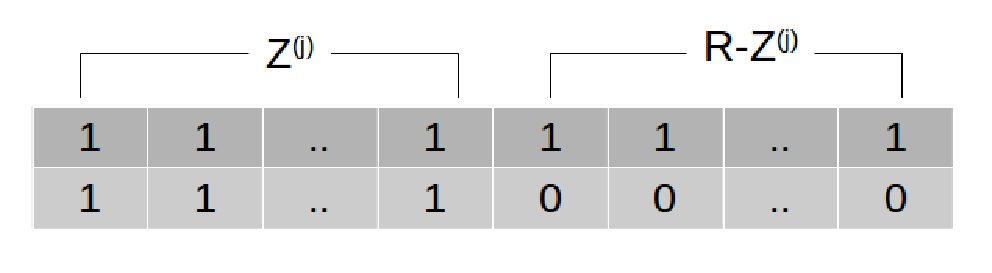
\includegraphics[width=250px]{img_4_4_3.eps}
\end{center}
Mostriamo che $r$ è un'istanza legale di $R$. Infatti, se, per assurdo, esistesse in $F$ una dipendenza
funzionale $V \rightarrow W$ non soddisfatta da $r$, si dovrebbe avere $V \subseteq Z^{(j)}$ e $W \cap 
(R-Z^{(j)})\not = \emptyset$; ma, in tal caso, si avrebbe $S^{(j)} \not \subseteq Z^{(j)}$ (contraddizione).
Poiché $r$ è un'istanza legale di $R$ deve soddisfare $X \rightarrow A$; ma, allora, poiché $X = Z^{(0)} 
\subseteq Z^{(j)}$, $A$ deve essere in $Z^{(j)}$.\hfill $\Box$\\

Tramite l'\textsc{Algoritmo 4.1} possiamo verificare se un insieme di attributi è una chiave valida per
uno schema di relazione; basta verificare, per la sua \linkto{defn_4_3}{Definizione 4.3} e per il \linkto{lemma4_1}{Lemma 4.1},
che la sua chiusura rispetto ad $F$ includa o sia uguale alla relazione e che non lo siano le chiusure
dei suoi sottoinsiemi. Vediamo un esempio.
\begin{exmp}
Sia $R=ABCDEH$ ed $F=\{AB\rightarrow CD$, $C\rightarrow DE$, $E\rightarrow AC\}$. Mostrare che:
\begin{itemize}
 \item $ABH$ è chiave per $R$;
 \item sapendo che è l'unica chiave di $R$, dire perché $R$ non è in 3NF.
\end{itemize}

\noindent \textbf{Soluzione.}\\
$(ABH)^+_F = ABCDEH = R$ e inoltre\\
$(AB)^+_F = ABCDE \not= R$\\
$(AH)^+_F = AH \not= R$\\
$(HB)^+_F = HB \not= R$\\

Ne tantomeno lo saranno le chiusure dei singoli attributi. Quindi abbiamo dimostrato che $ABH$ è chiave di $R$.\\
La relazione $R$ non è in 3NF perché contiene dipendenze parziali e transitive:
\begin{itemize}
 \item $AB\rightarrow CD$ è una dipendenza parziale;
 \item $C\rightarrow DE$, $E\rightarrow AC$ sono dipendenze transitive;
\end{itemize}
e ciò va contro la definizione di schema in Terza Forma Normale.
\end{exmp}


\subsection{Decomposizioni che preservano le dipendenze funzionali}
Si vuole ora formalizzare il concetto di decomposizione che ``preserva un insieme di dipendenze funzionali''.
A tal fine, cominciamo con l'introdurre i concetti di \emph{decomposizione} di uno schema di relazione ed 
\emph{equivalenza} tra due insiemi di dipendenze funzionali.\\
\begin{defn}
Sia $R$ uno schema di relazione. Una \textbf{decomposizione} di $R$ è una famiglia $\rho = \{R_1, R_2, \ldots, 
R_k\}$ di sottoinsiemi di $R$ che \emph{ricopre} $R$ ($\bigcup_{i=1}^k R_i = R$).
\end{defn}
\begin{exmp}
Sia $R = ABC$. Le decomposizioni $\{AB, BC\}$ e $\{A, BC\}$ sono valide, mentre non lo è $\{AB, B\}$ poiché
manca l'attributo $C$.
\end{exmp}

\subsubsection{Equivalenza tra due insiemi di dipendenze funzionali}
\begin{defn}
Siano $F$ e $G$ due insiemi di dipendenze funzionali. $F$ e $G$ sono \textbf{equivalenti}, in simboli $F \equiv 
G$, se $F^+ = G^+$.
\end{defn}
Verificare l'equivalenza di due insiemi $F$ e $G$ di dipendenze funzionali richiede dunque che venga verificata
l'uguaglianza di $F^+$ e $G^+$, cioè che $F^+ \subseteq G^+$ e contemporaneamente $F^+ \supseteq G^+$. Come 
detto in precedenza, calcolare la chiusura di un insieme di dipendenze funzionali può richiedere tempo 
esponenziale. Il seguente lemma ci permette tuttavia di verificare l'equivalenza dei due insiemi di dipendenze
funzionali in tempo polinomiale.
\label{lemma4_2}
\begin{lem}
Siano $F$ e $G$ due insiemi di dipendenze funzionali. $F \subseteq G^+ \Rightarrow F^+ \subseteq G^+$. 
\end{lem}
\textbf{Dimostrazione.} Sia $f \in (F^+ -F)$. Poiché, per il \linkto{teorema4_3}{Teorema 4.3}, $f$ è derivabile
da $F$ mediante gli assiomi di Armstrong e ogni dipendenza funzionale in $F$ è derivabile da $G$ mediante gli 
assiomi di Armstrong, $f$ è derivabile da $G$ mediante gli assiomi di Armstrong. \hfill $\Box$

\begin{defn}
Sia $R$ uno schema di relazione, $F$ un insieme di dipendenze funzionali su $R$ e $\rho = \{R_1, R_2, \ldots,
R_k\}$ una decomposizione di $R$. Diciamo che $\rho$ \emph{preserva} $F$ se $F \equiv \bigcup_{i=1}^k 
\pi_{R_i}(F)$, dove $\pi_{R_i}(F) = \{X \rightarrow Y\ t.c.\ X \rightarrow Y \in F^+ \wedge XY \subseteq R_i\}$.
\end{defn}

\begin{exmp}
 Riprendiamo i dati dell'\linkto{esempio_4_2}{Esempio 4.2}: la relazione $Studente = \{Matr, Com, Prov\}$,
 con $F = $ \{$Matr\rightarrow Com$, $Matr\rightarrow Prov$, $Com\rightarrow Prov$\}. Due decomposizioni possibili
 individuate precendentemente sono:
  \begin{center}
    $R_1 = \{Matr, Com\}$ con $F_1 = \{Matr\rightarrow Com\}$ \\
    $R_2 = \{Matr, Prov\}$ con $F_2 = \{Matr\rightarrow Prov\}$ \\
   \end{center}
 Si verifica applicando la definizione 4.10 che la dipendenza $Com \rightarrow Prov$ non è preservata, 
 perché in $R_1$ manca $Prov$ e in $R_2$ manca $Com$. Una decomposizione alternativa per $R_2$ è
 $\{Com, Prov\}$; in questo modo tutte le dipendenze funzionali sono preservate. In altre parole abbiamo
 \textbf{proiettato le dipendenze}, ovvero abbiamo preso gli attributi $X$ e $Y$ da una dipendenza funzionale
 $X \rightarrow Y$ e vedere se essi sono presenti nella relazione esaminata.
\end{exmp}


\subsubsection{Algoritmo per verificare l'equivalenza tra F e G}
Verificare se una decomposizione preserva un insieme di dipendenze funzionali $F$ richiede, dunque,
che venga verificata l'equivalenza dei due insiemi di dipendenze funzionali $F$ e $G = \bigcup_{i=1}^k
\pi_{R_i}(F)$; poiché, per definizione, $F^+ \supseteq G$, per il \linkto{lemma4_2}{Lemma 4.2} è sufficiente
verificare che $F\subseteq G^+$; ciò può essere fatto con il seguente algoritmo (la cui correttezza è una 
banale conseguenza del \linkto{lemma4_1}{Lemma 4.1} e del \linkto{teorema4_3}{Teorema 4.3}).

\begin{alg}
\textsc{Input:} due insiemi $F$ e $G$ di dipendenze funzionali su $R$;\\
\textsc{Output:} la variabile \emph{successo} che avrà valore \textsc{true} se $F\subseteq G^+$, \textsc{false}
altrimenti;\\
\textsc{Begin}\\
$successo\vcentcolon=\ true$;\\
\textsc{for each} $X \rightarrow Y \in F$\\
\indent \textsc{begin}\\
\indent $calcola\ X_{G}^+$;\\
\indent \textsc{if} $Y \not\subseteq X^+_G$ \textsc{then} $successo=false$;\\
\indent \textsc{end}\\
\textsc{end}\\
\end{alg}

\noindent L'\textsc{Algoritmo 2} richiede che venga calcolato $X^{+}_G$; se si volesse utilizzare a tale scopo l'\textsc{Algoritmo 1}
si dovrebbe prima calcolare $G$, ma, per la definizione di $G$, ciò richiederebbe il calcolo di $F^+$ che
richiede tempo esponenziale. Il seguente algoritmo permette di calcolare $X^{+}_G$ a partire da $F$.

\begin{alg}
\textsc{Input}: uno schema di relazione $R$, un insieme $F$ di dipendenze funzionali su $R$, una
decomposizione $\rho =\{R_1, R_2, \ldots, R_k\}$ di $R$, un sottoinsieme $X$ di $R$;\\
\textsc{Output}: la chiusura di $X$ rispetto a $G = \bigcup_{j=1}^k \pi_{R_j}(F)$, (nella variabile $Z$);\\\\
\textsc{Begin}
$Z\vcentcolon = X$;\\
$S\vcentcolon = \emptyset$;\\
\textsc{for} $j\vcentcolon = 1$ \textsc{to} $k$\\
\indent$S \vcentcolon= S \cup (Z \cap R_j)^{+}_F \cap R_j$;\\
\textsc{while} $S \not\subseteq Z$\\
\indent \textsc{Begin}\\
\indent $Z\vcentcolon = Z \cup S$;\\
\indent \textsc{for} $j\vcentcolon= 1$ \textsc{to} $k$\\
\indent \indent $S\vcentcolon= S \cup (Z \cap R_j)^{+}_F \cap R_j$;\\
\indent \textsc{end}\\
\textsc{end}\\
\end{alg}
\begin{exmp}
Dato $R=ABCDEH$, $F=\{AB\rightarrow CD$, $E \rightarrow H$, $CD\rightarrow E$, $H\rightarrow AB\}$ ed una scomposizione
di $R$, $\rho=\{ABCD$, $CDEH\}$. $\rho$ preserva $F$?\\

\noindent \textbf{Soluzione.}\\
Prendiamo la prima dipendenza funzionale in $F$, $AB\rightarrow CD$. Calcoliamo $(AB)^+_G$.\\\\
$Z^{(0)}= AB$;\\
$S^{(0)} = (AB \cap ABCD)^+_F \cap ABCD = ABCD$;\\
$S^{(1)} = S^{(0)} \cup (AB \cap CDEH)^+_F \cap CDEH = S^{(0)} \cup \emptyset$;\\\\
Dato che $S\subseteq Z$ saltiamo il ciclo \textsc{while} e torniamo all'Algoritmo 1. $CD \subseteq ABCD$ 
quindi la variabile \emph{successo} rimane uguale a \emph{true}; per ogni altra dipendenza seguiamo lo
stesso procedimento. Troveremo quindi che:
\begin{itemize}
 \item $AB\rightarrow CD \in G^+$
 \item $E \rightarrow H  \in G^+$
 \item $CD\rightarrow E \in G^+$
 \item $H\rightarrow AB  \in G^+$
\end{itemize}
quindi $\rho$ preserva $R$.
\end{exmp}

\begin{theo}
Sia $R$ uno schema di relazione, $F$ un insieme di dipendenze funzionali su $R$, $\rho =\{R_1, R_2, \ldots, R_k\}$
una decomposizione di $R$ e $X$ un sottoinsieme di $R$. L'Algoritmo 4.3 calcola correttamente $X^{+}_G$, dove 
$G = \bigcup_{j=1}^k \pi_{R_j}(F)$.
\end{theo}
\textbf{Dimostrazione.} Indichiamo con $Z^{(0)}$ il valore iniziale di $Z$ ($Z^{(0)} = X$) e con $Z^{(i)}$, $i \geq 
1$, il valore di $Z$ dopo l'$i$-esima esecuzione dell'assegnazione $Z \vcentcolon= Z \cup S$; è facile vedere che 
$Z^{(i)} \subseteq Z^{(i+1)}$, $\forall i$. Sia $Z^{(f)}$ il valore di $Z$ quando l'algoritmo termina; proveremo che:
\begin{center}
\begin{math}
  A \in X^{+}_G \Leftrightarrow  A \in Z^{(f)} 
\end{math}
\end{center}
\textbf{\emph{Parte solo se.}} Mostreremo per induzione su $i$ che $Z^{(i)} \subseteq X^{+}_G$, $\forall i$.\\
\emph{Base dell'induzione}: $i=0$. Poiché $Z^{(0)} = X$ e $X \subseteq X^+$, si ha $Z^{(0)} \subseteq X^{+}_G$.\\
\emph{Induzione}: $i >0$. Per l'ipotesi induttiva $Z^{(i-1)} \subseteq X^{+}_G$. Sia $A$ un attributo in $Z^{(i)}
-Z^{(i-1)}$; in tal caso deve esistere un indice $j$ tale che $A \in (Z^{(i-1)} \cap R_j)^{+}_F \cap R_j$. Poiché
$A \in (Z^{(i-1)} \cap R_j)^{+}_F$ si ha $(Z^{(i-1)} \cap R_j) \rightarrow A \in F^+$ (per il Teorema 4.3).\\
Poiché $(Z^{(i-1)} \cap R_j) \rightarrow A \in F^+$, $A \in R_j$ e $Z^{(i-1)} \cap R_j \subseteq R_j$ si ha, per 
la definizione di $G$, che $(Z^{(i-1)} \cap R_j) \rightarrow A \in G$. Poiché per l'ipotesi induttiva si ha che 
$X \rightarrow Z^{(i-1)} \in G^+$, per la regola di decomposizione si ha anche che $X \rightarrow (Z^{(i-1)} 
\cap R_j) \in G^+$ e, quindi, per l'assioma della transitività, che $X \rightarrow A \in G^+$, cioè $A \in X^{+}_G$.
Quindi $Z^{(i)} \subseteq X^{+}_G$.\\
\textbf{\emph{Parte se.}} Mostreremo che $X^{+}_G \subseteq Z^{(f)}$ tenendo conto anche della seguente proposizione:
\begin{prop}
Presi comunque due insiemi di attributi $X$ ed $Y$ e un insieme di dipendenze funzionali $F$ si ha, per la 
definizione di chiusura di un insieme di attributi, $X \subseteq Y \Rightarrow X^{+}_F \subseteq Y^{+}_F$. 
\end{prop}
Poichè $X = Z^{(0)} \subseteq Z^{(f)}$, dalla Proposizione 4.5 segue che $X^{+}_G \subseteq (Z^{(f)})^{+}_G$. 
Mostreremo che $Z^{(f)} = (Z^{(f)})^+_G$ da cui segue $X^+_G \subseteq Z^{(f)}.$\\
Supponiamo per assurdo che $Z^{(f)}\not =(Z^{(f)})^+_G$. Consideriamo l'\textsc{Algoritmo 4.1} che, per evitare ambiguità,
riscriviamo sostituendo la variabile $W$ alla variabile $Z$ e la variabile $U$ alla variabile $S$:\\

\noindent\textsc{Input:} uno schema di relazione $R$, un insieme $F$ di dipendenze funzionali su $R$, un sottoinsieme
$X$ di $R$.\\
\textsc{Output:} $X^+_F$ nella variabile $W$\\\\
\textsc{Begin}\\
$W\vcentcolon= X$;\\
$U\vcentcolon= \{A\ t.c.\ Y \rightarrow V \in F \wedge A \in V \wedge Y \subseteq W\}$;\\
\textsc{while} $U \not \subseteq W$\\
\indent \textsc{begin}\\
\indent $W\vcentcolon = W \cup U$;\\
\indent $U\vcentcolon= \{A\ t.c.\ Y \rightarrow V \in F \wedge A \in V \wedge Y \subseteq W\}$;\\
\indent \textsc{end}\\
\textsc{end}\\

Se eseguiamo tale algoritmo fornendo in input l'insieme di attributi $Z^{(f)}$ e l'insieme di dipendenze 
funzionali $G$, al termine la variabile $W$ conterrà $(Z^{(f)})^+_G$. Se, come abbiamo supposto per assurdo,
$Z^{(f)}\not =(Z^{(f)})^+_G$, deve esistere un attributo $B$ che appartiene a $U^{(0)}$ e non appartiene 
a $W^{(0)} =Z^{(f)}$ (altrimenti si avrebbe $Z^{(f)} =(Z^{(f)})^+_G$). D'altra parte si ha:
\begin{center}
\begin{math}
U^{(0)} = \{A\ t.c.\ Y \rightarrow V \in G \wedge A \in V \wedge Y \subseteq W^{(0)}\}
\end{math}
\end{center}
e quindi, per la definizione di $G$, deve esistere $j$ tale che:
\begin{center}
 \begin{math}
  B \in \{A\ t.c.\ Y \rightarrow V \in F^+ \wedge A \in V \wedge Y \subseteq W^{(0)} \wedge YV \subseteq R_j\}
 \end{math}
\end{center}
Da $Y \subseteq W^{(0)} \wedge YV \subseteq R_j$ segue che:
\begin{center}
 \begin{math}
  [a]\ Y \subseteq W^{(0)} \cap R_j = Z^{(f)} \cap R_j
 \end{math}
\end{center}
Inoltre dal fatto che $Y \rightarrow V \in F^+$ segue, per il \linkto{lemma4_1}{Lemma 4.1}, che $V \subseteq Y^+_F$
e, quindi, per la [a] e per la Proposizione 4.5 si ha che $V \subseteq (Z^{(f)} \cap R_j)^+_F$. Infine 
poichè $YV \subseteq R_j$ si ha:
\begin{center}
 \begin{math}
 V \subseteq (Z^{(f)} \cap R_j)^+_F \cap R_j
 \end{math}
\end{center}
Poiché $B \in V$ si ha che $B \in (Z^{(f)} \cap R_j)^+_F \cap R_j$ e quindi $B \in S^{(f)}$. Poiché $B$ non 
appartiene a $Z^{(f)}$ (per l'ipotesi per assurdo), $Z^{(f)}$ non può essere il valore finale di $Z$ 
(contraddizione). \hfill $\Box$

\subsection{Decomposizioni con Join senza perdita}

Come è stato ribadito nel paragrafo 4.3, se si decompone uno schema di relazione $R$ che non è in 3NF si
vuole che la decomposizione $\{R_1, R_2, \ldots, R_k\}$ ottenuta sia tale che ogni istanza legale $r$
di $R$ sia ricostruibile mediante join naturale (il cui simbolo ricordiamo essere $\bowtie$) da un istanza 
legale $\{r_1, r_2, \ldots, r_k\}$ dello schema decomposto $\{R_1, R_2, \ldots, R_k\}$. Poiché per ricostruire
una tupla $t$ di $r$ è necessario che $t[R_i] \in R_i$, $\forall i \in \{1, \ldots, k\}$, si deve avere $r_i =
\pi_{R_i}(r)$, $\forall i \in \{1, \ldots, k\}$.
\begin{defn}
Sia $R$ uno schema di relazione. Una decomposizione $\rho = \{R_1, R_2, \ldots, R_k\}$ di $R$ ha un
\emph{join senza perdita} se per ogni istanza legale $r$ di $R$ si ha $r = \pi_{R_1}(r) \bowtie \pi_{R_2}(r) 
\bowtie \ldots \bowtie \pi_{R_k}(r)$.
\end{defn}
\begin{theo}
Sia $R$ uno schema di relazione e $\rho = \{R_1, R_2, \ldots, R_k\}$ una decomposizione di $R$. Per ogni
istanza legale $r$ di $R$, indicato con $m_{\rho}(r) =\pi_{R_1}(r) \bowtie \pi_{R_2}(r) 
\bowtie \ldots \bowtie \pi_{R_k}(r)$, si ha:
\begin{enumerate}
 \item $r\subseteq m_{\rho}(r)$
 \item $\pi_{R_i}(m_{\rho}(r)) = \pi_{R_i}(r)$
 \item $m_{\rho}(m_{\rho}(r)) = m_{\rho}(r)$
\end{enumerate}
\end{theo}
\textbf{Dimostrazione.}\\
\emph{Prova di }[1]. Sia $t$ una tupla di $r$. $\forall i \in \{1, \ldots, k\}$, $t[R_i] \in \pi_{R_i}(r)$ e
quindi $t \in m_{\rho}(r)$.\\
\emph{Prova di }[2]. Per il punto [1] si ha $r \subseteq m_{\rho}(r)$ e, quindi, $\pi_{R_i}(r) \subseteq 
\pi_{R_i}(m_{\rho}(r))$. E' sufficiente, pertanto, mostrare che $\pi_{R_i}(r) \supseteq \pi_{R_i}(m_{\rho}(r))$.
Banalmente, per ogni tupla $t \in m_\rho(r)$ e per ogni $i \in \{1, \ldots, k\}$, deve esistere una tupla
$t' \in r\ t.c.\ t[R_i] = t'[R_i]$.\\
\emph{Prova di }[3]. Per il punto [2] si ha $\pi_{R_i}(m_\rho(r)) = \pi_{R_i}(r)$. Pertanto
\begin{center}
$m_\rho(m_\rho(r)) = \pi_{R_1}(m_\rho(r)) \bowtie \ldots \bowtie \pi_{R_k}(m_\phi(r)) = \pi_{R_1}(r) \bowtie
\ldots \bowtie \pi_{R_k}(r) = m_\rho(r)$. 
\end{center}
\hfill $\Box$\\\\
Il seguente algoritmo permette di decidere in tempo polinomiale se una decomposizione di uno schema di relazione
ha un join senza perdita.

\begin{alg}
 \textsc{Input}: uno schema di relazione $R$, un insieme $F$ di dipendenze funzionali su $R$, una decomposizione
 $\rho = \{R_1, R_2, \ldots, R_k\}$ di $R$;\\
 \textsc{Output}: decide se $\rho$ ha un join senza perdita;\\\\
 \textsc{Begin}\\
 Costruisci una tabella $r$ nel modo seguente:
 \begin{itemize}
  \item $r$ ha $|R|$ colonne e $|\rho|$ righe
  \item all'incrocio dell'$i$-esima riga e della $j$-esima colonna si metta:
  \begin{itemize}
   \item il simbolo $a_j$ se l'attributo $A_j \in R_i$;
   \item il simbolo $b_{i,j}$ altrimenti;
  \end{itemize}
 \end{itemize}
 \textsc{repeat}\\
 \indent \textsc{for each} $X\rightarrow Y \in F$\\
 \indent \indent \textsc{do}\\
 \indent \indent \textsc{if} $\exists \{t_1, t_2\} \in r\ t.c.\ t_1[X]=t_2[X] \wedge t_1[Y]\not= t_2[Y]$ \textsc{then}\\
 \indent \indent \indent \textsc{for each} $A_j \in Y$\\
 \indent \indent \indent \indent \textsc{if} $t_1[A_j]=`a_j\text{'}$ \textsc{then} $t_2[A_j]\vcentcolon= t_1[A_j]$;\\
 \indent \indent \indent \indent \textsc{else} $t_1[A_j]\vcentcolon= t_2[A_j]$;\\\\
 \textsc{until} $r$ ha una riga con tutte `a' \textsc{or} $r$ non è cambiato;\\
 \textsc{if} $r$ ha una riga con tutte `a' \textsc{then}\\
 \indent $\rho$ ha un join senza perdita;\\
 \textsc{else}\\
 \indent $\rho$ non ha un join senza perdita;\\
 \textsc{end}\\
\end{alg}

Il seguente esempio mostra come tale algorimo viene applicato.\\
\begin{exmp}
 Sia $R=ABCDE$ uno schema di relazione, $F=\{C\rightarrow D,\ DH\rightarrow C,\ D\rightarrow H,\ A \rightarrow BC\}$
 un insieme di dipendenze funzionali su $R$ e $\rho = \{AE, ABDH, CDE\}$ una scomposizione di $R$. Quello che 
 vogliamo sapere è: $\rho$ ha un join senza perdita?\\
 Come indicato dall'Algoritmo 4.4, si costruisca una tabella che ha come colonne gli attributi di $R$ e come 
 righe le varie relazioni in $\rho$, inserendo poi in ogni cella uno dei due simboli indicati nell'algoritmo,
 secondo il criterio specificato. Nella cella individuata dalla prima colonna e dalla prima riga, ad esempio, 
 va messo il simbolo $a_1$ visto che l'attributo $A$ rappresentante la \emph{prima} colonna è presente nella 
 relazione rappresentante la prima riga; nella seconda colonna, prima riga, la cella contiene $b_{1,2}$ poiché
 $B$ non è presente in $AE$.
 \begin{center}
  \begin{tabular}{c|c|c|c|c|c|c}
    & \textbf{A} & \textbf{B} &\textbf{C}&\textbf{D}&\textbf{E}&\textbf{H}\\
   \hline
   \textbf{AE} & $a_1$ & $b_{1,2}$ & $b_{1,3}$ & $b_{1,4}$ & $a_5$ & $b_{1,6}$\\
   \hline
   \textbf{ABDH}& $a_1$ & $a_2$ & $b_{2,3}$ & $a_4$ & $b_{2,5}$ & $a_6$\\
   \hline
   \textbf{CDE} & $b_{3,1}$ & $b_{3,2}$ & $a_3$ & $a_4$ & $a_5$ & $b_{3,6}$\\
  \end{tabular}
 \end{center}
 
 Ora, per ogni dipendenza funzionale $A\rightarrow Y \in F$, controlliamo se ci sono due righe (tuple) $t_1$
 e $t_2$ tali che $t_1[X] = t_2[X]$ e $t_1[Y] \not= t_2[Y]$. In questo caso abbiamo le dipendenzefunzionali $D\rightarrow H$ e 
 $A \rightarrow BC$ verifica tale condizione; per convenienza conviene segnare, ad ogni iterazione dell'algoritmo, quali 
 dipendenze funzionali verifichino la suddetta condizione. Usiamo la seguente tabella dove le colonne sono le iterazioni, 
 e le righe rappresentano le dipendenze funzionali. Inseriremo una ``$\checkmark$'' quando una dipendenza funzionale 
 verifica la condizione; ``$\cdot$'' altrimenti:\\
 \begin{center}
  \begin{tabular}{l|c|}
   & $I_1$\\
   \hline
   $C\rightarrow D$ & $\cdot$\\
   $DH\rightarrow C$& $\cdot$\\
   $D \rightarrow H$ & $\checkmark$\\
   $A \rightarrow BC$ & $\checkmark$\\
  \end{tabular}
 \end{center}
 
 Tornando alla tabella precedente, visto che l'ultima dipendenza funzionale verifica la condizione cercata nelle righe 1 e 2,
 andiamo a modificare i valori di ogni attributo $Y$, in questo caso $Y= BC$; dato che $t_1[B]\not= a_j$ abbiamo che il valore
 della cella diviene uguale a $t_2[B]$, mentre $t_1[C]\vcentcolon= t_2[C]$. Dopo queste modifiche, al termine della \textbf{prima 
 iterazione} si ha la seguente situazione:
 \begin{multicols}{2}
   \begin{center}
  \begin{tabular}{c|c|c|c|c|c|c}
    & \textbf{A} & \textbf{B} &\textbf{C}&\textbf{D}&\textbf{E}&\textbf{H}\\
   \hline
   \textbf{AE} & $a_1$ & $\mathbf{a_2}$ & $\mathbf{b_{2,3}}$ & $b_{1,4}$ & $a_5$ & $b_{1,6}$\\
   \hline
   \textbf{ABDH}& $a_1$ & $a_2$ & $b_{2,3}$ & $a_4$ & $b_{2,5}$ & $a_6$\\
   \hline
   \textbf{CDE} & $b_{3,1}$ & $b_{3,2}$ & $a_3$ & $a_4$ & $a_5$ & $\mathbf{a_6}$\\
  \end{tabular}
 \end{center}
 
  \begin{center}
  \begin{tabular}{l|c}
   & $I_1$\\
   \hline
   $C\rightarrow D$ & $\cdot$\\
   $DH\rightarrow C$& $\cdot$\\
   $D \rightarrow H$ & $\checkmark$\\
   $A \rightarrow BC$ & $\checkmark$\\
  \end{tabular}
 \end{center}
 \end{multicols}
L'algoritmo non ha terminato la sua esecuzione perché non ha riscontrato una condizione di uscita (una riga con tutte ``a'' o
l'ultima iterazione eseguita non ha apportato nessun cambiamento). Procediamo quindi con le successive iterazioni.\\

\textbf{Iterazione 2}
 \begin{multicols}{2}
   \begin{center}
  \begin{tabular}{c|c|c|c|c|c|c}
    & \textbf{A} & \textbf{B} &\textbf{C}&\textbf{D}&\textbf{E}&\textbf{H}\\
   \hline
   \textbf{AE} & $a_1$ & $a_2$ & $b_{2,3}$ & $\mathbf{a_4}$ & $a_5$ & $b_{1,6}$\\
   \hline
   \textbf{ABDH}& $a_1$ & $a_2$ & $\mathbf{a_3}$ & $a_4$ & $b_{2,5}$ & $a_6$\\
   \hline
   \textbf{CDE} & $b_{3,1}$ & $b_{3,2}$ & $a_3$ & $a_4$ & $a_5$ & $a_6$
  \end{tabular}
 \end{center}
 
  \begin{center}
  \begin{tabular}{l|c|c}
   & $I_1$ & $I_2$\\
   \hline
   $C\rightarrow D$& $\cdot$ & $\checkmark$\\
   $DH\rightarrow C$& $\cdot$& $\checkmark$\\
   $D \rightarrow H$& $\checkmark$ & $\cdot$\\
   $A \rightarrow BC$& $\checkmark$ & $\cdot$
  \end{tabular}
 \end{center}
 \end{multicols}
\textbf{Iterazione 3}
 \begin{multicols}{2}
   \begin{center}
  \begin{tabular}{c|c|c|c|c|c|c}
    & \textbf{A} & \textbf{B} &\textbf{C}&\textbf{D}&\textbf{E}&\textbf{H}\\
   \hline
   \textbf{AE} & $a_1$ & $a_2$ & $\mathbf{a_3}$ & $a_4$ & $a_5$ & $\mathbf{a_6}$\\
   \hline
   \textbf{ABDH}& $a_1$ & $a_2$ & $a_3$ & $a_4$ & $b_{2,5}$ & $a_6$\\
   \hline
   \textbf{CDE} & $b_{3,1}$ & $b_{3,2}$ & $a_3$ & $a_4$ & $a_5$ & $a_6$
  \end{tabular}
 \end{center}
 
  \begin{center}
  \begin{tabular}{l|c|c|c}
   & $I_1$ & $I_2$ & $I_3$\\
   \hline
   $C\rightarrow D$& $\cdot$ & $\checkmark$ & $\cdot$\\
   $DH\rightarrow C$& $\cdot$& $\checkmark$ & $\cdot$\\
   $D \rightarrow H$& $\checkmark$ & $\cdot$ & $\checkmark$\\
   $A \rightarrow BC$& $\checkmark$ & $\cdot$ & $\checkmark$\\
  \end{tabular}
 \end{center}
 \end{multicols}
\noindent Alla fine della terza iterazione ci accorgiamo che la prima riga è composta da soli elementi $a_j$, quindi l'algoritmo
termina indicando che $\rho$ ha un join senza perdita.
 \end{exmp}


\begin{theo}
Sia $R$ uno schema di relazione, $F$ un insieme di dipendenze funzionali su $R$ e $\rho =\{R_1, R_2, \ldots, R_k\}$
una decomposizione di $R$. L'Algoritmo 4.4 decide correttamente se $\rho$ ha un join senza perdita.
\end{theo}
\textbf{Dimostrazione.} Occorre dimostrare che: quando l'algoritmo termina la tabella r ha una tupla con tutte `a' 
$\Leftrightarrow$ $\rho$ ha un join senza perdita. Verrà dimostrata solo la parte ``solo se'' (per uno sketch della 
prova della parte ``se'' consultare il testo di Ullman).\\
\emph{Parte solo se.} Supponiamo per assurdo $\rho$ abbia un join senza perdita e che quando l'algoritmo
termina la tabella $r$ non abbia una tupla con tutte `a'. La tabella $r$ può essere interpretata come
un'istanza legale di $R$ (basta sostituire ai simboli `a' e `b' valori presi dai domini dei corrispondenti
attributi in modo tale che ad uno stesso simbolo venga sostituito lo stesso valore) in quanto
l'algoritmo termina quando non ci sono più violazioni delle dipendenze in $F$. Poiché nessun
simbolo `a' che compare nella tabella costruita inizialmente viene mai modificato dall'algoritmo,
per ogni $i \in \{1, \ldots k\}$, $\pi_{R_i}(r)$ contiene una tupla con tutte `a'; pertanto $m_\rho(r)$ contiene una 
tupla con tutte `a' e, quindi, $m_\rho(r) \not= r$ (contraddizione).
\begin{cor}
Sia $R$ uno schema di relazione, $F$ un insieme di dipendenze funzionali su $R$ e $\rho = \{R_1, R_2\}$
una decomposizione di $R$.
\begin{center}
$(R_1 \cap R_2) \rightarrow (R_1 - R_2) \vee (R_1 \cap R_2) \rightarrow (R_2 -R_1) \Rightarrow \rho$ ha un join senza 
perdita.                            
\end{center}
\end{cor}

\subsection{Decomposizioni in 3NF che conservano la dipendenze funzionali e hanno un join senza perdita}

In questo paragrafo mostreremo che: 
\begin{prop}
Dato uno schema di relazione $R$ e un insieme di dipendenze funzionali $F$ su $R$ esiste sempre una decomposizione
$\rho = \{R_1, R_2, \ldots, R_k\}$ di $R$ tale che:
\begin{itemize}
 \item $\forall i, i \in \{1, \ldots, k\}$, $R_i$ è in 3NF;
 \item preserva $F$;
 \item $\rho$ ha un join senza perdita
\end{itemize}
e che una tale decomposizione può essere calcolata in tempo polinomiale. 
\end{prop}

A tal fine abbiamo bisogno di introdurre il concetto di copertura minimale di un insieme di dipendenze funzionali.
\begin{defn}
Sia $F$ un insieme di dipendenze funzionali. Una \textbf{copertura minimale} di $F$ è un insieme $G$ di dipendenze 
funzionali equivalente ad $F$ tale che:
\begin{enumerate}
 \item per ogni dipendenza funzionale in $G$ la parte destra è un singleton, cioè è costituita da un unico
attributo (ogni attributo nella parte destra è non ridondante);
 \item $\nexists X \rightarrow A \in G\ t.c.\ \exists X' \subseteq X\ t.c.\ G \equiv G - \{X \rightarrow A\} 
 \cup \{X' \rightarrow A\}$ (ogni attributo nella parte sinistra è non ridondante);
 \item $\nexists X \rightarrow A \in G\ t.c.\ G \equiv G - \{X \rightarrow A\}$ (ogni dipendenza è non ridondante). 
\end{enumerate}
\end{defn}
Per ogni insieme di dipendenze funzionali $F$ esiste una copertura minimale che può essere ottenuta in tempo polinomiale
a partire dall'insieme $G$ equivalente ad $F$ in cui per ogni dipendenza funzionale la parte destra è un singleton 
($G$ esiste sempre per la regola della decomposizione)
\begin{itemize}
 \item prima sostituendo ricorsivamente ogni dipendenza funzionale $A_1, \ldots, A_{i-1}, A_i, A_{i+1}, \ldots, A_n 
 \rightarrow A\}$ tale che $G \equiv G - \{A_1, \ldots, A_{i-1}, A_i, A_{i+1}, \ldots, A_n \rightarrow A\} \cup 
 \{A_1, \ldots, A_{i-1}, A_{i+1}, \ldots, A_n \rightarrow A\}$ con la dipendenza funzionale $\{A_1, \ldots, A_{i-1}, A_{i+1},
 \ldots, A_n \rightarrow A\}$
 \item e successivamente eliminando ricorsivamente ogni dipendenza funzionale $X \rightarrow A\ t.c.\ G \equiv G- 
 \{X \rightarrow A\}$.
\end{itemize}

%EXMP%

Il seguente algoritmo, dato uno schema di relazione $R$ e un insieme di dipendenze funzionali $F$ su $R$, che è una 
copertura minimale, permette di calcolare in tempo polinomiale una decomposizione $\rho = \{R_1, R_2, \ldots, R_k\}$ 
di $R$ tale che:
\begin{itemize}
 \item $\forall i \in \{1, \ldots, k\}$, $R_i$ è in 3NF;
 \item $\rho$ preserva $F$.
\end{itemize}

\begin{alg}
 \textsc{Input}: uno schema di relazione $R$ e un insieme $F$ di dipendenze funzionali su $R$, che è una copertura
 minimale;\\
 \textsc{Output}: una decomposizione $\rho$ di $R$ che preserva $F$ e tale che per ogni schema di relazione in è 
 in 3NF;\\\\
 \textsc{begin}\\
 $S\vcentcolon= \emptyset$;\\
 \textsc{for each} $A \in R$ tale che $A$ non è coinvolto in nessuna dipendenza funzionale in $F$ \textsc{do}\\
 \indent $S\vcentcolon= S \cup \{A\}$;\\
 \textsc{if} $S \not= \emptyset$ \textsc{then}\\
\indent \textsc{begin}\\
\indent $R\vcentcolon= R-S$;\\
\indent $\rho\vcentcolon=\rho \cup \{S\}$;\\
\indent \textsc{end}\\
\textsc{if} esiste una dipendenza funzionale in $F$ che coinvolge tutti gli attributi in $R$ \textsc{then}\\
\indent $\rho\vcentcolon= \rho \cup \{R\}$;\\
\textsc{else}\\
\indent \textsc{for each} $X \rightarrow A \in F$ \textsc{do} $\rho\vcentcolon= \rho \cup \{XA\}$\\
\textsc{end}\\
\end{alg}

\begin{theo}
Sia $R$ uno schema di relazione ed $F$ un insieme di dipendenze funzionali su $R$, che è una copertura minimale. 
L'Algoritmo 4.5 permette di calcolare in tempo polinomiale una decomposizione $\rho$ di $R$ tale che:
\begin{enumerate}
 \item ogni schema di relazione in $\rho$ è in 3NF
 \item preserva $F$.
\end{enumerate}
\end{theo}
\textbf{Dimostrazione.}\\
\emph{$\rho$ preserva $F$.} Sia $G = \bigcup_{i=1}^k \pi_{R_i}(F)$. Poiché per ogni dipendenza funzionale $X 
\rightarrow A \in F$ si ha che $XA \in \rho$, si ha che $G \supseteq F$ e, quindi $G^+ \supseteq F^+$. 
L'inclusione $G^+ \subseteq F^+$ è banalmente verificata in quanto per definizione, $G\subseteq F?+$. \\
\emph{Ogni schema di relazione in $\rho$ è in 3NF.}
Se $S \in \rho$, ogni attributo in $S$ fa parte della chiave e quindi, banalmente, $S$ è in 3NF. Se $R \in \rho$
esiste una dipendenza funzionale in $F$ che coinvolge tutti gli attributi in $R$. Poiché $F$ è una copertura minimale
tale dipendenza avrà la forma $R-A \rightarrow A$; poiché $F$ è una copertura minimale, non ci può essere una 
dipendenza funzionale $X \rightarrow A \in F^+\ t.c.\ X \subset R-A$ e, quindi, $R-A$ è chiave in $R$.
Sia $Y \rightarrow B$ una qualsiasi dipendenza in $F^+$; se $B = A$ allora, poiché $F$ è una copertura minimale, 
$Y = R-A$ (cioè, $Y$ è una superchiave); se $B \not= A$ allora $B \in R-A$ e quindi $B$ è primo.
Se $XA \in \rho$, poiché $F$ è una copertura minimale, non ci può essere una dipendenza funzionale $X' \rightarrow A 
\in F^+\ t.c.\ X' \subset X$ e, quindi, $X$ è chiave in $XA$. Sia $Y \rightarrow B$ una qualsiasi dipendenza in $F^+$ 
tale che $YB \subseteq XA$; se $B = A$ allora, poiché $F$ è una copertura minimale, $Y = X$ (cioè, $Y$ è una 
superchiave); se $B \not= A$ allora $B \in X$ e quindi $B$ è primo.

\begin{theo}
Sia $R$ uno schema di relazione, $F$ un insieme di dipendenze funzionali su $R$, che è una copertura minimale e $\rho$
la decomposizione di $R$ prodotta dall'Algoritmo 4.5. La decomposizione $\sigma = \rho \cup \{K\}$, dove $K$ è una 
chiave per $R$, è tale che:
\begin{enumerate}
 \item ogni schema di relazione in $\sigma$ è in 3NF
 \item $\sigma$ preserva $F$
 \item $\sigma$ ha un join senza perdita. 
\end{enumerate}
\end{theo}
\textbf{Dimostrazione.}\\
\emph{$\sigma$ preserva $F$}. Sia $\sigma =\{R_1, R_2, \ldots, R_k, R_{k+1}\}$ dove $\rho=\{R_1, R_2, \ldots, R_k\}$ 
è la decomposizione ottenuta mediante l'Algoritmo 4.5 e $R_{k+1} = K$. Sia $G'= \bigcup_{i=1}^{k+1}\{X\rightarrow Y 
\in F^+\ t.c.\ XY \in R_i\}$. Poiché per il Teorema 4.8 $F\equiv G$, dove $G = \bigcup_{i=1}^k \{X\rightarrow Y\in F^+
\ t.c.\ XY\in R_i\}$, è sufficiente dimostrare che $G\equiv G'$, cioè, per il \linkto{lemma4_2}{Lemma 2}, che 
$G\subseteq (G')^+$ e $G'\subseteq G^+$. Infatti, $G\subseteq G'$ e quindi $G\subseteq (G')^+$. Inoltre, per 
definizione, $G' \subseteq F^+$; poiché $F^+ =G^+$, si ha che $G'\subseteq G^+$.\\
\emph{Ogni schema di relazione in $\sigma$ è in 3NF}. Poiché $\sigma =\rho \cup \{K\}$, è sufficiente verificare che 
lo schema di relazione $K$ è in 3NF. Mostriamo che $K$ è chiave per lo schema $K$. Supponiamo per assurdo che
$K$ non sia chiave per lo schema $K$; allora esiste un sottoinsieme proprio $K' \subset K$ tale che $K'\rightarrow 
K \in F^+$; poiché $K$ è chiave per lo schema $R$, $K\rightarrow R \in F^+$; pertanto per transitività $K'\rightarrow
R \in F^+$, che contraddice il fatto che $K$ è chiave per lo schema $R$. Pertanto, è chiave per lo schema $K$ e quindi per
ogni dipendenza funzionale $X \rightarrow A \in F^+$ con $XA \subseteq K$, $A$ è primo.\\
\emph{$\sigma$ ha un join senza perdita.} Supponiamo che l'ordine in cui gli attributi in $R-K$ vengono aggiunti a
$Z$ dall'Algoritmo 4.1 quando calcola $K^+$ sia $A_1, A_2, \ldots, A_n$, e supponiamo che per ogni $i \in 
\{1, \ldots, n\}$, l'attributo $A_i$ venga aggiunto a $Z$ a causa della presenza in $F$ della dipendenza $Y_i 
\rightarrow A_i$ dove 
\begin{center}
$Y_i \rightarrow Z^{(i-1)} = KA_1A_2\ldots A_{i-1} \subseteq K^+$. 
\end{center}

Per dimostrare che $\rho$ ha un join senza perdita mostreremo che quando l'Algoritmo 4.4 è applicato a $\rho$
viene prodotta una tabella che ha una riga con tutte `a'. Senza perdita di generalità, supponiamo che l'Algoritmo 4.4
esamini le dipendenze funzionali $Y_1 \rightarrow A_1, Y_2 \rightarrow A_2, \ldots, Y_n \rightarrow A_n$ in questo ordine.
Dimostreremo per induzione su $i$ che dopo che è stata considerata la dipendenza funzionale $Y_i \rightarrow A_i$ nella 
riga che corrisponde allo schema di relazione $K$ c'è una `a' in ogni colonna $j$ con $j \leq i$.\\
\emph{Base dell'induzione}: $i=1$. Poiché $Y_1 \subseteq Z^{(0)} = K$, sia nella riga che corrisponde allo schema di
relazione $Y_1A_1$ che in quella che corrisponde allo schema di relazione $K$ ci sono tutte `a' in corrispondenza
agli attributi in $Y_1$; inoltre nella riga che corrisponde allo schema di relazione $Y_1A_1$ c'è una `a' in
corrispondenza ad $A_1$. Pertanto l'Algoritmo 4.4 pone una `a' in corrispondenza ad $A_1$ nella riga che corrisponde 
allo schema di relazione $K$.\\ 
\emph{Induzione}: $i > 1$. Per l'ipotesi induttiva, nella riga che corrisponde allo schema di relazione $K$ c'è una
`a' in corrispondenza ad ogni attributo $A_j$ con $j \leq i-1$. Poiché $Y_i \subseteq KA_1A_2\ldots A_{i-1}$, sia nella
riga che corrisponde allo schema di relazione $Y_iA_i$ che in quella che corrisponde allo schema di relazione $K$ ci sono
tutte `a' in corrispondenza agli attributi in $Y_i$; inoltre nella riga che corrisponde allo schema di relazione $Y_iA_i$
c'è una `a' in corrispondenza ad $A_i$. Pertanto l'Algoritmo 4.4 pone una `a' in corrispondenza ad $A_i$ nella riga che 
corrisponde allo schema di relazione $K$.\hfill $\Box$
\subsection{La forma normale di Boyce-Codd}
\textsc{Attenzione!} \emph{Questo paragrafo non è stato trattato nel corso relativo all'anno 2014/2015}.\\

\noindent Successivamente alla terza forma normale sono state definite altre forme normali per gli schemi di relazione, alcune delle 
quali sono basate su vincoli (dipendenze multivalore e dipendenze di join) più generali delle dipendenze funzionali. Una 
forma normale che ancora si basa sul concetto di dipendenza funzionale è la cosidetta forma normale di Boyce-Codd.

\begin{defn}
Siano $R$ uno schema di relazione e $F$ un insieme di dipendenze funzionali su $R$. $R$ è in forma normale di Boyce-Codd 
se per ogni dipendenza funzionale $X \rightarrow A \in F^+$ tale che $A \not\in X$ si ha che $X$ è una superchiave.
\end{defn}
Come è evidente dalla definizione, la forma normale di Boyce-Codd è più restrittiva della terza forma normale: ogni schema 
di relazione in forma normale di Boyce-Codd è in terza forma normale, ma non è vero il viceversa. Infatti, consideriamo 
il seguente schema di relazione, 
\begin{center}
\emph{Orario\_lezioni = $\{$Aula, Giorno, Ora, Corso$\}$}                      
\end{center}
su cui sono definite le seguenti dipendenze funzionali 
\begin{center}
$Aula \rightarrow Giorno$, $Ora \rightarrow Corso$ (in una certa aula in un certo giorno ad una certa
ora viene tenuto un solo corso)  
\end{center}
\begin{center}
$Corso \rightarrow Aula$ (un corso viene tenuto sempre nella stessa aula).
\end{center}
Poiché la chiave di $Orario\_lezioni$ è $\{Aula\ Giorno\ Ora\}$, nella dipendenza funzionale $Corso \rightarrow Aula$ la
parte sinistra non è una superchiave e, quindi, lo schema di relazione $Orario\_lezioni$ non è in forma normale di 
Boyce-Codd pur essendo in terza forma normale. In uno schema che non è in forma normale di Boyce-Codd si presenta ancora 
il problema della ridondanza nella rappresentazione dei dati (ad esempio in $Orario\_lezioni$ il fatto che un corso si 
tiene in una certa aula è ripetuto per ogni ora in cui il corso viene tenuto). Sorge quindi il problema di capire se per
la forma normale di Boyce-Codd valgono risultati analoghi a quelli visti nei paragrafi precedenti per la terza forma
normale, vale a dire se è valida la seguente affermazione:\\

``Dato uno schema di relazione $R$ e un insieme di dipendenze funzionali $F$ su $R$ esiste sempre una decomposizione 
$\rho=\{R_1, R_2, \ldots, R_k\}$ di $R$ tale che:
\begin{itemize}
 \item $\forall i \in \{1, \ldots n\}$, $R_i$ è in forma normale di Boyce-Codd
 \item $\rho$ preserva $F$
 \item ha un join senza perdita''
\end{itemize}

La risposta a questa domanda è negativa. Infatti, è evidente che qualsiasi decomposizione di $Orario\_lezioni$ che non 
contenga lo schema di relazione $\{Aula\ Giorno\ Ora\ Corso\}$, non permette di rappresentare la dipendenza funzionale
$\{Aula\ Giorno\ Ora\} \rightarrow Corso$. Tuttavia è possibile dimostrare che dato uno schema di relazione $R$ e un 
insieme di dipendenze funzionali F su R esiste sempre una decomposizione $\rho=\{R_1, R_2, \ldots, R_k\}$ di $R$ tale 
che:
\begin{itemize}
 \item $\forall i \in \{1, \ldots k\}$, $R_i$ è in forma normale di Boyce-Codd
 \item $\rho$ ha un join senza perdita
\end{itemize}
e che esiste un algoritmo che produce una tale decomposizione in tempo polinomiale. Tale algoritmo fornirebbe nel caso 
dell'esempio esaminato la decomposizione: $\{R_1 =\ Aula\ Corso, R_2 =\ Giorno\ Ora\ Corso\}$.
\newpage
\section{Organizzazione fisica della base di dati}

Un requisito fondamentale di un database è l'efficienza, cioè la capacità di rispondere alle 
richieste dell'utente il più rapidamente possibile: questo obiettivo può essere raggiunto grazie
ad una particolare organizzazione fisica dei dati. In questo capitolo verrà mostrato come il database
è organizzato a livello fisico, ovvero come questo viene salvato sull'unità di memoria 
di massa (disco rigido); nel prossimo paragrafo sarà quindi necessario illustrare brevemente come il
sistema operativo gestisce la lettura e scrittura di tale dispositivo.

\subsection{La memoria secondaria}
Il computer necessita di una \emph{memoria secondaria} dove poter salvare in modo permanente
i dati presenti nella RAM. Questa memoria secondaria è tipicamente un disco rigido, la cui struttura
meccanica è illustrata nella seguente figura.
\begin{center}
 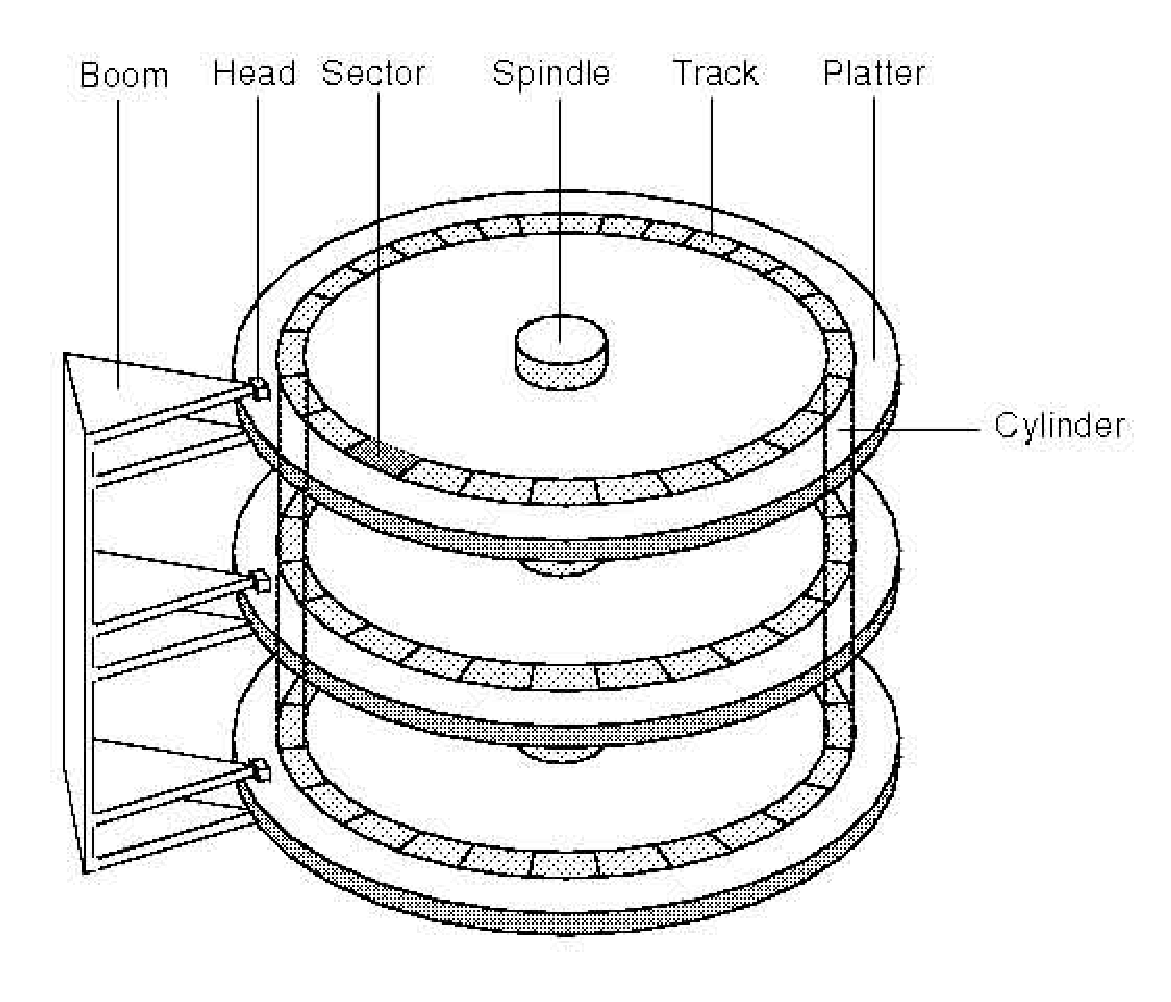
\includegraphics[width=300px]{img_5_1.eps}
\end{center}
L'unità di memoria è composta da più \textbf{piatti}, di solito tre, ognuno dei quali è suddiviso
in \textbf{tracce}: esse sono come cerchi concentrici che partizionano tutta la superficie del
piatto. Al momento della \emph{formattazione}, durante la quale viede data una struttura logica per 
poter memorizzare i dati, impostando la struttura del filesystem che vi verrà creato sopra, vengono
creati i \textbf{settori} (o \textbf{blocchi} o pagine) di dimensione fissa, che varia da $2^9$ a $2^{12}$
bytes.\\
Quando si parla di \emph{accesso} al disco s'intende il trasferimento di un blocco da memoria secondaria 
a memoria principale, quindi \textbf{lettura} di un blocco, o da memoria principale a memoria secondaria, 
ossia \textbf{scrittura} di un blocco. Il tempo necessario per un accesso è dato dalla somma di:
\begin{itemize}
 \item \emph{tempo di posizionamento} della testina sulla traccia in cui si trova il blocco;
 \item \emph{ritardo della rotazione}, necessaria per posizionare la testina all'inizio del blocco;
 \item \emph{tempo di trasferimento} dei dati contenuti nel blocco.
\end{itemize}
Il tempo richiesto per un accesso a memoria secondaria è dell'ordine dei millisecondi, quindi 
notevolmente superiore a quello di elaborazione dei dati in memoria principale. Per questo motivo il 
\textbf{costo} di un'operazione sulla base di dati è definito in termini di \emph{numero di accessi}.

\subsection{Memorizzare le relazioni}

\subsubsection{Record}
Ad ogni relazione corrisponde un file di record che sono tutti dello stesso tipo (numero e 
tipo dei campi): ad ogni attributo corrisponde un \emph{campo}, che è di tipo elementare (interi,
reali, stringhe di caratteri), ed ad ogni tupla corrisponde un record. In un record, oltre ai campi 
che corrispondono agli attributi, ci possono essere altri campi che contengono informazioni sul 
record stesso o puntatori ad altri record.\\
Un \textbf{puntatore} ad un record è essenzialmente un dato che permette di accedere rapidamente a quel
record. Pertanto un puntatore può essere l'indirizzo dell'inizio (primo byte) del record su disco.
Tale scelta però può non essere adeguata se si vuole avere una certa libertà di muovere il record; in
questo caso è preferibile assumere come puntatore una coppia $(b, k)$ in cui $b$ è l'indirizzo del blocco
che contiene il record e $k$ è il valore di uno o più campi che servono come chiave nel file a cui il
record appartiene. In tal modo è possibile spostare il record all'interno del blocco. All'inizio di un 
record alcuni byte possono essere utilizzati per:
\begin{itemize}
 \item specificare il tipo del record, necessario quando in uno stesso blocco sono memorizzati 
 record di tipo diverso;
 \item specificare la lunghezza del record, se esso ha campi a lunghezza variabile;
 \item contenere un bit di ``cancellazione'', utile nel caso che il record sia puntato. In tal caso 
 lo spazio occupato dal record cancellato non può essere riutilizzato
 \item contenere un bit di ``usato/non usato'' per specificare se in quello spazio c'è un record oppure
 è vuoto (contiene valori casuali).
\end{itemize}

Per poter accedere ad un campo di un record contenente un dato è necessario sapere qual è il primo
byte del campo nel record. Se tutti i campi del record hanno lunghezza fissa, basta ordinarli; infatti,
una volta ordinati, l'inizio di ciascun campo sarà sempre ad un numero fisso di byte dall'inizio del
record: il numero di byte del record che precedono il campo è detto \textbf{offset} del campo. Se il record
contiene campi a lunghezza variabile allora l'offset di un campo può variare da un record all'altro.
In tal caso si possono usare due strategie:
\begin{itemize}
 \item all'inizio di ogni campo c'è un contatore che specifica la lunghezza del campo in numero di
byte
\item all'inizio del record ci sono gli offset di ciascun campo a lunghezza variabile (tutti i campi 
a lunghezza fissa precedono quelli a lunghezza variabile).
\end{itemize}

Nel primo caso per individuare la posizione di un campo bisogna esaminare i campi precedenti per
vedere quanto sono lunghi; quindi la prima strategia è meno efficiente della seconda. 

\subsubsection{Blocchi}
I record sono memorizzati nei blocchi. Analogamente a quanto accade per un record, anche in un blocco 
può essere riservato spazio per memorizzare informazioni sul blocco stesso (record cancellati, record 
non usati, puntatori a record se il blocco contiene record a lunghezza variabile), dello spazio 
``sprecato'' (per far in modo che gli offset di campi interi siano multipli di 4) o per collegarlo ad altri 
blocchi in una lista. Se un blocco contiene solo record di lunghezza fissa allora il blocco può essere 
suddiviso in aree (sottoblocchi) di lunghezza fissa ciascuna delle quali può contenere un record. Quando 
bisogna inserire un record nel blocco si cerca un area non usata; se il bit ``usato/non usato'' è in ciascun record
ciò può richiedere la scansione di tutto il blocco; per evitare ciò si possono raccogliere tutti i bit
``usato/non usato'' in uno o più byte all'inizio del blocco. 
In un blocco ci possono essere informazioni sul blocco stesso o puntatori ad altri blocchi.\\

Se un blocco contiene record di lunghezza variabile per accedere ai record si possono usare due
strategie:
\begin{itemize}
 \item si suppone che il primo record abbia inizio dal primo byte del blocco; si pone in ogni record un
campo che ne specifica la lunghezza in termini di numero di byte. Per calcolare il byte di inizio
di un record si somma all'offset del record precedente la sua lunghezza (ed eventualmente si
prende il successivo multiplo di 4);
 \item si pone all'inizio del blocco una \textbf{directory} contenente i puntatori ai record nel blocco 
 (in questo caso un puntatore è l'offset del record nel blocco). Poiché il numero di record che possono
entrare in un blocco è in questo caso variabile, la directory può essere realizzata in uno dei modi
seguenti:
\begin{itemize}
 \item la directory è preceduta da un campo che specifica quanti sono i puntatori nella directory
 \item la directory ha dimensione fissa (può contenere un numero fisso di puntatori) e contiene il
valore 0 (che non può essere un offset) negli spazi che non contengono puntatori (se il
numero di records nel blocco è inferiore al numero di puntatori che possono essere
memorizzati nella directory
\item la directory è una lista di puntatori (la fine della lista è specificata da uno 0).
\end{itemize}
\end{itemize}
L'uso di una directory all'inizio del blocco permette di spostare i record ``puntati''; infatti, basta 
far in modo che il puntatore invece di puntare al record punti al campo della directory che contiene
l'offset. Inoltre permette di spostare i bit di cancellazione dai record alla directory e quindi di
riutilizzare lo spazio occupato da un record a lunghezza variabile quando questo viene cancellato.

\subsection{File}
In questo paragrafo esamineremo diversi tipi di organizzazione fisica di file che consentono la
ricerca di record in base al valore di uno o più campi \emph{chiave}. Il termine ``chiave'' non va inteso nel
senso in cui viene usato nella teoria relazionale, in quanto un valore della chiave non necessariamente 
identifica univocamente un record nel file.
Le operazioni elementari su questi tipi di file sono dunque:
\begin{itemize}
 \item la ricerca di uno o più record con un dato valore per chiave;
 \item l'inserimento di un record con un dato valore per chiave;
 \item la cancellazione di uno o più record con un dato valore per chiave;
 \item la modifica di uno o più record con un dato valore per chiave. 
\end{itemize}

\subsubsection{Heap}
In questo tipo di organizzazione i record sono memorizzati nei blocchi senza alcun ordine: un
record viene sempre inserito come ultimo record del file. L'accesso al file avviene attraverso una
directory che contiene i puntatori ai blocchi; se le dimensioni lo consentono, tale directory può
essere mantenuta in memoria principale durante l'utilizzo del file; altrimenti saranno necessari
ulteriori accessi per portare in memoria principale i necessari blocchi della directory.
Denotiamo con $b$ il numero di blocchi del file ed esprimiamo in termini di $b$ il costo delle varie
operazioni, nella ipotesi che la directory si trovi in memoria principale.
Se la chiave di \textbi{ricerca} non identifica univocamente un record nel file, poiché non esiste alcun
particolare ordinamento dei record, per effettuare una ricerca occorre scandire tutto il file
sequenzialmente e, quindi, il costo di una ricerca è dato da $b$. L'\textbi{inserimento} di un record richiede la
lettura dell'ultimo blocco del file; se in tale blocco c'è spazio sufficiente per memorizzare il nuovo
record, il record viene inserito, altrimenti viene chiesto un nuovo blocco al file system; dopo
l'inserimento del record nel blocco, il blocco deve essere scritto su memoria secondaria. Quindi due
accessi (uno per lettura e uno per scrittura) sono sufficienti per l'inserimento di un record. La
\textbi{cancellazione} di tutti i record con un dato valore per la chiave richiede $b$ accessi in lettura 
per la ricerca di tutti i record che hanno quel valore per la chiave e $c$ accessi in scrittura, dove $c$ è il
numero di blocchi contenenti record con quel valore per la chiave; ulteriori accessi possono essere
necessari se si vuole recuperare lo spazio occupato dai record cancellati trasferendovi record che si
trovano nell'ultimo blocco. La \textbi{modifica} di tutti i record con un dato valore per la chiave richiede $b$
accessi in lettura per la ricerca di tutti i record che hanno quel valore per la chiave e $c$ accessi in
scrittura, dove $c$ è il numero di blocchi contenenti record con quel valore per la chiave.\\\\
Se la chiave di ricerca identifica univocamente un record nel file, la ricerca di un record con un dato
valore per la chiave richiede in media $[b/2]$ accessi. Per ottenere il costo medio occorre sommare i costi 
per accedere ai singoli record e quindi dividere tale somma per il numero dei record. Infatti, per la 
ricerca di un record che si trova nell'$i$-esimo blocco sono necessari $i$ accessi (in lettura); 
pertanto se denotiamo con $n$ il numero di record nel file e con $B$ il numero di record che possono 
essere memorizzati in un blocco ($[n/B]=b$), il numero medio di accessi necessari per la ricerca di un 
record è data da
\begin{center}
$\dfrac{B(1+2+\ldots +b)}{n} = \dfrac{Bb(b+1)}{2n} \simeq [b/2]$ 
\end{center}
(si osservi che $b/2\leq[b/2] \leq (b+1)/2$).\\
L'inserimento di un record richiede la lettura dell'ultimo blocco del file; se in tale blocco c'è spazio
sufficiente per memorizzare il nuovo record, il record viene inserito, altrimenti viene chiesto un
nuovo blocco al file system; dopo l'inserimento del record nel blocco, il blocco deve essere scritto
su memoria secondaria. Quindi 2 accessi (uno per lettura e uno per scrittura) sono sufficienti per
l'inserimento di un record. La cancellazione di un record con un dato valore per la chiave richiede
$[b/2]$ accessi in lettura per la ricerca del record che ha quel valore per la chiave e 1 accesso in
scrittura. Se si vuole recuperare lo spazio occupato dal record cancellato e i record hanno lunghezza
fissa si può trasferire un record che si trova nell'ultimo blocco (restituendo al sistema il blocco se
non vi sono altri record, in modo di ridurre i costi delle successive operazioni sul file) al posto di
quello cancellato. Se si vuole recuperare lo spazio occupato dal record cancellato e i record hanno
lunghezza variabile, si possono far slittare i record nel blocco (aggiornando i puntatori ai record
nell'intestazione del blocco) e, se in tal modo si è ottenuto uno spazio sufficiente per trasferirvi un
record che si trova nell'ultimo blocco, procedere come nel caso precedente. La modifica di un
record con un dato valore per la chiave richiede $[b/2]$ accessi in lettura per la ricerca del record che
ha quel valore per la chiave e 1 accesso in scrittura.\\

\subsubsection{File hash}
In questo tipo di organizzazione i record sono ripartiti in \textbf{bucket} (secchi) in base al valore della
chiave. Se $B$ è il numero dei bucket, questi vengono numerati da $1$ a $B$. Dato un valore $v$ per
chiave il numero del bucket in cui deve trovarsi un record con chiave $v$ è calcolato mediante una
funzione che prende il nome di \emph{funzione hash}.
Ciascun bucket è costituito da uno o più blocchi (come vedremo, affinchè la gestione del file sia
efficiente è opportuno che il numero dei blocchi in un bucket sia piccolo) ed è organizzato come un
heap. L'accesso ai bucket avviene attraverso la bucket directory che contiene $B$ elementi
(normalmente $B$ è sufficientemente piccolo da consentire di mantenere la bucket directory in
memoria principale durante l'utilizzo del file); l'$i$-esimo elemento contiene l'indirizzo (bucket
header) del primo blocco dell'$i$-esimo bucket. Tutti i blocchi di un bucket sono collegati tra loro
mediante puntatori in una lista.
Una funzione hash per essere ``buona'' deve ripartire uniformemente i record nei bucket, cioè al
variare del valore della chiave deve assumere con la ``stessa'' probabilità uno dei valori compresi tra
$0$ e $B-1$. Esiste un'ampia letteratura sulle funzioni hash. In genere, una funzione hash trasforma la
chiave in un intero, divide questo intero per $B$, e fornisce il resto della divisione come numero di
bucket in cui deve trovarsi il record con quel valore della chiave. Una strategia per definire una
funzione hash è, ad esempio, la seguente:
\begin{enumerate}
 \item trattare il valore v della chiave come una sequenza di bit
 \item suddividere tale sequenza in gruppi di bit di uguale lunghezza
 \item sommare tali gruppi trattandoli come interi
 \item dividere il risultato per il numero dei bucket (cioè per $B$)
 \item prendere il resto della divisione come numero del bucket in cui deve trovarsi un record con
chiave $v$.
\end{enumerate}

Una qualsiasi operazione (ricerca, inserimento, cancellazione, modifica) su un file hash richiede la
valutazione di $h(v)$ (dove $v$ è un valore per la chiave e $h$ è la funzione hash) per individuare il bucket
in cui deve trovarsi il record con chiave $v$; successivamente, l'operazione (ricerca, inserimento,
cancellazione, modifica) viene effettuata sul bucket che, come già detto, è organizzato come un
heap. Se la funzione hash distribuisce uniformemente i record nei bucket, ogni bucket è costituito
da un numero di blocchi che è $1/B$-esimo del numero di blocchi di cui è costituito l'intero file.
Pertanto il costo richiesto per un'operazione è approssimativamente $1/B$-esimo del costo che
sarebbe richiesto per fare la stessa operazione se il file fosse organizzato come un heap. Si osservi
che, poiché l'inserimento di un record viene effettuato sull'ultimo blocco del bucket, è opportuno
che la bucket directory contenga anche, per ogni bucket, un puntatore all'ultimo record del bucket.
Da quanto detto appare evidente che quanti più sono i bucket tanto più basso è il costo di ogni
operazione. D'altra parte limitazioni al numero dei bucket derivano dalle seguenti considerazioni:
\begin{enumerate}
 \item ogni bucket deve avere almeno un blocco
\item se le dimensioni della bucket directory sono tali che non può essere mantenuta in memoria
principale durante l'utilizzo del file, ulteriori accessi sono necessari per leggere i blocchi della
bucket directory.
\end{enumerate}

\subsubsection{File con indice (indice sparso)}
Nella presentazione di questo tipo di organizzazione, spesso chiamato \emph{ISAM} (Indexed Sequential
Access Method), assumeremo che il valore della chiave identifica univocamente un record del file.
Inoltre, inizialmente, assumeremo che i record non siano puntati.\\\\
Inizialmente il file viene ordinato in base al valore (crescente) della chiave e viene memorizzato
lasciando in ogni blocco una certa percentuale (ad esempio il 20\%) di spazio non utilizzato per
l'inserimento di nuovi record; quindi viene creato un nuovo file, il \textbf{file indice} che
contiene un record per ogni blocco del file principale, e infine la directory del file indice che 
generalmente ha dimensioni tali da poter essere mantenuta in memoria principale durante l'utilizzo del file.\\
Un file indice è un file i cui record consistono di coppie del tipo $(v, b)$, in cui $v$ è un valore della
chiave e $b$ è l'indirizzo di un blocco del file principale: il valore della chiave di ogni record nel
blocco di indirizzo $b$ è maggiore o uguale a $v$ e il valore della chiave di ogni record che si trova in
un blocco che precede quello di indirizzo $b$ è minore di $v$.\\
Il file indice viene creato nel modo seguente. Per ogni blocco del file principale viene creata una
coppia costituita dal valore della chiave del primo record nel blocco e dall'indirizzo del blocco;
l'unica eccezione è rappresentata dal primo blocco per il quale viene preso, anziché il valore della
chiave del primo record, un valore (denotato con $-\infty$) che è più piccolo di qualsiasi valore che può
essere assunto dalla chiave.\\
L'accesso al file principale avviene attraverso il file indice nel modo seguente. Dato un valore $v$
della chiave, si cerca nel file indice un valore $v'$ della chiave che \emph{ricopre} $v$, cioè una coppia 
$(v', b')$ aventi le seguenti proprietà:
\begin{itemize}
 \item $v' \leq v$
 \item o $(v', b')$ è l'ultimo record del file indice oppure, se $(v'', b'')$ è il successivo record 
 nel file indice, $v<v''$.
\end{itemize}

Il blocco che ha per indirizzo $b'$ è allora il blocco in cui deve trovarsi il record con chiave $v$.
Pertanto la ricerca di un record con chiave $v$ richiede un accesso in più oltre quelli necessari per la
ricerca nel file indice di un valore della chiave che ricopre $v$.
La chiave del file principale è una chiave anche per il file indice; pertanto i record del file indice
possono a loro volta essere ordinati in base al valore della chiave. Il fatto che il file indice sia
ordinato in base al valore della chiave consente di usare metodi più efficienti della scansione
completa per ricercare sul file indice un valore della chiave che ricopra un dato valore $v$.
Il più semplice è costituito dalla \textbf{ricerca binaria}.\\ Siano $B_1, B_2, \ldots, B_m$ i blocchi del file indice; si
comincia con il considerare il blocco $B_{[m/2]}$ e si confronta il valore $w$ della chiave nel primo record
di tale blocco con $v$; se $v = w$ la ricerca ha termine; se $v < w$ si ripete il procedimento come se il file
indice fosse costituito dai blocchi $B_1, B_2, \ldots, B_{[m/2]-1}$; se invece $v > w$ e nel blocco esiste un valore
della chiave che ricopre $v$ la ricerca ha termine, altrimenti si ripete il procedimento come se il file
indice fosse costituito dai blocchi $B_{[m/2]}, \ldots, B_m$. Il procedimento viene iterato fino a quando
ci si riduce a considerare un unico blocco; a questo punto si scandisce il blocco per trovare un
valore della chiave che ricopre $v$. Poiché ad ogni passo il numero di blocchi su cui deve essere
effettuata la ricerca viene dimezzato, dopo al più $[log_2(m)]$ passi la ricerca è ristretta ad un unico
blocco.\\
Un altro metodo è costituito dalla \textbf{ricerca per interpolazione}. Questo tipo di ricerca è basato sulla
conoscenza della distribuzione dei valori della chiave. In altre parole per poter effettuare questa
ricerca si deve disporre di una funzione $f$ che dati tre valori $v_1, v_2, v_3$ della chiave fornisce un valore
che è la frazione dell'intervallo di valori della chiave compresi tra $v_2$ e $v_3$ in cui deve trovarsi $v_1$. 
In tal caso, se $B_1, B_2, \ldots, B_m$ sono i blocchi del file indice (o di una sua parte) e $v_2$ è il valore della
chiave nel primo record di $B_1$ e $v_3$ è il valore della chiave nell'ultimo record di $B_m$ allora $v_1$ deve
essere confrontato con il valore della chiave nel primo record di $B_i$, dove $i = mf(v_1, v_2, v_3)$;
analogamente a quanto accade nella ricerca binaria, se $v_1$ è minore di tale valore allora il
procedimento deve essere ripetuto sui blocchi $B_1, B_2, \ldots, B_{i-1}$, mentre se è maggiore il procedimento
deve essere ripetuto sui blocchi $B_i, B_{i+1}, \ldots, B_m$, finchè la ricerca si restringe ad un unico blocco. \`E
stato mostrato che la \textbi{ricerca} per interpolazione richiede circa $1+log_2(log_2(m))$ accessi.\\
Per \textbi{inserire} un nuovo record nel file principale occorre innanzitutto ricercare il blocco $B_i$ del file
principale in cui il record deve trovarsi in base al valore della chiave. Se in $B_i$ c'è spazio sufficiente,
il record viene inserito in modo da rispettare l'ordinamento (quindi spostando eventualmente
record con chiave maggiore). Altrimenti si possono seguire diverse strategie. Ad esempio si può
verificare se c'è spazio sufficiente nel blocco successivo $B_{i+1}$; in tal caso, o il nuovo record o un
record che era precedentemente in $B_i$ diventa il primo record di $B_{i+1}$ e, pertanto, il record del file
indice che contiene il puntatore a $B_{i+1}$ deve essere modificato. Se $B_{i+1}$ non esiste ($B_i$ è l'ultimo
blocco del file) oppure è pieno si può prendere in considerazione il blocco $B_{i-1}$ ed eventualmente
procedere in modo simile ripartendo i record di tra $B_{i-1}$ e $B_i$; anche in questo caso sarà necessario
apportare una modifica al file indice. Se anche $B_{i-1}$ è pieno oppure se $B_{i-1}$ non esiste ($B_i$ è il primo
blocco del file), è necessario richiedere al sistema un nuovo blocco che seguirà $B_i$ e ripartire i
record di $B_i$ tra $B_i$ e il nuovo blocco; quindi occorre inserire nel file indice il record relativo al
nuovo blocco. In ogni caso occorrerà modificare i bit di ``usato/non usato'' nelle intestazioni dei blocchi coinvolti.\\
Per \textbi{cancellare} un record dal file principale occorre innanzitutto ricercare il record, quindi
cancellarlo, spostare i record nel blocco in modo da recuperare lo spazio lasciato libero e modificare
i bit di ``usato/non usato'' nell'intestazione del blocco. Se il record cancellato è il primo record del
blocco occorre modificare nel file indice il record relativo al blocco. Se il record cancellato era
l'unico record del blocco, il blocco viene restituito al sistema e nel file indice occorre cancellare il
record relativo al blocco (anche in questo caso se il record cancellato è l'unico record del blocco, il
blocco viene restituito al sistema). In ogni caso occorrerà modificare i bit di ``usato/non usato'' nelle 
intestazioni dei blocchi coinvolti.\\
Per \textbi{modificare} un record del file principale occorre innanzitutto ricercare il record; quindi, se la
modifica non coinvolge campi della chiave, il record viene modificato e il blocco riscritto. Altrimenti la modifica 
equivale ad una cancellazione seguita da un inserimento.\\\\
Consideriamo ora il caso in cui il file principale contiene record puntati. In tal caso la fase di inizializzazione 
non differisce dal caso precedente salvo che è preferibile lasciare più spazio libero nei blocchi per successivi inserimenti. 
Infatti, poiché i record sono puntati, non possono essere spostati per mantenere l'ordinamento quando si inseriscono nuovi record;
pertanto, se non c‘è spazio sufficiente in un blocco $B$ per l'inserimento di un nuovo record, occorre
richiedere al sistema un nuovo blocco che viene collegato a $B$ tramite un puntatore; in tal modo
ogni record del file indice punta al primo blocco di un bucket e il file indice non viene mai
modificato (a meno che le dimensioni dei bucket non siano diventate tali da richiedere una
riorganizzazione dell'intero file). La ricerca di un record con chiave $v$ richiede la ricerca sul file
indice di un valore della chiave che ricopre $v$ e quindi la scansione del bucket corrispondente. La
cancellazione di un record richiede la ricerca del record e quindi la modifica dei bit di cancellazione
nell'intestazione del blocco. La modifica di un record richiede la ricerca del record; quindi, se la
modifica non coinvolge campi della chiave, il record viene modificato e il blocco riscritto.
Altrimenti la modifica equivale ad una cancellazione seguita da un inserimento. In quest'ultimo
caso non è sufficiente modificare il bit di cancellazione del record cancellato, ma è necessario
inserire in esso un puntatore al nuovo record inserito in modo che questo sia raggiungibile da
qualsiasi record che contenga un puntatore al record cancellato.
Poiché non è possibile mantenere il file principale ordinato, se si vuole avere la possibilità di
esaminare il file seguendo l'ordinamento della chiave occorre inserire in ogni record un puntatore al
record successivo nell'ordinamento.

\subsubsection{B-tree}
Questa organizzazione è una generalizzazione del file con indice. Infatti in un file con indice,
attraverso una ricerca sul file indice, viene individuato il blocco del file principale in cui deve
trovarsi il record con un dato valore per la chiave. In un B-tree si accede al file attraverso una
\emph{gerarchia} di indici. L'indice a livello più alto nella gerarchia è costituito da un unico blocco e quindi
può risiedere in memoria principale durante l'utilizzo del file. Durante la ricerca di un record con un
dato valore per la chiave si accede agli indici a partire da quello a livello più alto; a mano a mano
che si scende nella gerarchia di indici si restringe la porzione (insieme di blocchi) del file principale
in cui deve trovarsi il record desiderato, fino a che, nell'ultimo livello (il più basso nella gerarchia)
tale porzione è ristretta ad un unico blocco. I blocchi degli indici e del file principale devono essere
sempre pieni almeno per metà.\\
Ogni blocco di un file indice è costituito di record contenenti una coppia $(v, b)$ dove $v$ è il valore
della chiave del primo record della porzione del file principale che è accessibile attraverso il
puntatore $b$; $b$ può essere un puntatore ad un blocco del file indice a livello immediatamente più
basso oppure (nei record del file indice nel più basso livello della gerarchia) ad un blocco del file
principale.\\
Per \textbi{ricercare} il record del file principale con un dato valore $v$ per la chiave si procede nel modo
seguente. Si parte dall'indice a livello più alto (che è costituito da un unico blocco) e ad ogni passo
si esamina un unico blocco. Se il blocco esaminato è un blocco del file principale, tale blocco è
quello in cui deve trovarsi il record desiderato; se, invece, è un blocco di un file indice, si cerca su
tale blocco un valore della chiave che ricopre $v$ e si segue il puntatore associato (che sarà o un
puntatore ad un blocco dell'indice al livello immediatamente inferiore o un blocco del file
principale). Per valutare il costo di un'operazione di ricerca, assumiamo, per comodità, che il
numero di record del file principale che possono essere memorizzati in un blocco sia un numero
dispari $2e-1$, che il numero di record di un file indice che possono essere memorizzati in un blocco
sia un numero dispari $2d-1$ (cioè, poiché ogni blocco è pieno almeno per metà, ogni blocco del file
principale contiene almeno $e$ record e ogni blocco di un indice contiene almeno $d$ record). Con tali
assunzioni il file principale ha al più $n/e$ blocchi, dove $n$ è il numero di record del file principale.
Poiché ad ogni blocco del file principale corrisponde un record nel file indice al livello $1$ (il più
basso nella gerarchia) il numero di record del file indice a livello più basso sarà $n/e$ e, per l'ipotesi
fatta (ogni blocco è pieno almeno per metà), questi $n/e$ record saranno memorizzati in al più $n/(ed)$
blocchi. Ripetendo tale ragionamento, si ottiene che l'indice a livello $i$ ha $n/(ed^{i-1})$ record
memorizzati in al più $n/(ed^i)$ blocchi. Sia $k$ il livello più alto della gerarchia; l'indice a livello
$k$ avrà $n/(ed^{k- 1})$ record memorizzati in al più $n/(ed^k)$ blocchi; poiché tale indice è costituito 
da un unico blocco $n/(ed^k)\geq 1$. Poiché per ricercare un record del file principale si deve accedere 
ad un blocco per ogni livello di indice più al blocco del file principale che contiene il record 
desiderato, il numero di accessi necessari per un operazione di ricerca è $k +1 \leq log_d(n/e)+1$.\\
Il numero di accessi necessari per effettuare l'inserimento del record con valore $v$ della chiave è
dato dal numero di accessi necessari per ricercare il blocco in cui deve essere inserito il record con
chiave $v$ più uno per riscrivere il blocco, se nel blocco c'è spazio sufficiente per inserire il record.
Se, viceversa, nel blocco non c'è spazio sufficiente per inserire il nuovo record, l'operazione di
inserimento può richiedere un numero ulteriore di accessi a causa della necessità di mantenere i
blocchi pieni al meno per metà, come mostra il seguente esempio. Si osservi che, per salvare spazio,
il primo record in ogni blocco di un file indice è costituto da un puntatore anziché da una coppia
chiave-puntatore; tale puntatore permette di accedere alla parte del file principale contenente record
con valore della chiave minore del valore presente nel secondo record del blocco del file indice.
Supponiamo che in un certo istante la configurazione del B-tree sia la seguente:
\begin{figure}[h!]
  \centering
  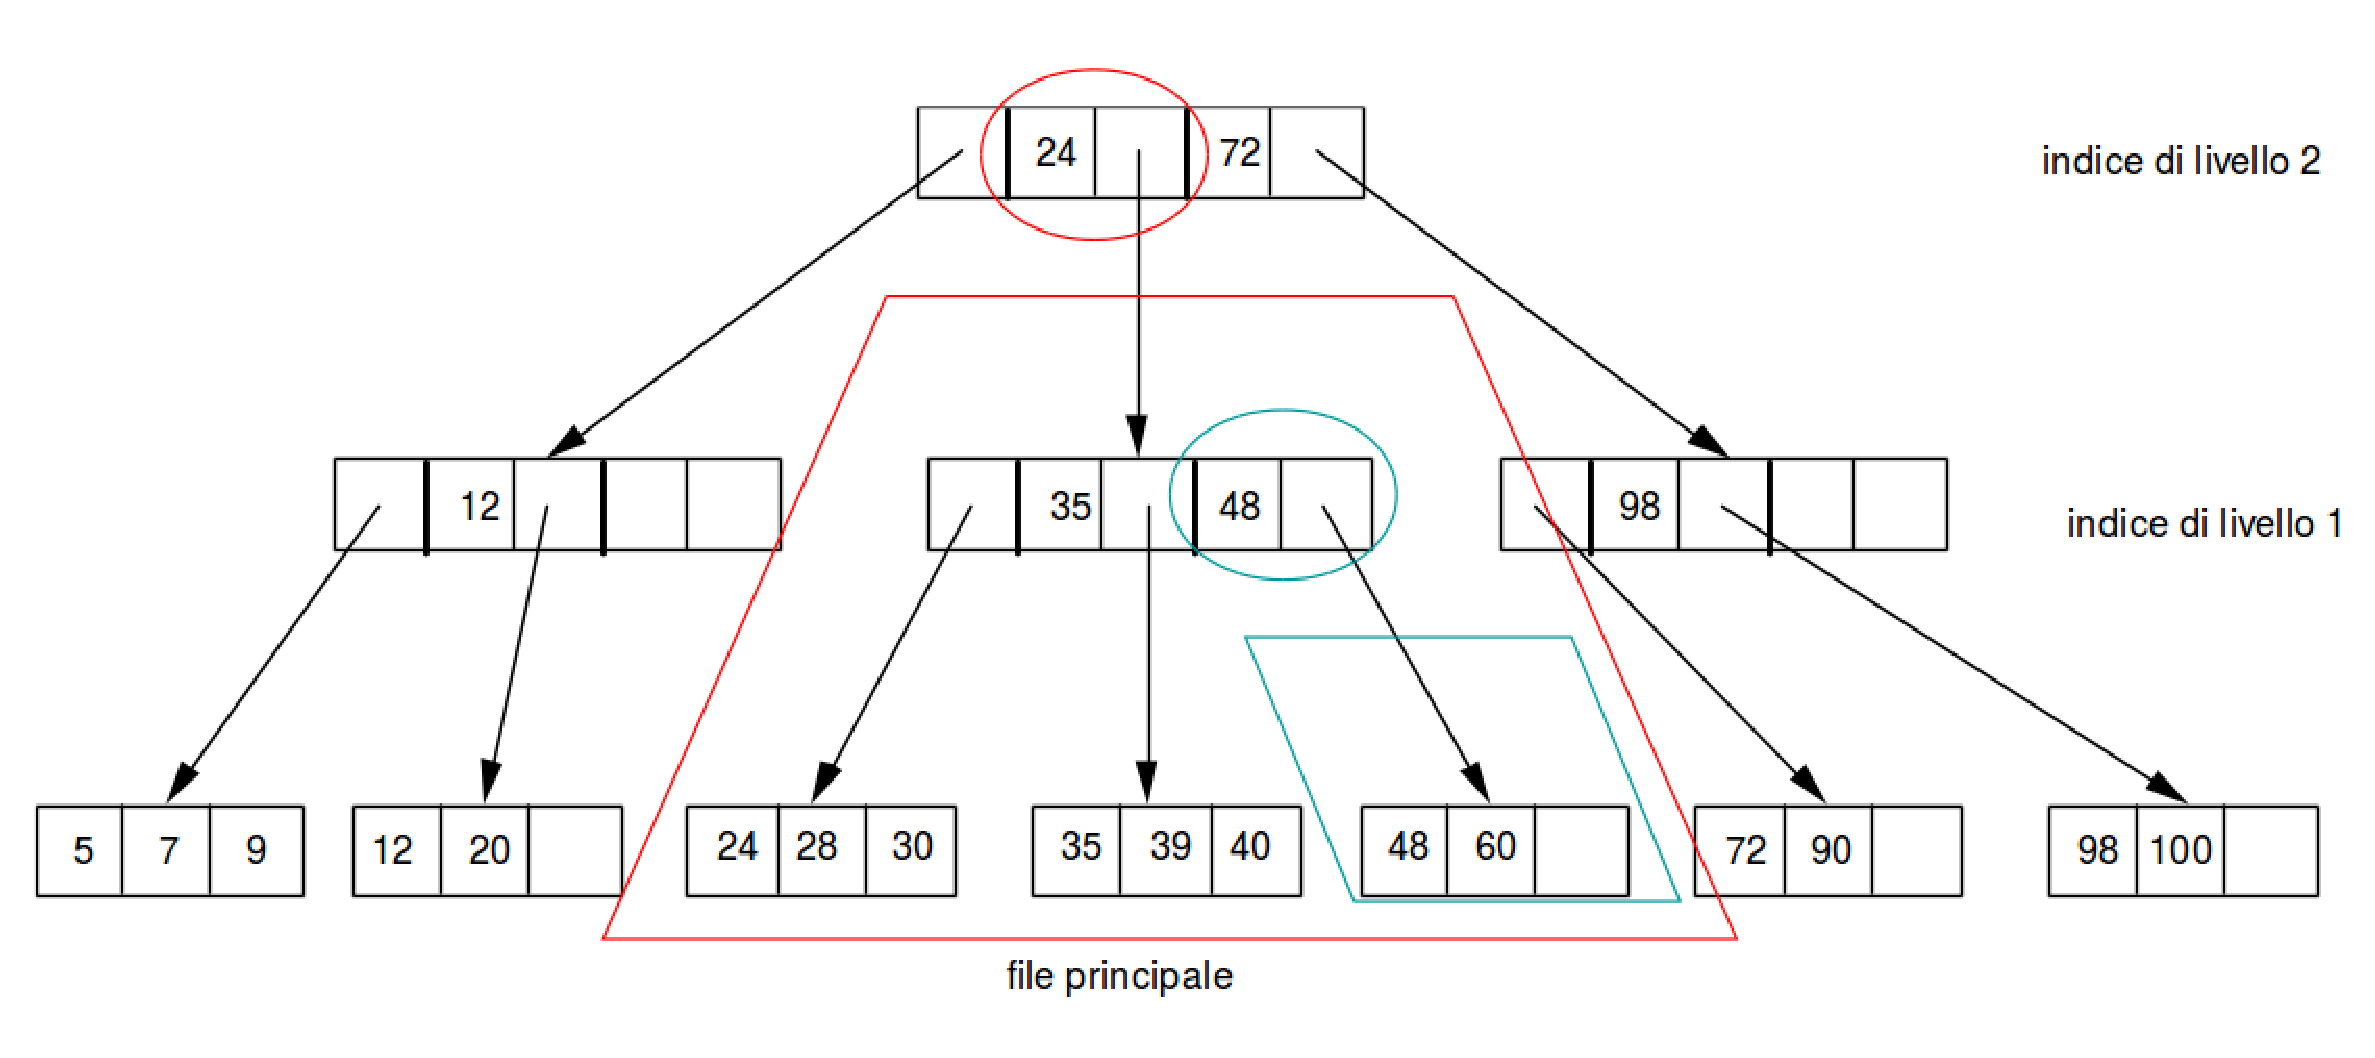
\includegraphics[width=430px]{img_5_3_4(1).eps}
  Figura 1
\end{figure}

e che si voglia inserire il record con valore della chiave $25$. Poiché il blocco (il terzo da sinistra) del
file principale in cui dovrebbe essere inserito tale record è pieno occorre richiedere al sistema un
nuovo blocco e ripartire i record del terzo blocco e il nuovo record fra il terzo blocco e il nuovo
blocco in modo da soddisfare il vincolo che ogni blocco deve essere pieno almeno per metà. Inoltre,
poiché il blocco del file indice di primo livello in cui dovrebbe essere inserito il puntatore al nuovo
blocco del file principale è pieno, occorre procedere per il file indice di livello $1$ allo stesso modo in
cui si è proceduto per il file principale, richiedendo un nuovo blocco al sistema. Ma allora un
analogo discorso deve essere fatto per l'indice di livello $2$. Pertanto dopo l'inserimento del record
con chiave $25$ il B-tree si presenterà come segue:

\begin{figure}[h!]
  \centering
  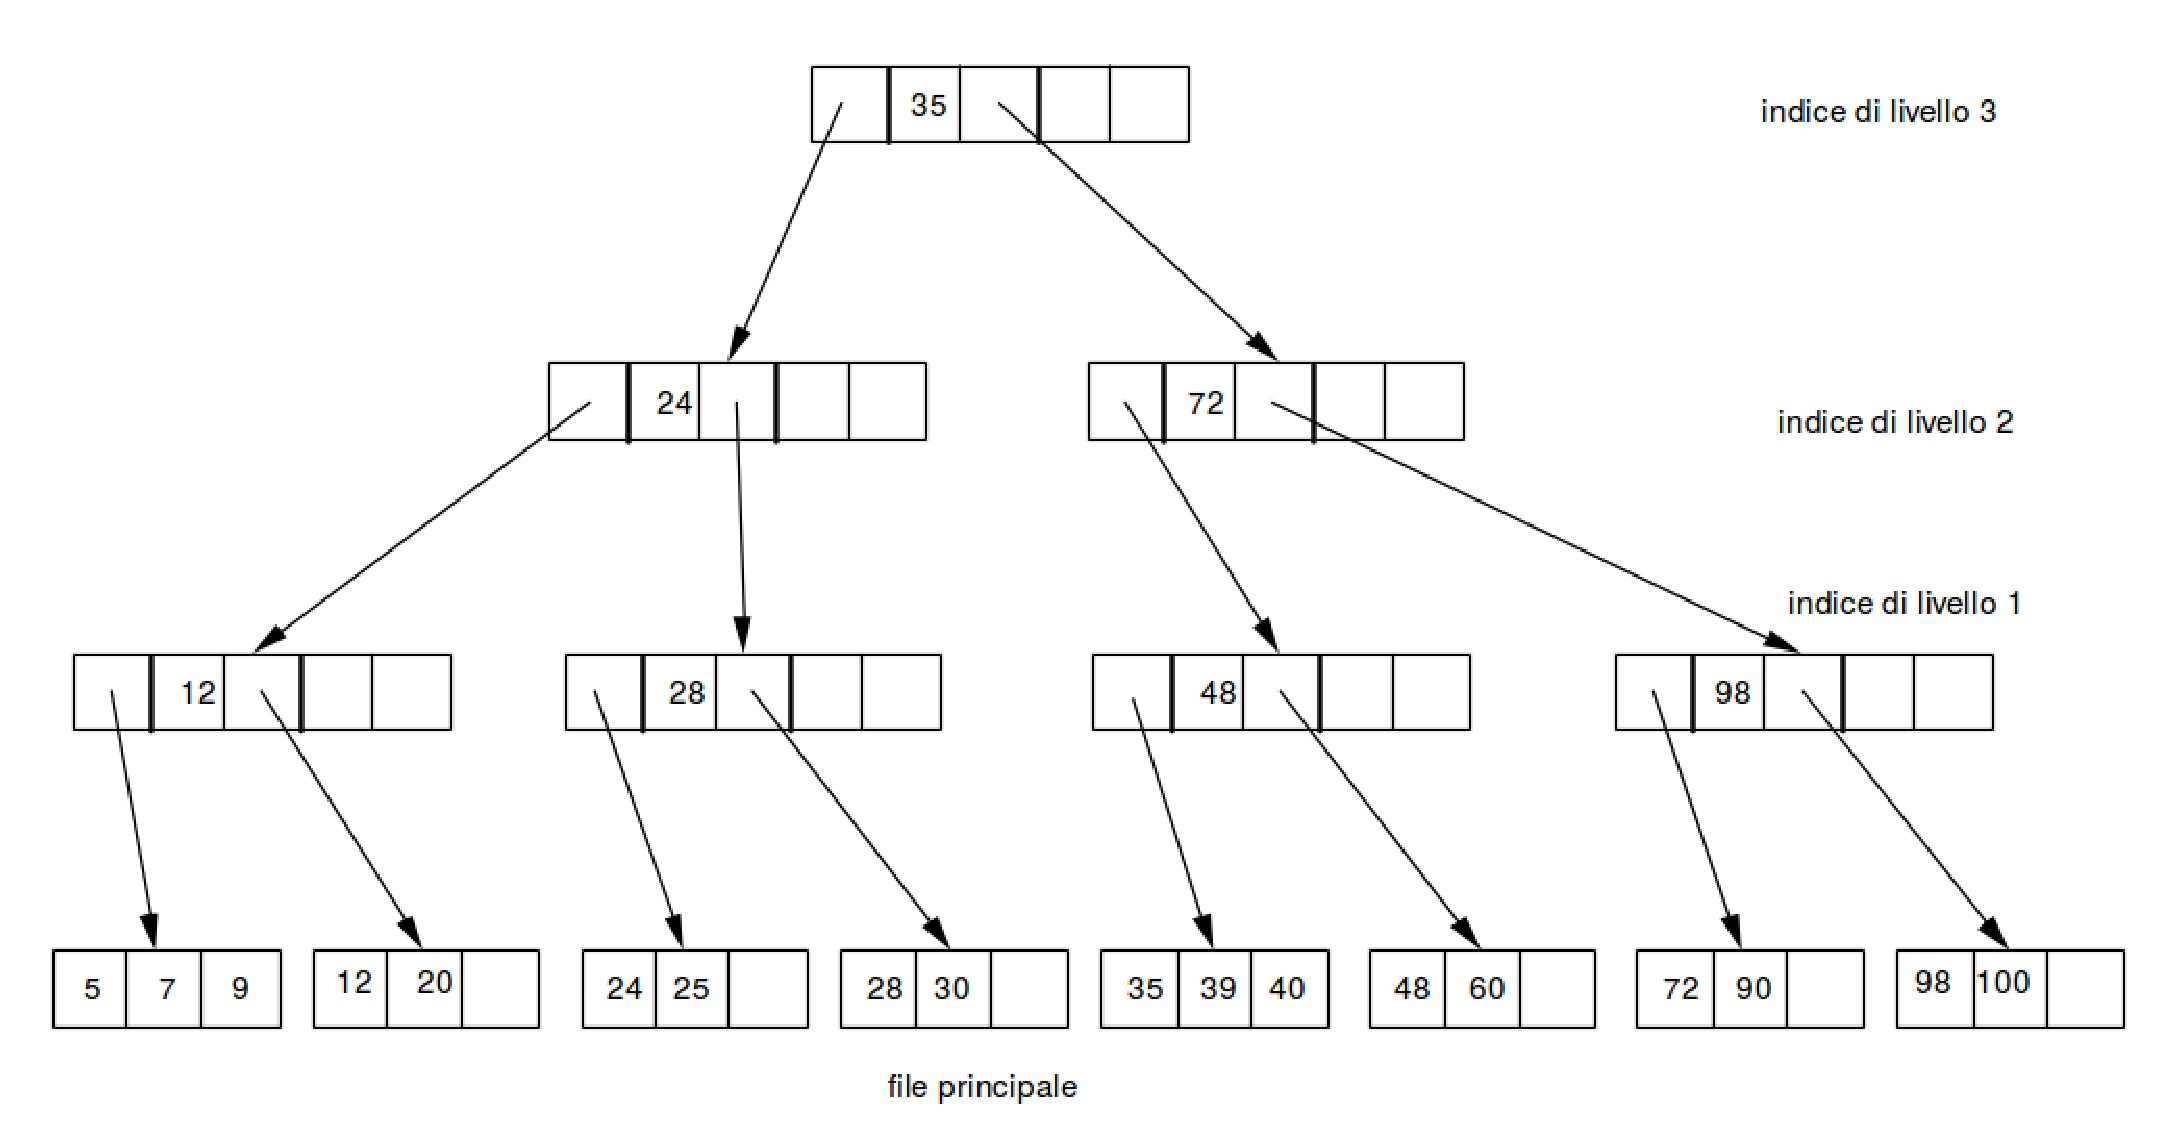
\includegraphics[width=430px]{img_5_3_4(2).eps}
  Figura 2
\end{figure}

Come si vede il numero dei livelli degli indici è aumentato di $1$, il che comporta un aumento dei
costi delle successive operazioni sul file principale.
Il numero di accessi necessari per effettuare la cancellazione del record con valore $v$ della chiave è
dato dal numero di accessi necessari per ricercare il blocco in cui si trova il record con chiave v più
uno per riscrivere il blocco, se il blocco rimane pieno almeno per metà successivamente alla
cancellazione. Se, viceversa, il blocco non rimane pieno almeno per metà successivamente alla
cancellazione, l'operazione può richiedere un numero ulteriore di accessi come mostra il seguente
esempio.\\
Supponiamo che in un certo istante la configurazione del B-tree sia quella mostrata in \textsc{Figura 2} e che si
voglia cancellare il record con chiave $28$. Poiché, a seguito della cancellazione di tale record nel
blocco rimane un solo record (e quindi non è soddisfatto il vincolo che ogni record debba essere
pieno al meno per metà), e tale record può trovare posto nel blocco precedente (il terzo da sinistra),
il blocco può essere restituito al sistema. Inoltre, poiché nel secondo blocco dell'indice di livello 1
rimane un solo puntatore possiamo procedere per l'indice di livello $1$ analogamente a come si è
proceduto per il file principale. Ma allora un analogo discorso deve essere fatto per l'indice di
livello $2$. Pertanto dopo la cancellazione del record con chiave $28$ il B-tree si presenterà come segue:

\begin{figure}[h!]
  \centering
  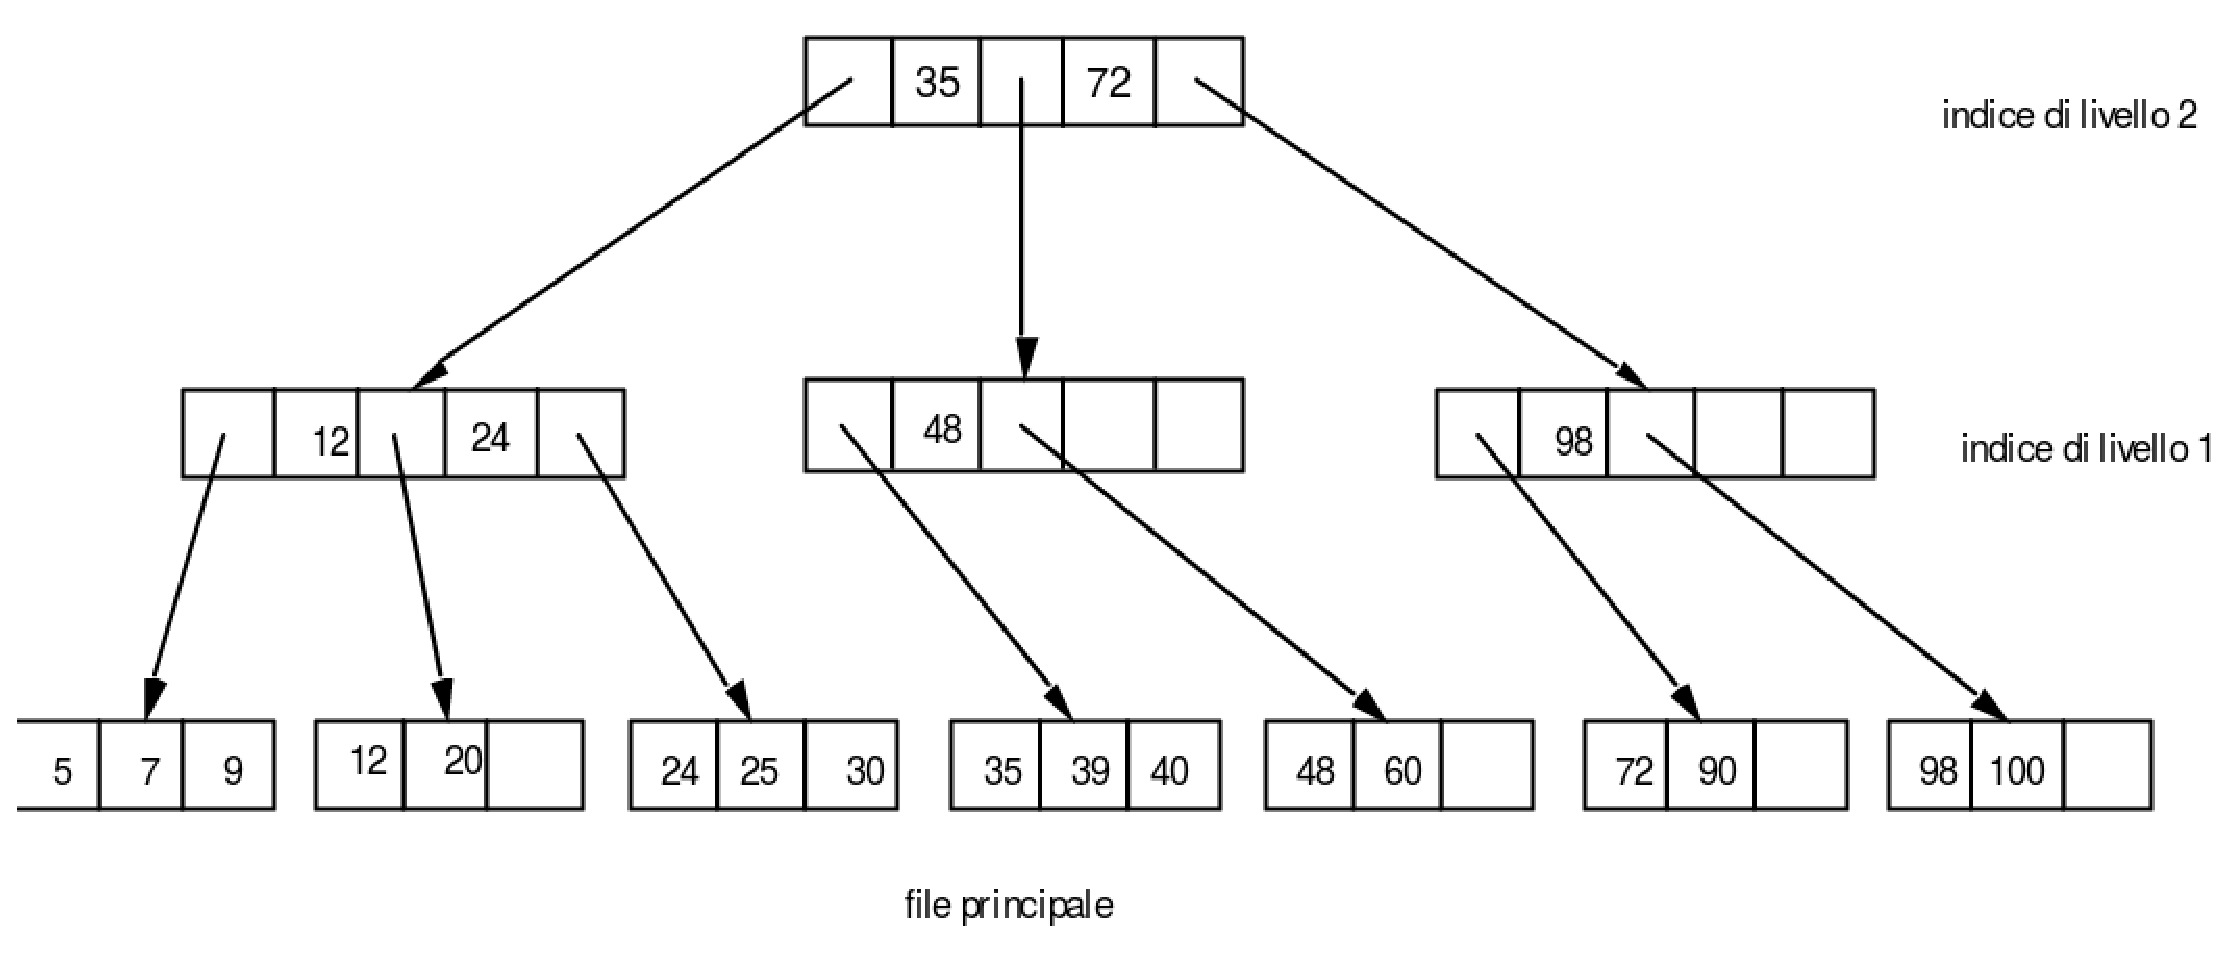
\includegraphics[width=400px]{img_5_3_4(3).eps}
  Figura 3
\end{figure}

Come si vede il numero dei livelli degli indici è diminuito di $1$, il che comporta una diminuzione dei
costi delle successive operazioni sul file principale.
Il numero di accessi necessari per effettuare la modifica del record con valore $v$ della chiave è dato
dal numero di accessi necessari per ricercare il blocco in cui si trova il record con chiave $v$ più uno
per riscrivere il blocco, se la modifica non coinvolge campi della chiave, altrimenti è dato dalla
somma degli accessi necessari per la cancellazione del record con chiave $v$ e quelli necessari per
l'inserimento del record con il nuovo valore della chiave.

\subsubsection{File con indice denso}
Nelle organizzazioni viste nei paragrafi precedenti, escluso l'heap, la maggior parte dei blocchi del
file principale non sono riempiti completamente; ciò comporta spreco di memoria e aumento dei
tempi di ricerca. D'altra parte, in un heap i blocchi sono completamente pieni, ma non si ha un
metodo efficiente per la ricerca di un record con un dato valore per la chiave.
Un tipo di organizzazione che cerca di cogliere gli aspetti positivi dell'uno e degli altri tipi di
organizzazione è il \textbf{file con indice denso}. Mentre nel caso di un file con indice sparso visto
precedentemente, ogni record del file indice contiene un puntatore per ogni blocco del file
principale, che è ordinato in base al valore della chiave, nel caso di un file con indice denso ogni
record del file indice contiene un puntatore ad un record del file principale, che non ha nessun tipo
di ordinamento.\\
Un indice denso è un file che può avere una qualsiasi delle organizzazioni viste precedentemente.
Per ricercare, cancellare o modificare un record del file principale, dato un valore per la chiave,
occorre ricercare il record con quel valore per la chiave nell'indice denso, fare un accesso per
leggere il blocco del file principale che contiene il record desiderato e, nel caso di modifica o
cancellazione, un accesso per riscrivere tale blocco. Nel caso di una cancellazione, occorre anche
cancellare nell'indice denso il record che ha il valore dato per la chiave. Per inserire un record si
procede nel modo seguente: si inserisce il record alla fine del file principale e quindi si inserisce
nell'indice denso il corrispondente record.\\
Apparentemente questo tipo di organizzazione sembra richiedere per ogni operazione qualche
accesso in più rispetto a quello che richiederebbe la stessa operazione se il file principale avesse la
stessa organizzazione scelta per l'indice denso. In realtà occorre tener presente che i costi di una
operazione di ricerca (e quindi di ogni operazione) dipendono dalle dimensioni del file (numero di
blocchi necessari per memorizzarlo) e che generalmente la dimensione dei record del file indice è
nettamente più piccola di quella dei record del file principale. Pertanto ogni operazione sul file
indice ha un costo inferiore di quello che avrebbe la stessa operazione se il file principale avesse la
stessa organizzazione scelta per l'indice denso.\\
L'uso di un indice denso permette anche di eliminare i puntatori a record del file principale: basta
sostituire ogni puntatore ad un record del file principale con il puntatore al corrispondente record
dell'indice denso. In tal modo per accedere al record occorre un accesso in più; d'altra parte se si
vuole muovere un record nel file principale è sufficiente modificare il puntatore nel corrispondente
record del file indice e, quindi, è possibile compattare il file principale riutilizzando lo spazio di
record cancellati. Un'altra alternativa è quella di sostituire ad ogni puntatore (che non si trovi
nell'indice denso) al file principale il valore della chiave e in base ad esso ricercare il record
utilizzando l'indice denso. Questa tecnica permette di compattare sia il file principale che il file
indice; tuttavia, mentre l'uso di un puntatore ad un record del file principale permette di raggiungere
il record con un unico accesso e quello di un puntatore al file indice permette di raggiungere il
record con due accessi, l' uso del valore della chiave come puntatore può richiedere un numero
superiore di accessi (quelli necessari per la ricerca sul file indice più un accesso al file principale)
per raggiungere il record.

\subsubsection{Strutture con record nidificati}
I metodi di organizzazione fisica visti nei paragrafi precedenti consentono la ricerca efficiente di un
record dato il valore della chiave. Spesso, però, è necessario effettuare su una base di dati un
diverso tipo di operazione consistente nel ricercare tutti i record che sono in qualche modo correlati
ad un dato record $r$ (ad esempio tutti i record $ORDINE$ relativi agli ordini fatti da un certo
$CLIENTE$). Perché questo tipo di ricerca possa essere effettuata in modo efficiente occorre che una
volta trovato il record $r$ sia possibile ritrovare i record ad esso correlati col minor numero di accessi
(ad esempio ogni record $ORDINE$ potrebbe trovarsi nello stesso blocco del record relativo al
$CLIENTE$ che lo ha fatto). In tal caso è implicita un a relazione gerarchica tra il record $r$ e i record
ad esso correlati. Per dare una rappresentazione lineare di tutte le possibili relazioni gerarchiche tra
record introduciamo il seguente concetto di pattern:
\begin{itemize}
 \item se $R$ è un tipo record, $R$ è un pattern le cui istanze sono tutte le occorrenze di un singolo record di
tipo $R$;
 \item se $P_1$, $P_2$, $\ldots, P_n$ sono pattern allora $P_1$, $P_2$, $\ldots, P_n$ è un pattern le cui istanze
 sono tutte le possibili sequenze $i_1, i_2, \ldots, i_n$ tali che $i_j$ è un'istanza di $P_j$;
 \item se $P$ è un pattern allora $(P)^*$ è un pattern le cui istanze sono sequenze (eventualmente vuote) di
istanze di $P$; un'istanza di $(P)^*$ è detta reapeating group.
\end{itemize}

Il modo più comune di memorizzare strutture gerarchiche è quello di memorizzare sequenzialmente
i record di ogni singola istanza di un pattern, ad esempio memorizzare sequenzialmente un record
relativo ad un cliente e i record di tutti gli ordini fatti da quel cliente. Un altro modo è quello di
rimpiazzare un repeating group con un puntatore ad un blocco che lo contiene; a tale puntatore può
essere associato il numero di istanze nel repeating group, altrimenti queste devono essere collegate
in una lista la cui fine è indicata da una marca di fine lista.\\
La necessità di rappresentare strutture gerarchiche è particolarmente forte nei sistemi gerarchici e
nei sistemi a rete, dove vengono utilizzati anche altri metodi di organizzazione (ad esempio un
repeating group può essere sostituito da un array di puntatori ai record del repeating group) oltre i
due sopra menzionati. Tuttavia ci sono dei sistemi relazionali che consentono di far uso di strutture
nidificate e, quindi, permettono di memorizzare in uno stesso blocco record appartenenti a relazioni
diverse.
Se un tipo record è coinvolto in una struttura nidificata e quindi le occorrenze di quel tipo record
sono memorizzate in modo che record correlati sono ``vicini'', non è possibile pensare di imporre sui
record di quel tipo di essere memorizzati in accordo a qualche tipo di organizzazione visto
precedentemente, come i file hash o i file ordinati (con indice). Pertanto se vogliamo poter accedere
ad un record in base al valore della chiave dobbiamo creare un indice denso. Ad esempio se
vogliamo accedere ad un record $ORDINE$ in base al numero dell'ordine e ogni record $ORDINE$ è
memorizzato ``vicino'' al record $CLIENTE$ relativo al cliente che ha fatto l'ordine, possiamo creare
un file hash o un file con indice i cui record contengono il numero di un ordine (chiave) e un
puntatore al relativo record $ORDINE$.

\subsubsection{Indici secondari}
Gli indici che abbiamo esaminato precedentemente, sia quelli sparsi che quelli densi, consentono di
ricercare un record in base al valore della chiave e prendono il nome di indici primari. Se vogliamo
ricercare i record che hanno un dato valore in un campo non chiave dobbiamo ricorrere ad un indice
secondario. 
\begin{defn}
 Un \textbf{indice secondario} è una struttura nidificata con il seguente pattern:
 \begin{center}
VALORE(RIFERIMENTO)$^*$  
 \end{center}
\end{defn}
Un'istanza di tale pattern è costituita da un valore del campo non chiave e da una sequenza di
riferimenti ai record che contengono quel valore in quel campo. Un riferimento può essere costituito
o da un puntatore al record o dal valore della chiave per quel record (i vantaggi e svantaggi di
ciascuna di tali scelte sono stati discussi precedentemente). In particolare, una struttura nidificata
con il pattern suddetto potrebbe essere usata per costruire un indice denso quando si è interessati ad
ricercare record del file principale in base al valore di un campo non chiave.
\newpage
\section{Concorrenza}

Un criterio per classificare i sistemi di gestione di basi di dati è il numero di utenti che possono
usare il sistema concorrentemente. Un sistema è \textbf{singolo-utente} se può essere usato da al più un
utente alla volta ed è \textbf{multiutente} se molti utenti possono usarlo contemporaneamente; la maggior
parte dei sistemi di gestione di basi di dati è del secondo tipo.\\
Se il sistema di calcolo ha più CPU allora è possibile il simultaneo processamento di due
programmi da parte di due diverse CPU; tuttavia la maggior parte della teoria del controllo della
concorrenza nelle basi di dati è stata sviluppata per sistemi di calcolo con una sola CPU. In tali
sistemi i programmi sono eseguiti concorrentemente in modo \emph{interleaved}, ovvero interfogliato: la CPU
può eseguire un solo programma alla volta, tuttavia il sistema operativo permette di eseguire alcune
istruzioni di un programma, sospendere quel programma, eseguire istruzioni di un altro programma
e quindi ritornare ad eseguire istruzioni del primo. In tal modo l'esecuzione concorrente dei
programmi è interleaved; ciò consente di tenere la CPU occupata quando un programma deve
effettuare operazioni di I/O.\\
\subsection{Scheduling di transazioni}
In un sistema di gestione di basi di dati multiutente la principale risorsa a cui i vari programmi
accedono concorrentemente è la base di dati. L'esecuzione di una parte di un programma che
rappresenta un'unità logica di accesso o modifica del contenuto della base di dati è detta
transazione. Ci sono sistemi (ad esempio le basi di dati statistici) in cui gli utenti effettuano solo
interrogazioni ma non modifiche; in tali sistemi l'esecuzione concorrente di più transazioni non crea
problemi. Al contrario nei sistemi in cui vengono effettuate da più utenti sia operazioni di lettura
che di scrittura (un tipico esempio di sistemi di questo tipo è costituito dai sistemi per la
prenotazione di posti sui voli) l'esecuzione concorrente di più transazioni può provocare problemi
se non viene controllata in qualche modo.\\
Prima di esaminare alcuni dei problemi che possono sorgere quando l'esecuzione concorrente di più
transazioni non è controllata, introduciamo il concetto di \textbf{schedule} (piano di esecuzione) di un
insieme di transazioni.
\begin{defn}
Dato un insieme $T$ di transazioni, uno \textbf{schedule} $S$ di $T$ è un ordinamento delle
operazioni nelle transazioni in $T$ tale che per ogni transazione $t$ in $T$ se $o_1$ e $o_2$ sono due operazioni
in $t$ tali che $o_1$ precede $o_2$ in $t$ allora $o_1$ precede $o_2$ in $S$.
\end{defn}
In altre parole uno schedule deve \emph{conservare l'ordine} che le operazioni hanno all'interno delle singole 
transazioni. Qualsiasi schedule ottenuto permutando le transazioni in $T$ è detto \emph{seriale}.
Consideriamo le seguenti transazioni

\begin{multicols}{2}  
 \begin{tabular}{|l|}
   \hline
   $t_1$\\
   \hline
   read(X)\\ 
   $X\vcentcolon=X-N$\\ 
   write(X)\\ 
   read(Y)\\
   $Y\vcentcolon=Y+N$\\
   write(Y)\\
   \hline
  \end{tabular} 
  
 \begin{tabular}{|l|}
  \hline
   $t_2$\\
   \hline
   read(X)\\ 
   $X\vcentcolon=X+M$\\ 
   write(X)\\
   \\
   \\
   \hline
  \end{tabular}\\
 \end{multicols}
 
 e i seguenti schedule di $\{t_1,t_2\}$:

 \begin{multicols}{2}  
 \begin{tabular}{|l|l|}
 \hline
 $t_1$ & $t_2$\\
 \hline
   read(X) & \\ 
   $X\vcentcolon=X-N$ & \\ 
   & read(X)\\
   & $X\vcentcolon=X+M$\\ 
   write(X) &\\ 
   read(Y) &\\
   & write(X)\\
   $Y\vcentcolon=Y+N$ &\\
   write(Y)&\\
   \hline
  \end{tabular}
  
  \begin{tabular}{|l|l|}
   \hline
   $t_1$ & $t_2$\\
   \hline
   read(X) & \\ 
   $X\vcentcolon=X-N$ & \\ 
   write(X) &\\ 
   & read(X)\\
   & $X\vcentcolon=X+M$\\ 
   & write(X)\\
   read(Y) &\\
   $t_1$ fallisce &\\
 
   \hline
  \end{tabular}
  
  
 \end{multicols}

Nel primo caso l'aggiornamento di $X$ prodotto da $t_1$ viene perso in quanto $t_2$ legge il valore di $X$
prima che l'aggiornamento prodotto da $t_1$ sia stato reso permanente. Nel secondo caso $t_2$ legge e
aggiorna il valore di $X$ dopo che l'aggiornamento prodotto da $t_1$ è stato reso permanente, ma prima
che venga ripristinato il vecchio valore di $X$ in conseguenza del fallimento di $t_1$.\\

Consideriamo ora una transazione $t_3$ che somma i valori di $X$ e di $Y$. Il seguente schedule di
$\{t_1, t_3\}$ fa sì che la somma prodotta da $t_3$ sia la somma del valore di $X$ dopo che $X$ è stato
aggiornato da $t_1$ e del valore di $Y$ prima che sia stato aggiornato da $t_1$.
\begin{center}
  \begin{tabular}{|l|l|}
   \hline
   $t_1$ & $t_3$\\
   \hline
   & $somma\vcentcolon=0$\\
   read(X) & \\ 
   $X\vcentcolon=X-N$ & \\ 
   write(X) &\\ 
   & read(X)\\
   & $somma\vcentcolon=somma + X$\\ 
   & read(Y)\\
   & $somma\vcentcolon= somma + Y$\\
   read(Y) &\\
   $Y\vcentcolon=Y+N$ &\\
   write(Y)&\\
   \hline
  \end{tabular}
\end{center}
In tutti e tre i casi visti siamo portati a considerare gli schedule non corretti in quanto i valori
prodotti non sono quelli che si avrebbero se le due transazioni fossero eseguite nel modo ``naturale''
cioè sequenzialmente.\\
In generale possiamo osservare che l'esecuzione naturale e, quindi, intuitivamente corretta di un
insieme di transazioni è quella \emph{sequenziale}; la possibilità di eseguire concorrentemente un insieme
di transazioni, come si è detto, è introdotta nei sistemi per motivi di efficienza. Pertanto tutti gli
schedule seriali sono corretti e uno schedule non seriale è corretto se è \emph{serializzabile}, cioè se è
``\textbf{equivalente}'' ad uno schedule seriale. Sorge quindi la necessità di definire un concetto di
equivalenza di schedule.\\
La più semplice definizione di equivalenza potrebbe essere basata sul confronto del risultato: due
schedule sono equivalenti se producono lo stesso stato finale. Tale definizione non è però
soddisfacente in quanto due schedule potrebbero produrre lo stesso stato finale solo per alcuni
valori iniziali. Consideriamo ad esempio le due transazioni 
\begin{multicols}{2}  
 \begin{tabular}{|l|}
   \hline
   $t_1$\\
   \hline
   read(X)\\ 
   $X\vcentcolon=X+5$\\ 
   write(X)\\ 
   \hline
  \end{tabular}

  \begin{tabular}{|l|}
  \hline
   $t_2$\\
   \hline
   read(X)\\ 
   $X\vcentcolon=X*1.5$\\ 
   write(X)\\
   \hline
  \end{tabular}

 \end{multicols}

 e i seguenti schedule di $\{t_1,t_2\}$:
\begin{multicols}{2}  
 \begin{tabular}{|l|l|}
 \hline
 $t_1$ & $t_2$\\
 \hline
   read(X) & \\
   & read(X)\\
   $X\vcentcolon=X+5$ & \\ 
   & $X\vcentcolon=X*1.5$\\
   & write(X)\\ 
   write(X) &\\ 
   \hline
  \end{tabular}

  \begin{tabular}{|l|l|}
   \hline
   $t_1$ & $t_2$\\
   \hline
   read(X) & \\
   & read(X)\\
   & $X\vcentcolon=X*1.5$\\
   $X\vcentcolon=X+5$ & \\ 
   write(X) &\\   
   & write(X)\\
   \hline
  \end{tabular}
 \end{multicols}
 
Tali schedule producono gli stessi valori solo se il valore iniziale di $X$ è $10$; ma producono valori
diversi in tutti gli altri casi. Problemi di questo tipo potrebbero essere evitati sfruttando proprietà
algebriche che garantiscano che il risultato sia lo stesso indipendentemente dai valori iniziali delle
variabili; tuttavia tale soluzione richiederebbe dei costi inaccettabili (che non sono giustificati dallo
scopo che si vuole raggiungere). Pertanto si fa l'assunzione più restrittiva che due valori sono
uguali solo se sono prodotti da esattamente la stessa sequenza di operazioni. Quindi, ad esempio,
date le due transazioni

\begin{multicols}{2}  
 \begin{tabular}{|l|}
   \hline
   $t_1$\\
   \hline
   read(X)\\ 
   $X\vcentcolon=X+N$\\ 
   write(X)\\ 
   \hline
  \end{tabular}



  \begin{tabular}{|l|}
  \hline
   $t_2$\\
   \hline
   read(X)\\ 
   $X\vcentcolon=X-M$\\ 
   write(X)\\
   \hline
  \end{tabular}

 \end{multicols}

 e i due schedule:
\begin{multicols}{2}  
 \begin{tabular}{|l|l|}
 \hline
 $t_1$ & $t_2$\\
 \hline
   read(X) & \\
   $X\vcentcolon=X+N$&\\ 
   write(X)&\\ 
   &read(X)\\ 
   &$X\vcentcolon=X-M$\\ 
   &write(X)\\
   \hline
  \end{tabular}

  \begin{tabular}{|l|l|}
   \hline
   $t_1$ & $t_2$\\
   \hline
   &read(X)\\ 
   &$X\vcentcolon=X-M$\\ 
   &write(X)\\
   read(X) & \\
   $X\vcentcolon=X+N$&\\ 
   write(X)&\\ 
   \hline
  \end{tabular}
 \end{multicols}
 
non sono considerati equivalenti.\\

Oltre alla definizione di equivalenza, un altro elemento che ha influenza sulla complessità del
problema di decidere se uno schedule è serializzabile (cioè se è equivalente ad uno schedule seriale)
è costituito dal fatto che il valore calcolato da una transazione per ogni dato sia \emph{dipendente} o meno
dal vecchio valore di quel dato. Nel primo caso il problema della serializzabilità può essere risolto
in tempo polinomiale con un semplice algoritmo su grafi; nel secondo caso il problema risulta
essere \emph{NP-completo}.\\
Nella pratica è difficile testare la serializzabilità di uno schedule. Infatti l'ordine di esecuzione delle
operazioni delle diverse transazioni è determinato in base a diversi fattori: il carico del sistema,
l'ordine temporale in cui le transazioni vengono sottomesse al sistema e le loro priorità. Pertanto è
praticamente impossibile determinare in anticipo come le operazioni saranno interleaved, cioè in
quale ordine verranno eseguite; d'altra parte, se prima si eseguono le operazioni e poi si testa la
serializzabilità dello schedule, i suoi effetti devono essere annullati se lo schedule risulta non
serializzabile. Inoltre quando le transazioni vengono sottomesse al sistema in modo continuo è
difficile stabilire quando uno schedule comincia e quando finisce. Quindi l'approccio seguito nei
sistemi è quello di determinare metodi che garantiscano la serializzabilità di uno schedule
eliminando così la necessità di dover testare ogni volta la serializzabilità di uno schedule. Uno di
tali metodi consiste nell'imporre dei protocolli, cioè delle regole, alle transazioni in modo da
garantire la serializzabilità di ogni schedule. Questi protocolli usano tecniche di \emph{locking} (cioè di
controllo dell'accesso ai dati) per prevenire l'accesso concorrente ai dati. Altri metodi di controllo
usano i \textbf{timestamp} delle transazioni, cioè degli identificatori delle transazioni che vengono generati
dal sistema e in base ai quali le operazioni delle transazioni possono essere ordinate in modo da
assicurare la serializzabilità.

\subsection{Item}
Tutte le tecniche per la gestione della concorrenza richiedono che la base di dati sia partizionata in
item, cioè in unità a cui l'accesso è controllato. Le dimensioni degli item devono essere definite in
base all'uso che viene fatto della base di dati in modo tale che in media una transazione acceda a
pochi item. Ad esempio se la transazione tipica su una base di dati relazionale è la ricerca di una
tupla mediante un indice, è appropriato trattare le tuple come item; se invece la transazione tipica
consiste nell'effettuazione di un join di due relazioni, è opportuno considerare le relazioni come
item. Le dimensioni degli item usate da un sistema sono dette la sua granularità. Una granularità
grande permette una gestione efficiente della concorrenza; una piccola granularità può invece
sovraccaricare il sistema, ma consente l'esecuzione concorrente di molte transazioni.

\subsection{Tecniche di locking per il controllo della concorrenza}
Queste tecniche fanno uso del concetto di lock. Un \textbf{lock} è un privilegio di accesso ad un singolo
item. In pratica è una variabile associata all'item il cui valore descrive lo stato dell'item rispetto alle
operazioni che possono essere effettuate su di esso. Un lock viene richiesto da una transazione
mediante un'operazione di locking e viene rilasciato mediante un'operazione di unlocking; fra
l'esecuzione di un'operazione di locking su un certo item $X$ e l'esecuzione di un'operazione di
unlocking su $X$ diciamo che la transazione mantiene un lock su $X$. Sono stati studiati diversi tipi di
lock; in ogni caso si assume che una transazione debba effettuare un'operazione di locking ogni
volta che deve leggere o scrivere un item e che l'operazione agisca come primitiva di
sincronizzazione, cioè se una transazione richiede un lock su un item su cui un'altra transazione
mantiene un lock, la transazione non può procedere finchè il lock non viene rilasciato dall'altra
transazione. Inoltre si assume che ciascuna transazione rilascia ogni lock che ha ottenuto. Uno
schedule è detto legale se obbedisce a queste regole.

\subsubsection{Lock binario}
Un \textbf{lock binario} può assumere solo due valori \emph{locked} e \emph{unlocked}. Le transazioni 
fanno uso di due operazioni \emph{lock(X)} e \emph{unlock(X)}; la prima serve per richiedere l'accesso
all'item $X$, la seconda per rilasciare l'item $X$ consentendone l'accesso ad altre transazioni. Se una 
transazione richiede l'accesso ad un item $X$ mediante un lock(X) e il valore della variabile è locked 
la transazione viene messa in attesa, altrimenti viene consentito alla transazione l'accesso ad $X$ e 
alla variabile associata ad $X$ viene assegnato il valore locked. 
Se una transazione rilascia un item $X$ mediante un unlock(X), alla variabile associata ad $X$ 
viene assegnato il valore unlocked; in tal modo se un'altra transazione è in attesa di accedere ad $X$ 
l'accesso gli viene consentito. Consideriamo di nuovo le due transazioni dell'esempio precedente e 
vediamo come l'uso dei lock può prevenire il problema dell'``aggiornamento perso''. 
Le transazioni $t_1$ e $t_2$ risultano modificate nel modo seguente 

\begin{multicols}{2}  

 \begin{tabular}{|l|}
   \hline
   $t_1$\\
   \hline
   lock(X)\\
   read(X)\\
   $X\vcentcolon=X-N$\\
   write(X)\\ 
   unlock(X)\\ 
   lock(Y)\\
   read(Y)\\
   $Y\vcentcolon=Y+N$\\
   write(Y)\\
   unlock(Y)\\
  \hline
 \end{tabular}
 
 \begin{tabular}{|l|}
  \hline
   $t_2$\\
   \hline
   lock(X)\\
   read(X)\\
   $X\vcentcolon=X+M$\\
   write(X)\\ 
   unlock(X)\\ 
  \\
  \\
  \\
  \hline
  \end{tabular}
  \\
 \end{multicols}

Uno schedule legale di $t_1$ e $t_2$ è il seguente:
\begin{center}
 \begin{tabular}{|l|l|}
 \hline
 $t_1$ & $t_2$\\
 \hline
   lock(X)&\\
   read(X)&\\
   $X\vcentcolon=X-N$&\\
   write(X)&\\ 
   unlock(X)&\\
   &lock(X)\\
   &read(X)\\
   &$X\vcentcolon=X+M$\\
   &write(X)\\ 
   &unlock(X)\\
   lock(Y)&\\
   read(Y)&\\
   $Y\vcentcolon=Y+N$&\\
   write(Y)&\\
   unlock(Y)&\\
   \hline
  \end{tabular}
\end{center}

Il più semplice modello per le transazioni è quello che considera una transazione come una
sequenza di operazioni di lock e unlock. Si assume che ogni operazione di lock su un item $X$ implica
la lettura di $X$ e ogni operazione di unlock di un item $X$ implica la scrittura di $X$. Il nuovo valore
dell'item viene calcolato da una funzione che è associata in modo univoco ad ogni coppia lock-unlock
ed ha per argomenti tutti gli item letti (locked) dalla transazione prima dell'operazione di
unlock. I valori che un item assume durante l'esecuzione di una transazione sono formule costruite
applicando le funzioni suddette ai valori iniziali degli item. Due schedule sono equivalenti se le
formule che danno i valori finali per ciascun item sono le stesse per i due schedule.\\
Consideriamo ad esempio le due transazioni seguenti:

\begin{multicols}{2}  

 \begin{tabular}{|l|}
   \hline
   $t_1$\\
   \hline
   lock(X)\\ 
   unlock(X)$f_1$(X)\\ 
   lock(Y)\\ 
   unlock(Y)$f_2$(X,Y)\\ 
  \hline
 \end{tabular}
 
 \begin{tabular}{|l|}
  \hline
   $t_2$\\
   \hline
   lock(Y)\\
   unlock(Y)$f_3$(Y)\\
   lock(X)\\
   unlock(X)$f_4$(X,Y)\\
  \hline
  \end{tabular} 
 \end{multicols}

e il seguente schedule $S$ di $t_1$ e $t_2$:
\begin{center}
 \begin{tabular}{|l|l|}
 \hline
 $t_1$ & $t_2$\\
 \hline
   lock(X)&\\
   unlock(X)&\\
   &lock(Y)\\
   &unlock(Y)\\
   lock(Y)&\\ 
   unlock(Y)&\\
   &lock(X)\\
   &unlock(X)\\
   \hline
  \end{tabular}
\end{center}
Se indichiamo con $X_0$ e $Y_0$ i valori iniziali di $X$ e $Y$, abbiamo che il valore finale per $X$ prodotto da $S$
è dato dalla formula $f_4(f_1(X_0), Y_0)$. D'altra parte il valore finale per $X$ prodotto dallo schedule
seriale $t_1$, $t_2$ è dato dalla formula $f_4(f_1(X_0), f_2(X_0, Y_0))$, mentre il valore finale per $X$ prodotto dallo
schedule seriale $t_2$, $t_1$ è dato dalla formula $f_1(f_4(X_0, Y_0))$; pertanto $S$ non è serializzabile in quanto
non è equivalente a nessuno schedule seriale di $\{t_1, t_2\}$.\\

\noindent Consideriamo ora le due transazioni seguenti
\begin{multicols}{2}  

 \begin{tabular}{|l|}
   \hline
   $t_1$\\
   \hline
   lock(X)\\ 
   unlock(X)$f_1$(X)\\ 
   lock(Y)\\ 
   unlock(Y)$f_2$(X,Y)\\ 
  \hline
 \end{tabular}
 
 \begin{tabular}{|l|}
  \hline
   $t_2$\\
   \hline
   lock(X)\\
   unlock(X)$f_3$(X)\\
   lock(Y)\\
   unlock(Y)$f_4$(X,Y)\\
  \hline
  \end{tabular} 
 \end{multicols}

e il seguente schedule $S$ di $t_1$ e $t_2$:
\begin{center}
 \begin{tabular}{|l|l|}
 \hline
 $t_1$ & $t_2$\\
 \hline
   lock(X)&\\
   unlock(X)&\\
   &lock(X)\\
   &unlock(X)\\
   lock(Y)&\\ 
   unlock(Y)&\\
   &lock(Y)\\
   &unlock(Y)\\
   \hline
  \end{tabular}
\end{center}

Se di nuovo indichiamo con $X_0$ e $Y_0$ i valori iniziali di $X$ e $Y$, abbiamo che il valore finale per $X$ e $Y$
prodotti da $S$ sono dati rispettivamente dalle formule $f_3(f_1(X_0))$ e $f_4(f_1(X_0), f_2(X_0, Y_0))$. Poiché tali
formule coincidono con quelle prodotte dallo schedule seriale \{$t_1, t_2\}$, lo schedule S è serializzabile.\\

La serializzabilità di uno schedule in questo semplice modello, può essere testata mediante un
semplice algoritmo su grafi diretti. L'idea su cui si basa tale algoritmo è la seguente. Dato uno
schedule, per ogni item si esamina l'ordine in cui le varie transazioni fanno un lock su quell'item; se
lo schedule è serializzabile questo ordine deve essere consistente con quello di uno schedule seriale;
pertanto se l'ordine imposto sulle transazioni da un certo item è diverso da quello imposto da un
altro item, lo schedule non è serializzabile. L'algoritmo lavora nel modo seguente.

\begin{alg}
Dato uno schedule S:
\begin{itemize}
 \item crea un grafo diretto $G$ (grafo di serializzazione) i cui nodi corrispondono alle transazioni; in
tale grafo c'è un arco diretto da $t_i$ a $t_j$ se in $S$ $t_i$ esegue un $unlock(X)$ e $t_j$ esegue il successivo
$lock(X)$ (il significato intuitivo dell'esistenza di un arco da $t_i$ a $t_j$ è che $t_j$ legge il valore per $X$
scritto da $t_i$ e quindi se esiste uno schedule seriale equivalente ad $S$ in tale shedule $t_i$ deve
precedere $t_j$);
\item verifica se $G$ ha un ciclo. Se $G$ ha un ciclo allora $S$ non è serializzabile; altrimenti esiste un
ordinamento $S'$ delle transazioni tale che $t_i$ precede $t_j$ se c'è in $G$ un arco diretto da $t_i$ a $t_j$; tale
ordinamento può essere ottenuto applicando a $G$ il procedimento noto come ordinamento
topologico consistente nell'eliminare ricorsivamente da un grafo diretto i nodi che non hanno
archi entranti (l'ordine di eliminazione dei nodi fornisce lo schedule seriale $S'$).
\end{itemize}
\end{alg}

Il seguente teorema prova la correttezza dell'algoritmo.
\label{teorema_6_1}
\begin{theo}
L'Algoritmo 1 determina correttamente se uno schedule è serializzabile. 
\end{theo}
\textbf{Dimostrazione.} Cominciamo con il dimostrare che se il grafo di serializzazione $G$ contiene un ciclo allora $S$
non è serializzabile. Supponiamo, per assurdo, che $G$ contenga un ciclo $t_1$, $t_2, \ldots, t_k$, $t_1$ e che
esista uno schedule seriale $S'$ equivalente ad $S$. Sia $t_i$, $1\leq i \leq k$, la transazione del ciclo che compare
per prima in $S'$ e sia $X$ l'item che causa la presenza in $G$ dell'arco da $t_i-1$ a $t_i$. Il valore finale per $X$
prodotto da $S'$ è dato da una formula in cui compare una funzione $f$ associata ad una coppia lockunlock
in $t_i-1$ e almeno uno degli argomenti di $f$ è una formula in cui compare una funzione $g$
associata ad una coppia lock-unlock in $t_i$. D'altra parte in $S$ l'effetto di $t_i-1$ su $X$ precede quello di $t_i$
su $X$ ; quindi nella formula che dà il valore finale per $X$ prodotto da $S$ la funzione f compare più
internamente di $g$ ($f$ è applicata prima di $g$). Pertanto $S'$ ed $S$ non sono equivalenti (contraddizione).
Mostriamo ora che se $G$ non ha cicli allora $S$ è serializzabile. A tal fine definiamo profondità di una
transazione $t$ la lunghezza del più lungo cammino in $G$ da un qualsiasi nodo a $t$.
Sia $S'$ lo schedule seriale costruito dall'algoritmo; mostreremo per induzione sulla profondità delle
transazioni che ogni transazione $t$ per ogni item su cui effettua un'operazione di lock legge in $S$ lo
stesso valore che legge in $S'$ (e quindi per ogni item su cui effettua un'operazione di lock produce in
$S$ lo stesso valore che produce in $S'$).
Base dell'induzione. Se per una transazione $t$ la profondità è 0 vuol dire che in $G$ non ci sono archi
entranti in $t$; pertanto in $S$ $t$ legge solo valori iniziali. D'altra parte in $S'$ $t$ viene prima di qualsiasi
transazione che effettua un'operazione di lock su un item su cui $t$ effettua un'operazione di lock.
Infatti, se $X$ è un item su cui $t$ effettua un'operazione di lock e $t_{i_1}, t_{i_2}, \ldots, t_{i_k}$ è la sequenza in $S$
delle transazioni che effettuano un'operazione di lock su $X$, $t_{i_1}, t_{i_2}, \ldots, t_{i_k}$ è un cammino in $G$;
poiché $t$ deve comparire in tale cammino e in $G$ non ci sono archi entranti in $t$, si deve avere $t=t_{i_1}$
e quindi nessun altro nodo del cammino può essere eliminato dal procedimento di ordinamento
topologico prima di $t$.
Induzione. Cominciamo con il mostrare che ogni transazione per ogni item su cui effettua
un'operazione di lock legge sia in $S$ che in $S'$ il valore prodotto da una stessa transazione.
Supponiamo, per assurdo, che esistano una transazione $t$ e un item $X$ tali che $t$ legge in $S$ il valore
di $X$ prodotto da una transazione $t'$ e in $S'$ il valore prodotto da un'altra transazione $t''$. Sia $t_{i_1},
t_{i_2}, \ldots, t_{i_k}$ la sequenza in $S$ delle transazioni che effettuano un'operazione di lock su $X$; $t_{i_1},
t_{i_2}, \ldots, t_{i_k}$ è un cammino in $G$ in cui $t'$ compare immediatamente prima di $t$. Anche $t''$ compare in tale
cammino, e quindi deve comparire prima di $t'$. Poiché in $S'$, $t''$ deve seguire $t'$, $S'$ non può essere
ottenuto da $G$ mediante il procedimento di ordinamento topologico (contraddizione).
Sia $t$ una transazione che ha profondità $d$, $d>0$, in $G$; per quanto visto $t$, per ogni item su cui
effettua un'operazione di lock, legge sia in $S$ che in $S'$ il valore prodotto da una stessa transazione
$t'$. Poiché $t'$ ha profondità minore di $d$ per l'ipotesi induttiva $t'$, per ogni item su cui effettua
un'operazione di lock, legge sia in $S$ che in $S'$ lo stesso valore e, quindi, produce sia in $S$ che in $S'$ lo
stesso valore. Pertanto $t$, per ogni item su cui effettua un'operazione di lock, legge sia in $S$ che in $S'$
lo stesso valore. \hfill $\Box$\\
\begin{defn}
Diciamo che una transazione obbedisce al protocollo di locking a due fasi, o più semplicemente che
è \textbf{a due fasi}, se prima effettua tutte le operazioni di lock (fase di locking) e poi tutte le operazioni di
unlock (fase di unlocking). 
\end{defn}
Mostreremo che il protocollo di locking a due fasi garantisce la serializzabilità; più precisamente, si ha che:
\begin{theo}
Sia $T$ un insieme di transazioni. Se ogni transazione in $T$ è a due fasi allora ogni
schedule di $T$ è serializzabile. 
\end{theo}
\textbf{Dimostrazione.} Sia $S$ uno schedule di $T$. Supponiamo, per assurdo, che $S$ non sia serializzabile. Per il
\linkto{teorema_6_1}{Teorema 6.1}, il grafo di serializzazione $G$ di $S$ contiene un ciclo $t_{i_1}, t_{i_2}, \ldots,
t_{i_k}$; ciò significa che $t_{i+1}$, $i\in \{1,\ldots k-1\}$, effettua un'operazione di lock, su un item su cui $t_i$
ha effettuato un'operazione di unlock e che $t_1$ effettua un'operazione di lock, su un item su cui $t_k$ ha effettuato
un'operazione di unlock. Pertanto in $S$ $t_1$ effettua un'operazione di lock dopo aver effettuato un'operazione di unlock
e quindi $t_1$ non è a due fasi (contraddizione).\\

Mostreremo ora che se una transazione $t_1$ non è a due fasi, esiste sempre una transazione $t_2$ tale
che esiste uno schedule di $\{t_1, t_2\}$ che non è serializzabile. Infatti, se $t_1$ non è a due fasi, effettua
un'operazione di lock dopo aver effettuato un'operazione di unlock; consideriamo anche la seguente transazione $t_2$  

\begin{multicols}{2}  

 \begin{tabular}{|l|}
   \hline
   $t_1$\\
   \hline
   $\ldots$\\
   unlock(X)\\ 
   $\ldots$\\
   lock(Y)\\ 
   $\ldots$\\
  \hline
 \end{tabular}
 
 \begin{tabular}{|l|}
  \hline
   $t_2$\\
   \hline
   lock(X)\\
   lock(Y)\\
   unlock(X)\\
   unlock(Y)\\
  \hline
  
  \end{tabular} 
 \end{multicols}

 il seguente schedule $S$ di $t_1$ e $t_2$ non è serializzabile
\begin{center}
 \begin{tabular}{|l|l|}
 \hline
 $t_1$ & $t_2$\\
 \hline
   $\ldots$&\\
   unlock(X)&\\
   $\ldots$&\\
   &lock(X)\\
   &lock(Y)\\
   &unlock(X)\\    
   unlock(Y)&\\
   $\ldots$&\\
   &lock(Y)\\
   $\ldots$&\\
   \hline
  \end{tabular}
\end{center}

Infatti il suo grafo di serializzazione
\begin{center}
  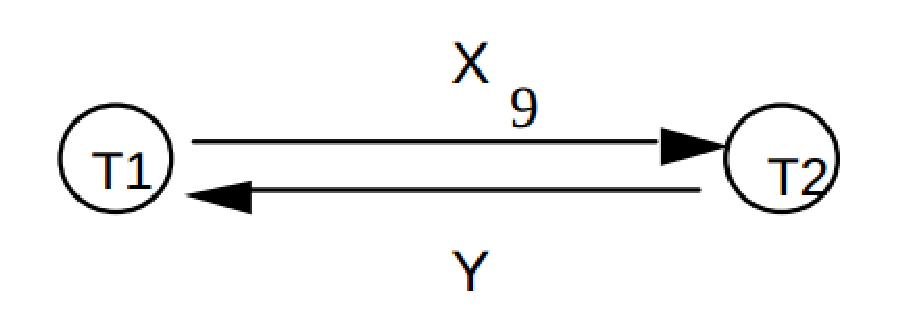
\includegraphics[width=150px]{img_6_3_1.eps}
\end{center}
contiene un ciclo. Naturalmente possono esistere schedule di transazioni che non sono a due fasi
che sono serializzabili. Tuttavia poiché è normale non conoscere l'insieme di transazioni con cui
una transazione può essere eseguita concorrentemente siamo costretti a richiedere che tutte le
transazioni siano a due fasi perché sia garantita la serializzabilità di ogni schedule.

\subsubsection{Lock a tre valori}
Consideriamo ora un modello per le transazioni che consente un maggior grado di concorrenza. In
tale modello si fa l'assunzione realistica che una transazione possa accedere ad un item solo per
leggerlo, senza modificarlo. Se una transazione desidera solo leggere un item $X$ effettua
un'operazione $rlock(X)$ che impedisce a qualsiasi altra transazione di modificare il valore di $X$;
tuttavia un qualsiasi numero di transazioni può ottenere contemporaneamente un lock di lettura su
$X$. Se, invece, una transazione desidera modificare il valore di $X$ effettua un'operazione $wlock(X)$; in
tal caso nessuna altra transazione può ottenere un lock di scrittura o di lettura su $X$. Entrambi i lock
sono rilasciati mediante un'operazione di $unlock(X)$. Pertanto si fa uso di un lock a tre valori:
$rlocked$, $wlocked$, $unlocked$.\\
Quanto detto per gli schedule legali vale anche in questo modello con l'unica differenza che una
transazione che mantiene un lock di lettura su un certo item può richiedere un lock in scrittura su
quello stesso item.\\
Analogamente a quanto fatto per il modello precedente assumiamo che quando una transazione
effettua un $wlock$ su un item il nuovo valore dell'item viene calcolato da una funzione,
univocamente associata a quell'operazione di $wlock$, che ha come argomenti tutti gli item su cui la
transazione ha già effettuato un lock (di lettura o di scrittura) prima dell'unlock associato al $wlock$.
Quindi, analogamente a quanto accadeva nel modello precedente, l'effetto di uno schedule sulla
base di dati può essere espresso dalle formule che calcolano (a partire dai valori iniziali degli item e
applicando le funzioni associate ai $wlock$) i valori degli item che sono modificati da almeno una
transazione. Tuttavia, poiché in questo modello si assume che una transazione possa leggere un item
senza modificarlo, la definizione di equivalenza di schedule deve essere modificata per tener conto
di tale eventualità.\\
\begin{defn}
 Due schedule sono \textbf{equivalenti} se:
 \begin{enumerate}
  \item producono lo stesso valore per ogni item su cui viene effettuato un wlock
  \item ogni operazione rlock(X) legge lo stesso valore di $X$ nei due schedule.
 \end{enumerate}
\end{defn}


Vediamo ora quali condizioni di precedenza tra transazioni è possibile inferire dalla semantica delle
transazioni appena vista.\\
Supponiamo che in uno schedule $S$ una transazione $t_1$ effettui un'operazione $wlock$ su un item $X$ e
che una transazione $t_2$ effettui un'operazione rlock su $X$ prima che una terza transazione $t_3$ esegua
la successiva operazione di $wlock$ su $X$ (in altre parole, $t_1$ modifica il valore di $X$ e $t_2$ legge il
valore di $X$ prodotto da $t_1$ prima che $X$ venga nuovamente modificato da $t_3$). Allora in qualsiasi
schedule seriale equivalente ad S $t_1$ deve precedere $t_2$ e $t_2$ deve precedere $t_3$. D'altra parte, se due
transazioni $t_1$ e $t_2$ leggono entrambe il valore di un item $X$ prodotto da una transazione non è lecito
stabilire nessuna precedenza tra $t_1$ e $t_2$ .
Per rappresentare le precedenze tra le transazioni è possibile usare, come per il modello precedente,
un grafo diretto che ha per nodi le transazioni e ha un arco da una transazione $t_i$ a una transazione
$t_j$ se la semantica delle transazioni impone che $t_i$ debba precedere $t_j$. Analogamente a quanto
accade per il modello precedente, un semplice algoritmo su tale grafo permette di decidere se uno
schedule è serializzabile e in caso affermativo di ottenere uno schedule seriale equivalente ad esso.

\begin{alg}
Dato uno schedule $S$
\begin{itemize}
 \item crea un grafo diretto $G$ (grafo di serializzazione) i cui nodi corrispondono alle transazioni; in
tale grafo c'è un arco diretto da $t_i$ a $t_j$ se
 \begin{itemize}
  \item in $S$ $t_i$ esegue una $rlock(X)$ o una $wlock(X)$ e $t_j$ è la transazione che esegue la successiva
   $wlock(X)$
  \item in $S$ $t_i$ esegue una $wlock(X)$ e $t_j$ esegue una $rlock(X)$ dopo che $t_i$ ha eseguito la $wlock(X)$ e
prima che un'altra transazione esegua una $wlock(X)$.
 \end{itemize}
\item verifica se $G$ ha un ciclo. Se $G$ ha un ciclo allora $S$ non è serializzabile; altrimenti esiste un
ordinamento $S'$ delle transazioni tale che $t_i$ precede $t_j$ se c'è in $G$ un arco diretto da $t_i$ a $t_j$; tale
ordinamento può essere ottenuto applicando a $G$ il procedimento di ordinamento topologico.
\end{itemize}
\end{alg}

Il seguente teorema, che può essere dimostrato con la stessa tecnica usata per il \linkto{teorema_6_1}{Teorema 6.1},
prova la correttezza dell'algoritmo.
\begin{theo}
L'Algoritmo 2 determina correttamente se uno schedule è serializzabile. 
\end{theo}

Consideriamo le seguenti transazioni:
\begin{multicols}{3}
 \begin{tabular}{|l|}
  \hline
  $t_1$\\
  \hline
  rlock(X)\\
  unlock(X)\\
  wlock(Y)\\
  unlock(Y)\\
  \hline
 \end{tabular}
 
  \begin{tabular}{|l|}
  \hline
  $t_2$\\
  \hline
  wlock(X)\\
  unlock(X)\\
  rlock(Z)\\
  unlock(Z)\\
  \hline
 \end{tabular}
 
  \begin{tabular}{|l|}
  \hline
  $t_1$\\
  \hline
  rlock(Y)\\
  unlock(Y)\\
  wlock(Z)\\
  unlock(Z)\\
  \hline
 \end{tabular}
\end{multicols}

Il seguente schedule di $\{t_1, t_2, t_3\}$ è serializzabile
\begin{center}
\begin{tabular}{|l|l|l|}
 \hline
 $t_1$ & $t_2$ & $t_3$\\
 \hline
 rlock(X)& &\\
 unlock(X)& &\\
 & wlock(X)& \\
 & unlock(X)& \\
 wlock(Y)& & \\
 unlock(Y)& &\\
 & & rlock(Y)\\
 & & unlock(Y)\\
 & &wlock(Z)\\
 & &unlock(Z)\\
 & rlock(Z)& \\
 & unlock(Z)& \\
\hline
 \end{tabular}
\end{center}

infatti il suo grafo di serializzazione
\begin{center}
 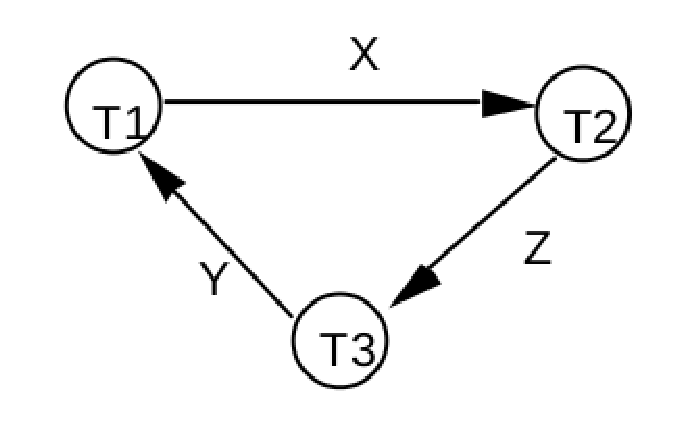
\includegraphics[width=150px]{img_6_3_2.eps}
\end{center}
contiene un ciclo.\\

Analogamente a quanto mostrato per il modello precedente anche per questo modello è possibile
dimostrare che qualsiasi schedule di un insieme di transazioni a due fasi (cioè transazioni in cui
nessuna operazione di lock può seguire una operazione di unlock) è serializzabile e che per qualsiasi
transazione $t$ a due fasi esiste uno schedule di transazioni contenente $t$ e almeno una transazione
non a due fasi che non è serializzabile.

\subsubsection{Read-only, write-only}
Nei due modelli di transazioni esaminati precedentemente viene fatta l'assunzione che ogni volta
che una transazione modifica un item $X$ legge il vecchio valore di $X$ e il nuovo valore di $X$ dipende
dal vecchio; in particolare nel primo modello l'insieme degli item letti e quello degli item scritti da
una transazione coincidono, mentre nel secondo modello l'insieme degli item scritti da una
transazione è contenuto nell'insieme degli item letti dalla stessa transazione. Un modello più
realistico dovrebbe prevedere che non ci sia necessariamente una relazione di contenimento tra
l'insieme degli item letti, \emph{read set}, e quello degli item scritti, \emph{write set}, da una transazione. Pertanto
considereremo ora un modello in cui, analogamente al modello precedente, una transazione può
effettuare operazioni di rlock e wlock, ma in cui:
\begin{enumerate}
 \item non si assume che quando una transazione scrive un item debba averlo letto
 \item non si assume che il valore di un item letto da una transazione sia significativo
indipendentemente dal fatto che abbia influenza sul valore finale di qualche item prodotto dalla
transazione.
\end{enumerate}
In conseguenza del punto 2, dovremmo considerare equivalenti due schedule se producono lo stesso valore
per ogni item su cui effettuano operazioni di scrittura. Una definizione di serializzabilità basata su
tale nozione di equivalenza non è però soddisfacente, come mostrato dall'esempio seguente.\\

Consideriamo lo schedule
\begin{center}
\begin{tabular}{|l|l|l|}
 \hline
 $t_1$ & $t_2$ & $t_3$\\
 \hline
 wlock(A)& &\\
 unlock(A)& &\\
 & wlock(C)& \\
 & unlock(C)& \\
 & rlock(A) & \\
 & rlock(B) &\\
  & unlock(A) &\\
  & unlock(B) &\\
 rlock(C) & &\\
 wlock(D) & &\\
 unlock(C)& & \\
 unlock(D)& & \\
 & & wlock(B)\\
 & & wlock(D)\\
 & & unlock(B)\\
 & & unlock(D)\\
\hline
 \end{tabular}
\end{center}


In base alla definizione di serializzabilità, detta \textbf{view serializability}, data sopra, tale schedule è
serializzabile; infatti i valori finali prodotti dallo schedule per gli item $A$, $B$, $C$ e $D$ sono i valori per
tali item calcolati rispettivamente dalle transazioni $t_1$, $t_3$, $t_2$ e $t_3$ e sono gli stessi valori prodotti
dallo schedule seriale $t_1$, $t_2$, $t_3$ . Tuttavia, se la transazione $t_3$ non viene eseguita (ad esempio per la
caduta del sistema) i valori finali prodotti per gli item $B$ e $D$ non coincidono né con i valori prodotti
dallo schedule seriale $t_1$, $t_2$, né con i valori prodotti dallo schedule seriale $t_2$, $t_1$.
Inoltre è stato dimostrato che se si adotta tale definizione di serializzabilità, il problema di decidere
se uno schedule è serializzabile risulta essere \emph{NP-completo}.\\
Prenderemo pertanto in esame un'altra definizione di serializzabilità, più restrittiva della
precedente, detta \textbf{conflict serializabilty}, basata su alcuni vincoli di precedenza imposti dalla
semantica delle transazioni; in base a tale definizione lo schedule appena visto risulta non
serializzabile.\\
Nel modello esaminato precedentemente se in uno schedule $S$ una transazione $t_1$ effettua un
$wlock(X)$ e $t_2$ è un'altra transazione che effettua il successivo $wlock(X)$ allora $t_2$ legge il valore di
$X$ scritto da $t_1$ e in base a tale valore calcola il nuovo valore di $X$; pertanto in qualsiasi schedule
seriale equivalente ad S $t_1$ deve precedere $t_2$ . Nel modello attualmente in esame, se $t_2$ non legge $X$
non c'è alcun motivo per cui debba seguire $t_1$ in uno schedule seriale equivalente ad $S$; in altre
parole due scritture successive di uno stesso item da parte di due distinte transazioni non
impongono nessun vincolo di precedenza. Vediamo quindi quali sono i vincoli che vanno
effettivamente imposti per uno schedule seriale equivalente ad uno schedule $S$:
\begin{enumerate}
 \item Se in $S$ una transazione $t_2$ legge il valore di un item $X$ scritto da una transazione $t_1$ allora $t_1$
deve precedere $t_2$ e,
 \item se $t_3$ è una terza transazione che scrive $X$ allora $t_3$ deve precedere $t_1$ o seguire $t_2$ .
\end{enumerate}
A tali vincoli devono essere aggiunti i seguenti:
\begin{enumerate}
\item se una transazione legge il valore iniziale di un item $X$ allora deve precedere qualsiasi
transazione che scriva $X$
\item se una transazione scrive il valore finale di un item $X$ allora deve seguire qualsiasi transazione
che scriva $X$.
\end{enumerate}

Se postuliamo l'esistenza all'inizio dello schedule di una transazione iniziale $t_0$ che scrive i valori
iniziali di tutti gli item (senza leggerne nessuno) e alla fine dello schedule di una transazione finale
$t_f$ che legge i valori finali di tutti gli item (senza scriverne alcuno), gli ultimi due vincoli sono
riassorbiti dal vincolo 1. Nel seguito dato uno schedule $S$ indichiamo con $S$ lo schedule ottenuto da
$S$ aggiungendo all'inizio la transazione iniziale e alla fine quella finale.\\

Diciamo allora che
\begin{defn}
 Uno schedule $S$ è serializzabile se esiste uno schedule seriale che rispetta tutti i
vincoli di tipo 1 e 2 generati da $S$.
\end{defn}

Analogamente a quanto visto per i modelli precedenti anche in questo caso possiamo rappresentare i
vincoli di precedenza imposti dalla semantica delle transazioni mediante gli archi in un particolare
tipo di grafo diretto. In particolare il vincolo 1 può essere rappresentato da un arco diretto $t_1\rightarrow t_2$ e
il vincolo 2 dalla coppia di archi alternativi $t_3\rightarrow t_1$ e $t_2\rightarrow t_3$. Una collezione di nodi, archi e
coppie di archi alternativi viene detta poligrafo. Un poligrafo è aciclico se almeno uno dei grafi che
possono essere ottenuti prendendo un arco da ogni coppia di grafi alternativi è aciclico.
Analogamente a quanto visto per i modelli precedenti, anche in questo caso la serializzabilità di uno
schedule può essere testata da un algoritmo che costruisce un poligrafo e quindi verifica se è
aciclico; inoltre, se è aciclico, fornisce (applicando l'ordinamento topologico ad un grafo aciclico
ottenuto dal poligrafo nel modo detto sopra) uno schedule seriale che rispetta i vincoli di
precedenza tra transazioni imposti dallo schedule dato. Prima di esaminare l'algoritmo osserviamo
che poiché in questo modello non si assume che il valore di un item letto da una transazione sia
significativo indipendentemente dal fatto che abbia influenza sul valore finale di qualche item
prodotto dalla transazione, una transazione che non ha alcun effetto sui valori finali prodotti da uno
schedule è considerata inutile in quello schedule. Come vedremo le transazioni inutili vengono
eliminate dall'algoritmo in quanto sono irrilevanti nel determinare la serializzabilità di uno schedule
(in altre parole una transazione inutile in uno schedule $S$ può leggere in $S$ e in uno schedule seriale
$S'$, che rispetta i vincoli di precedenza tra transazioni imposti da $S$, valori diversi).

\begin{defn}
Dato uno schedule $S$ i nodi del poligrafo $P$ sono le transazioni di $S$. 
\end{defn}

La costruzione degli archi di $P$ avviene attraverso i seguenti passi:
\begin{enumerate}
 \item vengono creati gli archi in accordo al vincolo 1; quindi se una transazione $t_2$ legge il valore di
un item $X$ scritto da una transazione $t_1$ viene aggiunto l'arco diretto $t_1\rightarrow t_2$
 \item vengono eliminati tutti gli archi entranti in transazioni inutili (una transazione inutile $t$ può
essere individuata facilmente perché non c'è nessun cammino in $P$ da $t$ a $t_f$)
 \item vengono creati gli archi in accordo al vincolo 2; quindi per ogni arco $t_1\rightarrow t_2$ se $t_3$ è transazione
distinta da quella iniziale che scrive un item che ha imposto l'esistenza dell'arco $t_1\rightarrow t_2$, si
aggiunge:
\begin{itemize}
 \item l'arco $t_2\rightarrow t_3$ se $t_1 = t_0$ e $t_2 \not= t_f$
 \item l'arco $t_3\rightarrow t_1$ se $t_2 = t_f$ e $t_1 \not= t_0$
 \item la coppia di archi alternativi $t_3\rightarrow t_1$ e $t_2\rightarrow t_3$ se $t_1 \not= t_0$ e $t_2 \not= t_f$.
\end{itemize}
\end{enumerate}

Si consideri il seguente schedule
\begin{center}
 \begin{longtable}{|l|l|l|l|}
  \hline
  $t_1$ & $t_2$ & $t_3$ & $t_4$\\
  \hline
  & rlock(A) & & \\
  rlock(A) & & & \\
  wlock(C) & & & \\
  unlock(C) & & & \\
  & & rlock(C) & \\
  wlock(B) & & & \\
  unlock(B)& & & \\
  & & & rlock(B)\\
  unlock(A) & & & \\
  & unlock(A)& &\\
  & & wlock(A)& \\
  & & & rlock(C)\\
  & wlock(D) & & \\
 & & & unlock(B)\\
  & &unlock(C)&\\
 & rlock(B) & & \\
  & & unlock(A)& \\
 & & & wlock(A)\\
 & unlock(B)& &\\
 & & & wlock(B)\\
 & & & unlock(B)\\
 & unlock(D) & &\\
   & & &unlock(C)\\
 & & & unlock(A)\\
\hline
 \end{longtable}
\end{center}
Le figure seguenti mostrano il poligrafo che viene costruito ai passi 1, 2 e 3 dell'algoritmo.
\begin{center}
\begin{figure}[h!]
\centering
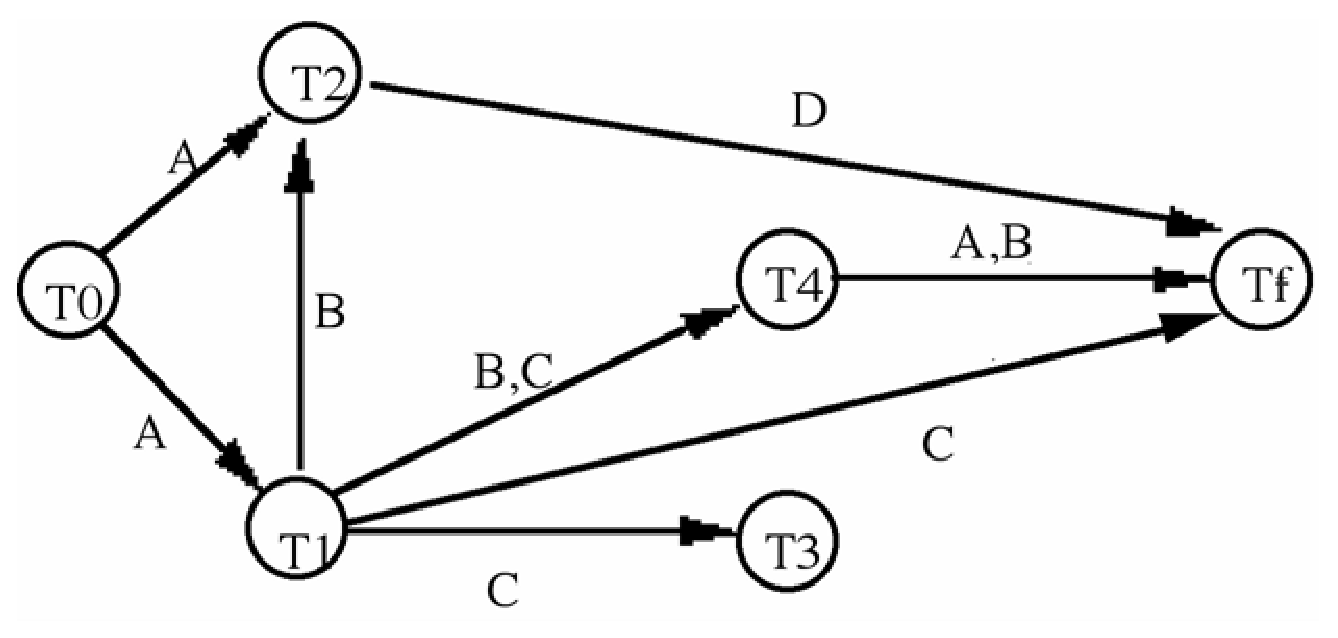
\includegraphics[width=200px]{img_6_3_2(1).eps}

Passo 1
\end{figure}

\begin{figure}[h!]
\centering
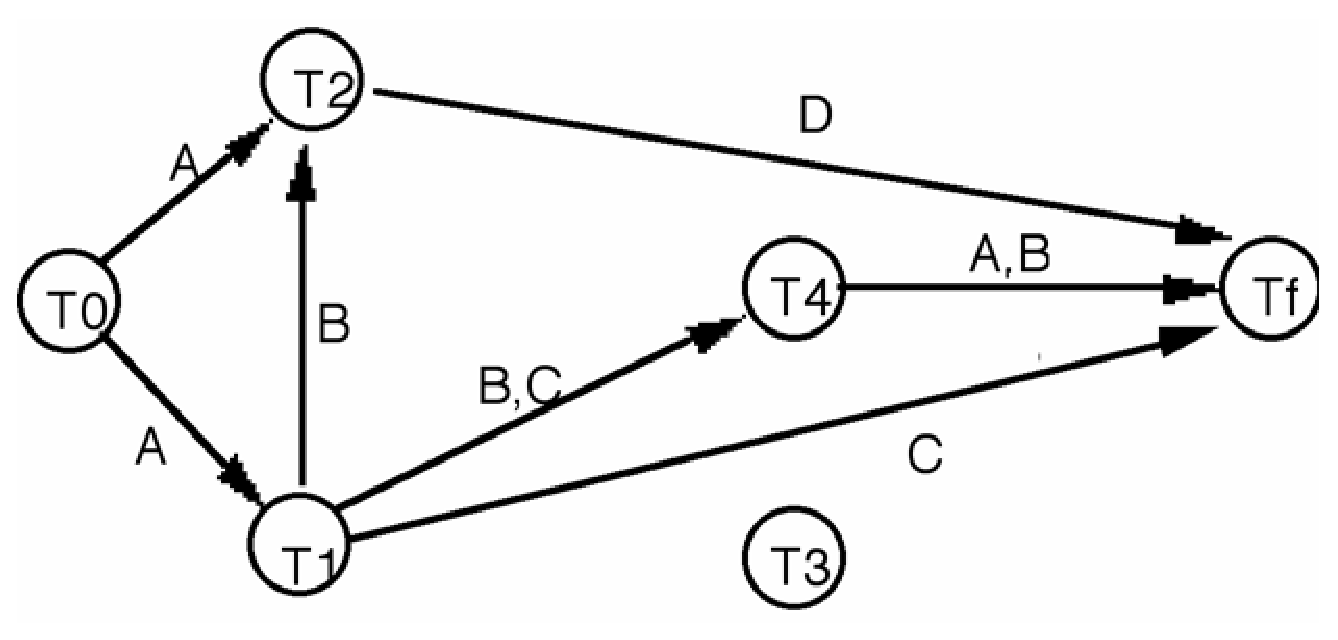
\includegraphics[width=200px]{img_6_3_2(2).eps}

Passo 2

\end{figure}

\begin{figure}[h!]
\centering
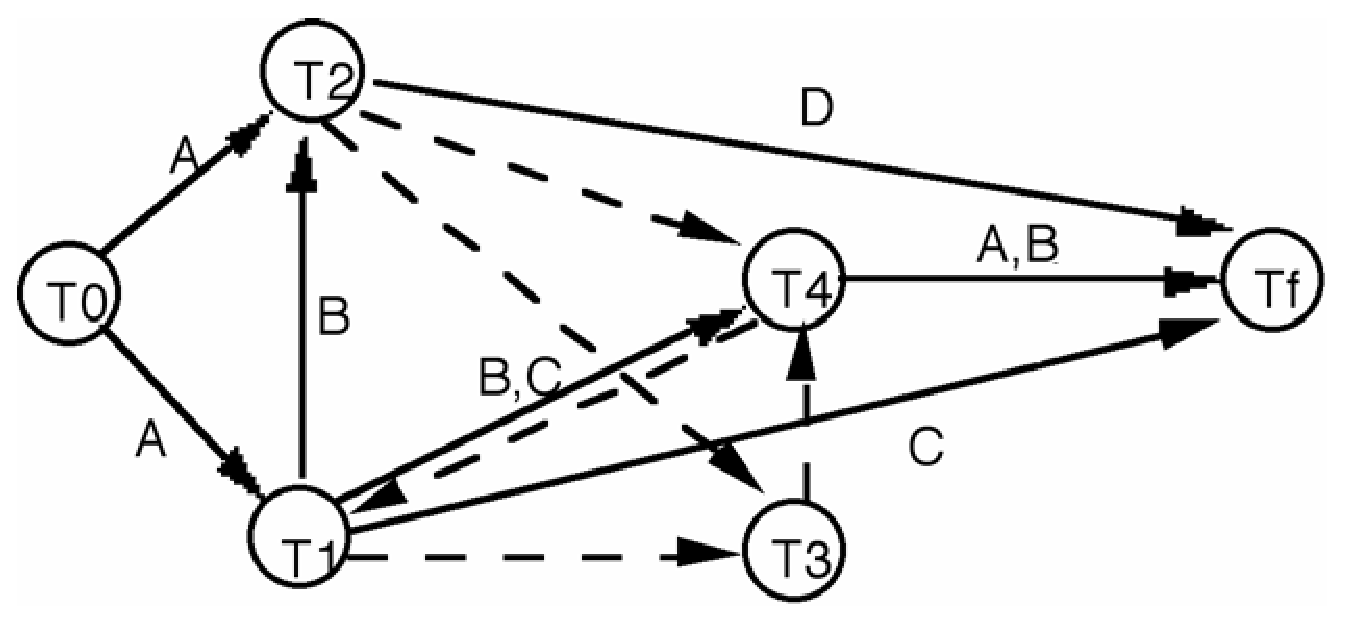
\includegraphics[width=200px]{img_6_3_2(3).eps}

Passo 3
\end{figure}
\end{center}

Poiché il poligrafo risultante è aciclico lo schedule è serializzabile e lo schedule seriale (che rispetta
i vincoli di precedenza tra transazioni imposti da esso) fornito dall'algoritmo è $t_1$, $t_2$, $t_3$,$t_4$.
Viceversa la figura seguente mostra il poligrafo costruito dall'algoritmo per lo schedule visto in
p recedenza; poiché contiene un ciclo, tale schedule non è serializzabile.
\begin{center}
 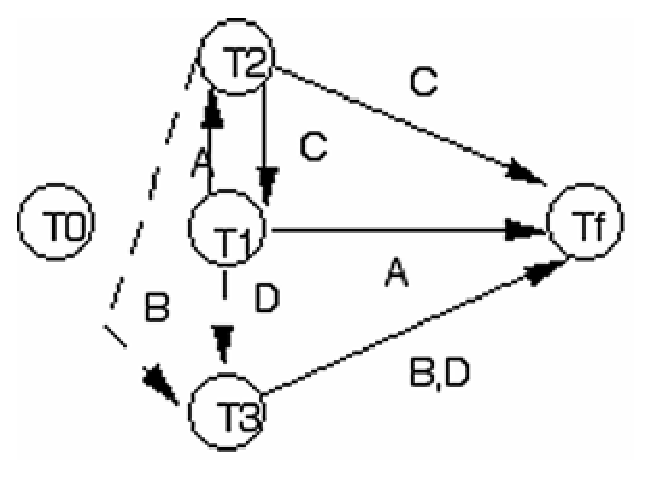
\includegraphics[width=150px]{img_6_3_2(4).eps}
\end{center}

\subsection{Deadlock e livelock}
In un sistema che utilizza i lock per il controllo della concorrenza si possono verificare delle
situazioni anomale note con il nome di \emph{deadlock} e \emph{livelock}.\\
Un \textbf{livelock} si verifica quando una transazione aspetta indefinitamente che gli venga garantito un
lock su un certo item. Ad esempio, consideriamo il caso di una transazione $t$ in attesa di effettuare
un lock su un item $X$ su cui un'altra transazione $t_1$ mantiene un lock; se quando $t_1$ rilascia $X$
un'altra transazione $t_2$ ottiene un lock su $X$, $t$ deve rimanere in attesa; poiché questa situazione può
ripeter si un numero indefinito di volte, $t$ può rimanere indefinitamente in attesa di ottenere un lock
su $X$.\\
Un \textbf{deadlock} si verifica quando ogni transazione in un insieme $T$ è in attesa di ottenere un lock su
un item sul quale qualche altra transazione in $t$ mantiene un lock.\\
Entrambi i problemi si possono presentare in un qualsiasi sistema in cui i processi possono essere
eseguiti concorrentemente e quindi sono stati largamente studiati nell'ambito dei sistemi operativi.
Il primo problema può essere risolto con una strategia first \emph{came-first served}; in altre parole il
sistema mantiene memoria delle successive richieste di lock in modo che, quando un item $X$ viene
rilasciato, viene garantito un lock su $X$ alla transazione che per prima ha richiesto un lock su $X$.
Un'altra possibile strategia può essere quella di eseguire le transazioni in base alle loro priorità e di
aumentare la priorità di una transazione all'aumentare del tempo in cui rimane in attesa in modo che
possa ad un certo punto assumere la priorità più alta ed essere eseguita.\\
Per risolvere il secondo problema possono essere seguiti due approcci. Un approccio è preventivo in
quanto cerca di evitare il verificarsi di situazioni di stallo adottando opportuni protocolli; l'altro
invece si preoccupa di risolvere le situazioni di stallo quando si verificano. Il sussistere di una
situazione di stallo può essere rilevato mantenendo un grafo di attesa, cioè un grafo i cui nodi sono
le transazioni e in cui c'è un arco $t_1$ →$t_2$ se la transazione $t_1$ è in attesa di ottenere un lock su un
item sul quale $t_2$ mantiene un lock; se in tale grafo c'è un ciclo si sta verificando una situazione di
stallo che coinvolge le transazioni nel ciclo; per risolverla occorre che almeno una transazione nel
ciclo sia \emph{rolled-back}. Una transazione è \textbf{rolled-back} quando viene abortita, 
i suoi effetti sulla base di dati vengono annullati ripristinando i valori dei dati precedenti 
l'inizio della sua esecuzione e, infine, tutti i lock mantenuti dalla transazione vengono rilasciati.
Una volta fatto ciò viene fatta ripartire.

\subsection{Protocollo di locking a due fasi stretto}
Oltre al verificarsi di un deadlock, ci sono altri motivi per cui una transazione deve essere abortita,
ad esempio perché ha cercato di effettuare un accesso non autorizzato oppure perché ha cercato di
eseguire una divisione per 0. Il punto in cui una transazione non può più essere abortita per uno dei
suddetti motivi, cioè il punto in cui ha ottenuto tutti i lock che gli sono necessari e ha effettuato tutti
i calcoli nell'area di lavoro, viene detto \textbf{punto di commit} della transazione; una transazione che ha
raggiunto il suo punto di commit viene detta \emph{committed} altrimenti viene detta \emph{attiva}. Quando una
transazione raggiunge il suo punto di commit effettua un'operazione di commit (nei sistemi reali
tale operazione prevede lo svolgimento di diverse azioni, ma per i nostri scopi serve solo a marcare
il punto di commit della transazione). I dati scritti da una transazione sulla base di dati prima che
abbia raggiunto il punto di commit vengono detti dati sporchi. Il fatto che un dato sporco possa
essere letto da qualche altra transazione può causare un effetto di roll-back a cascata.\\

Consideriamo il seguente schedule
\begin{center}
 \begin{longtable}{|l|l|}
 \hline
 $t_1$ & $t_2$\\
 \hline
wlock(X) & \\
read(X)& \\
$X\vcentcolon=X-N$& \\
write(X)& \\
unlock(X)& \\
 &rlock(X)\\
 &wlock(Z)\\
 &read(X)\\
 &read(Z)\\
 &$Z\vcentcolon=Z+X$\\
 &write(Z)\\
 &commit\\
 &unlock(X)\\
 &unlock(Z)\\
 wlock(Y)& \\
 read(Y)& \\
 $Y\vcentcolon=Y+N$& \\
 write(Y)& \\
 commit& \\
 unlock(Y)& \\
 \hline
 \end{longtable}
\end{center}

Se la transazione $t_1$ viene abortita dopo che ha letto $Y$, il valore di $X$ scritto da $t_1$ è un dato
sporco; infatti, quando $t_1$ viene abortita è necessario annullare gli effetti di $t_1$ sulla base di dati
ripristinando il vecchio valore di $X$ (quello letto da $t_1$). Ma allora è necessario annullare anche gli
effetti di $t_2$ sulla base di dati in quanto il valore di $Z$ prodotto da $t_2$ è calcolato a partire dal valore
di $X$ scritto $t_1$. Pertanto sia $t_1$ che $t_2$ devono essere rolled-back.\\
Per evitare questo fenomeno detto rollback a cascata occorre impedire alle transazioni di leggere
dati sporchi. Ciò può essere ottenuto adottando un protocollo di locking a due fasi stretto.
\begin{defn}
 Una transazione soddisfa il protocollo a due fasi stretto se:
 \begin{enumerate}
  \item non scrive sulla base di dati fino a quando non ha raggiunto il suo pun to di commit
  \item non rilascia un lock finchè non ha finito di scrivere sulla base di dati.
 \end{enumerate}
\end{defn}

La condizione 1 garantisce che se una transazione è abortita allora non ha modificato nessun item
nella base di dati; la condizione 2 garantisce che quando una transazione legge un item scritto da
un'altra transazione quest'ultima non può essere abortita (quindi nessuna transazione legge dati
sporchi).\\
Perché la transazione $t_1$ nell'esempio precedente soddisfi il protocollo di locking a due fasi stretto
deve essere modificata nel modo seguente.

\begin{center}
 \begin{tabular}{|l|}
  \hline
  $t_1$\\
  \hline
wlock(X)\\
read(X)\\
$X\vcentcolon=X-N$\\
wlock(Y)\\
read(Y)\\
$Y\vcentcolon=Y+N$\\
commit\\
write(X)\\
write(Y)\\
unlock(X)\\
unlock(Y)\\
\hline
 \end{tabular}
\end{center}

I protocolli di locking a due fasi stretti possono essere classificati in \emph{protocolli conservativi} e
\emph{protocolli aggressivi}; i primi cercano di evitare il verificarsi di situazioni di stallo, i secondi cercano
di processare le transazioni il più rapidamente possibile anche se ciò può portare a situazioni di
stallo e, quindi, alla necessità di abortire qualche transazione.\\

La versione più conservativa di un protocollo di locking a due fasi stretto è quella che impone ad
una transazione di richiedere all'inizio tutti gli item di cui può avere bisogno. Lo scheduler permette
alla transazione di procedere solo se tutti i lock che ha richiesto sono disponibili, altrimenti la mette
in una coda di attesa. In tal modo non possono verificarsi deadlock, ma possono ancora verificarsi
livelock. Per evitare anche il verificarsi di livelock si può impedire ad una transazione $t$ di
procedere (anche se tutti i lock da essa richiesti sono disponibili) se c'è un'altra transazione che
precede $t$ nella coda che è in attesa di ottene re un lock richiesto da $t$. \`E facile vedere che se si
adotta un protocollo in cui tutti i lock sono richiesti all'inizio e uno scheduler che garantisce ad una
transazione $t$ tutti i lock richiesti se e solo se:
\begin{enumerate}
 \item tutti i lock sono disponibili
 \item nessuna transazione che precede $t$ nella coda è in attesa di un lock richiesto da $t$
\end{enumerate}
allora non si possono verificare né dealdock né livelock. Infatti per la condizione 1 nessuna
transazione che mantiene un lock può essere in attesa di un lock mantenuto da un'altra transazione;
inoltre, la condizione 2 garantisce che dopo un tempo finito ogni transazione raggiunge la testa della
coda e quindi viene eseguita.\\
Il protocollo conservativo esaminato presenta due inconvenienti. Infatti l'esecuzione di una
transazione può essere ritardata dal fatto che non può ottenere un lock anche se molti passi della
transazione potrebbero essere eseguiti senza quel lock; inoltre una transazione è costretta a
richiedere un lock su ogni item che potrebbe essergli necessario anche se poi di fatto non l'utlizza.
Ad esempio, se una transazione deve effettuare una ricerca su un file con indice sparso e gli item
sono i blocchi, la transazione deve effettuare un lock su ogni blocco del file principale e del file
in dice anche se poi accederà soltanto ad alcuni blocchi del file indice e ad un solo blocco del file
principale.\\

La versione più aggressiva di un protocollo di locking a due fasi stretto è quella che impone ad una
transazione di richiedere un lock su un item immediatamente prima di leggerlo o scriverlo. Se le
transazioni soddisfano tale protocollo possono verificarsi situazioni di stallo; un modo per evitare
ciò è quello di definire un ordinamento sugli item e di imporre alle transazioni di richiedere i lock in
accordo a tale ordinamento. In tal modo non possono verificarsi deadlock. Infatti, sia $T$ un insieme
di transazioni (che richiedono i lock in accordo all'ordinamento fissato sull'insieme degli item) tale
che ogni transazione $t_k$ è in attesa di un item $A_k$ e mantiene un lock su almeno un item (si osservi
che se una transazione $t$ in $T$ non soddisfa la seconda condizione allora l'insieme $T-\{t\}$ è ancora
un insieme di transazioni in stallo) e sia $A$ i il primo item nell'ordinamento fissato sull'insieme degli
item; allora la transazione $t_i$ che è in attesa di $A_i$ non può mantenere un lock su alcun item
(contraddizione). Tuttavia il metodo di ordinare gli item non è molto praticabile perché non sempre
una transazione può scegliere l'ordine in cui richiedere i lock.\\
Un protocollo aggressivo è adatto a situazioni in cui la probabilità che due transazioni richiedano un
lock su uno stesso item è bassa (e quindi è bassa la probabilità che si verifichi una situazione di
stallo), in quanto evita al sistema il sovraccarico dovuto alla gestione dei lock (decidere se garantire
un lock su un dato item ad una data transazione, gestire la tavola dei lock, mettere le transazioni in
una coda o prelevarle da essa). Un protocollo conservativo è invece adatto a situazioni opposte in
quanto evita al sistema il sovraccarico dovuto alla gestione dei deadlock (rilevare e risolvere
situazioni di stallo, eseguire parzialmente transazioni che poi vengono abortite, rilascio dei lock
mantenuti da transazioni abortite).

\subsection{Controllo della concorrenza basato sui timestamp}
I metodi per il controllo della concorrenza basati sui \emph{timestamp} ordinano le transazioni in base ai
loro timestamp. Il timestamp è assegnato ad una transazione dallo scheduler quando la transazione
ha inizio. A tale scopo lo scheduler può o gestire un contatore (ogni volta che ha inizio una
transazione ta le contatore viene incrementato e il suo valore è il timestamp della transazione)
oppure usare l'orologio interno della macchina (in tal caso il timestamp è l'ora di inizio della
transazione).\\
In tale approccio al controllo della concorrenza, uno schedule è serializzabile se è equivalente allo
schedule seriale in cui le transazioni compaiono ordinate in base al loro timestamp.\\
Dato uno schedule occorre verificare che, per ciascun item acceduto da più di una transazione,
l'ordine con cui le transazioni accedono all'item non viola la serializzabilità dello schedule. A tale
sco po vengono associati a ciascun item $X$ due timestamp:
\begin{itemize}
 \item il read timestamp di $X$, denotato con $read\_TS(X)$, che è il più grande fra tutti i timestamp di
transazioni che hanno letto con successo $X$;
 \item il write timestamp di $X$, denotato con $write\_TS(X)$, che è il più grande fra tutti i timestamp di
transazioni che hanno scritto con successo $X$.
\end{itemize}

Ogni volta che una transazione $t$ cerca di eseguire un $read(X)$ o un $write(X)$, occorre confrontare il
timestamp $TS(t)$ di $t$ con il read timestamp e il write timestamp di $X$ per assicurarsi che l'ordine
basato sui timestamp non è violato. L'algoritmo per il controllo della concorrenza opera nel modo
seguente:
\begin{enumerate}
 \item ogni volta che una transazione $t$ cerca di eseguire l'operazione $write(X)$:
 \begin{enumerate}[a)]
  \item se $read\_TS(X) > TS(t)$, $t$ viene rolled back; infatti in tal caso qualche transazione con un
timestamp maggiore di $TS(t)$ (cioè una transazione che segue $t$ nell'ordinamento basato sui
timestamp) ha già letto il valore di $X$ prima che $t$ abbia potuto scriverlo, violando in tal
modo l'ordinamento basato sui timestamp;
 \item se $write\_TS(X) > TS(t)$, l'operazione di scrittura non viene effettuata; infatti in tal caso
qualche transazione $t'$ con un timestamp maggiore di $TS(t)$ (cioè una transazione che segue
$t$ nell'ordinamento basato sui timestamp) ha già scritto il valore di $X$ e quindi l'esecuzione
dell'operazione di scrittura provocherebbe la perdita di tale valore; si noti che nessuna
transazione $t''$ con $TS(t') > TS(t'') > TS(t)$, può aver letto $X$ altrimenti al passo precedente $t$
sarebbe stata rolled back;
\item se nessuna delle condizioni precedenti è soddisfatta allora l'operazione di scrittura è eseguita
e $TS(t)$ diventa il nuovo valore di $write\_TS(X)$
\end{enumerate}

\item ogni volta che una transazione $t$ cerca di eseguire l'operazione $read(X)$:
 \begin{enumerate}[a)]
\item se $write\_TS(X) > TS(t)$, $t$ viene rolled back; infatti in tal caso qualche transazione con un
timestamp maggiore di $TS(t)$ (cioè una transazione che segue $t$ nell'ordinamento basato sui
timestamp) ha già scritto il valore di $X$ prima che $t$ abbia potuto leggerlo, violando in tal
modo l'ordinamento basato sui timestamp;
\item se $write\_TS(X) \leq TS(t)$, allora l'operazione di lettura è eseguita e se $read\_TS(X) < TS(t)$,
$TS(T)$ diventa il nuovo valore di $read\_TS(X)$.
\end{enumerate}
\end{enumerate}

\noindent Consideriamo ad esempio le due transazioni seguenti
\begin{multicols}{2}
 \begin{tabular}{|l|}
  \hline
  $t_1$\\
  \hline
  read(X)\\
  $X\vcentcolon=X+10$\\
  write(X)\\
  \hline
 \end{tabular}

  \begin{tabular}{|l|}
  \hline
  $t_2$\\
  \hline
  read(X)\\
  $X\vcentcolon=X+5$\\
  write(X)\\
  \hline
 \end{tabular} 
\end{multicols}

con i seguenti timestamp: $TS(t_1)= 110$, $TS(t_2)=100$. Consideriamo il seguente schedule di $\{t_1, t_2\}$
\begin{center}
 \begin{tabular}{|l|l|}
 \hline
  $t_1$ & $t_2$\\
 \hline
 &read(X)\\
 read(X)&\\
 &$X\vcentcolon=X+5$\\
 $X\vcentcolon =X+10$&\\
  write(X)&\\
  &(*)write(X)\\
  \hline
 \end{tabular}
\end{center}

Quando $t_2$ cerca di eseguire $(*)$ viene abortita.\\

\noindent Consideriamo ora le due transazioni seguenti

\begin{multicols}{2}
 \begin{tabular}{|l|}
  \hline
  $t_1$\\
  \hline
  read(Y)\\
  $X\vcentcolon=Y+10$\\
  write(X)\\
  \hline
 \end{tabular}

  \begin{tabular}{|l|}
  \hline
  $t_2$\\
  \hline
  read(Y)\\
  $X\vcentcolon=Y+5$\\
  write(X)\\
  \hline
 \end{tabular} 
\end{multicols}
con i seguenti timestamp: $TS(t_1)= 110$, $TS(t_2)=100$. Consideriamo il seguente schedule di $\{t_1, t_2\}$
\begin{center}
 \begin{tabular}{|l|l|}
 \hline
  $t_1$ & $t_2$\\
 \hline
 &read(Y)\\
 read(Y)&\\
 &$X\vcentcolon=Y+5$\\
 $X\vcentcolon =Y+10$&\\
  write(X)&\\
  &(*)write(X)\\
  \hline
 \end{tabular}
\end{center}

In questo caso l’operazione $(*)$ non viene eseguita.

\newpage
\section{Esami svolti}
In questa sezione sono raccolti alcune tracce degli esami della professoressa
Moscardini con soluzioni. Tali soluzioni sono state elaborate con diversi studenti
e basate anche sulla correzione di alcuni esercizi della professoressa in aula e 
in sede di revivisione del compito. Prima di elencare tali soluzioni, vediamo quali
sono le tecniche per risolvere i principali e ricorrenti quesiti presenti in sede d'esame.\\
\textbf{NOTA}: le tracce dei compiti sono sempre le stesse da almeno un paio di anni, ma non
si può garantire che resteranno uguali negli anni a venire. Ciò non toglie che tali esercizi 
siano fondamentali per questo esame.
\subsection{Tecniche risolutive}
Il compito sarà diviso in tre parti:
\begin{enumerate}
 \item \textbf {Algebra relazionale}: vi verrà chiesto di esprimere in tale linguaggio
 un'interrogazione ad un database per ottenere particolari informazioni. Su questa prima parte
 non c'è molto da dire, si applicano semplicemente i vari operatori a seconda della richiesta; 
 si useranno in congiunzione la \emph{proiezione}, \emph{la selezione} e il \textbf{join}. 
 Vi verranno date tipicamente tre relazioni: il pattern che si ripete
 è che due relazioni non hanno nessun attributo in comune e rappresentano due ``realtà 
 disgiunte'', mentre la terza ha due attributi (oltre a diversi altri) che rimandano alle chiavi 
 delle altre due tabelle. In questo modo è possibile mettere tutte e tre in relazione con il join 
 (impostando tali attributi in comune come ``$\Theta$ del join''). La seconda espressione algebrica
 vi chiede di solito di ritornare una relazione contenente elementi che \emph{non} hanno una 
 determinata caratteristica (es: tutti i musei a Roma che non hanno opere di Picasso); i dati e il 
 testo dell'esercizio vi vogliono mettere in condizione di dover usare \textbf{l'operatore differenza},
 ovvero bisogna trovare prima tutti gli elementi che presentano tale proprietà per poi sottrarli 
 all'insieme di tutti gli elementi (di una stessa relazione s'instende). Vedremo negli esercizi 
 svolti degli esempi che chiariranno le idee.
 \item \textbf {Terza forma normale}: il secondo esercizio chiede essenzialmente di applicare 
 alcuni dei cinque algoritmi visti nella \textsc{Sezione 4} di questa dispensa per verificare 
 delle proprietà. Tipica richiesta è dimostrare che un dato insieme di attributi è chiave per R, 
 oppure vi sarà chiesto di trovare una scomposizione che preservi un insieme di dipendenze. Le 
 tecniche per risolvere questo tipo di esercizi sono ampiemente illustrate nei vari esempi nella 
 sezione apposita, quindi non le ripeteremo qui. Unica nota è che quando vi si chiede se la 
 relazione è in \emph{3NF} è consigliato utilizzare la \textsc{Definizione 4.6}.
 \item \textbf{Organizzazione fisica}: con la terza parte vuole si vuole testare se lo studente ha
 assimilato in maniera adeguata i modi in cui può ossere organizzato fisicamente il database, quindi 
 si consiglia di studiare bene la \textsc{Sezione 5}. Spiegheremo più a fondo questo esercizio nel 
 prossimo paragrafo.
\end{enumerate}

\subsubsection{Risoluzione Esercizio 3: ``blocchi necessari per..''}
Questo esercizio si suddivide (solitamente) in tre punti, ciascuno dei quali vi chiede
\begin{enumerate}
\item Quanti blocchi dobbiamo utilizzare per il file principale? 
\item Quanti blocchi dobbiamo utilizzare per il file indice?
\item Qual è il costo per la ricerca di un record? 
\end{enumerate}

Per rispondere a queste domande bisogna conoscere alcuni dati, presenti nel testo dell'esercizio. Nella lista 
seguente saranno elencati tali dati, ed ognuno sarà indicato da un nome di variabile che sarà utilizzato nel 
descrivere le formule risolutive:

\begin{itemize}
 \item Numero di record nel file (principale)$[\mathbf{nRecord}]$: di solito è un numero nell'ordine delle centinaia 
 di migliaia;
 \item byte occupati da un singolo record$[\mathbf{btRecord}]$: viene specificato anche quanto è grande la \emph{chiave}$[\mathbf{btChiave}]$
 dato che servirà in un secondo momento;
 \item byte occupati da un blocco$[\mathbf{btBlocco}]$: viene specificato se, nel momento dell'inizializzazione, 
 il blocco deve essere riempito a pieno, a metà, al minimo o a una certa percentuale. Può capitare
 che i blocchi del file principale siano riempiti in un certo modo mentre quelli del file indice in 
 un altro;
 \item byte occupati da un puntatore ad un blocco $[\mathbf{btPuntatore}]$.
 \item \emph{tipo di organizzaizione} utilizzata dal file. \`E un dato essenziale per poter svolgere
 l'esercizio.
\end{itemize}
La tipologia dell'organizzazione è la prima informazione da prendere in considerazione, perché caratterizzerà
la risoluzione delle domande dell'esercizio. Il seguente paragrafo tratta la risoluzione di esercizi dove il file
è organizzato come \textbf{B-Tree} o \textbf{ISAM} (file a indice sparso). Una volta apprese le tecniche illustrate
per questi due tipi di file verrà affrontato l'argomento del file \textbf{Hash}, il quale presenta delle sostanziali
distinzioni per via della sua struttura.\\

\noindent\textbf{\fontsize{16pt}{1em}File B-Tree e ISAM}\\

\noindent\textbf{\fontsize{14pt}{1em}Domanda 1}\\
Si calcola prima il numero di record presenti in un blocco del file principale: tale numero è
\begin{center}
$RecBlocco = \Bigl\lfloor \dfrac{btBlocco}{btRecord} \Bigr\rfloor$
\end{center}
dove le $\bigl\lfloor X \bigr\rfloor$ indicano la parte intera inferiore di $X$ (esempio: $\bigl\lfloor 4,5 
\bigr\rfloor = 5$). Utilizzeremo anche la parte intera superiore di $\bigl\lceil X \bigr\rceil$ (esempio: $\bigl\lfloor 4,5 
\bigr\rfloor = 4$).\\

 Già a questo punto, al variare del tipo di organizzazione del file, variano alcuni dettagli della formula per il calcolo di
 $RecBlocco$.
 \begin{itemize}
  \item La formula enunciata prima è valida quando è richiesto che il blocco venga \textbf{riempito completamente} dai record e 
 l'organizzazione del file è il \emph{B-tree} o l'\emph{ISAM} (file a indice sparso).
  \item Con \emph{B-tree} o l'\emph{ISAM}, spesso è richiesto che il blocco sia \textbf{pieno fino ad una certa percentuale} $P$:
  sarà allora necessario prima calcolare il $P\%$ di $btBlocco$, che indicheremo con $PercBlocco$ = $(P \cdot btBlocco)/100$. Il numero
  di record in un blocco sarà
  \begin{center}
  $RecBlocco = \Bigl\lceil \dfrac{PercBlocco}{btRecord} \Bigr\rceil$.
  \end{center}
  Notiamo che si prende \emph{la parte superiore} del valore, visto che esso non può scendere sotto la data percentuale mentre, 
   dato che c'è dello spazio libero, il blocco può ``permettersi di ospitare'' un record in più\footnote{Si può riflettere sulla
  veridicità della proposizione attraverso la seguente analogia.
  Dobbiamo versare delle bottiglie di vino in una botte da 15 litri, la quale va riempita con almeno 11 litri. 
  Ogni bottiglia contiene 3,3 litri di vino ed è un'unità inscindibile (leggasi: non possiamo smezzare una bottiglia); quante bottiglie
  devo utilizzare? Per versare 11 litri nella botte abbiamo bisogno di $11/3,3=3,3$ bottiglie. A questo punto è evidente che 
  possiamo decidere di usare 4 bottiglie (analoga parte superiore) o usare 3 bottiglie (parte inferiore). Se decidiamo di versare 
  3 bottiglie non raggiungiamo la soglia degli $11$ litri (solo $9,9$). Scegliere di versare 4 bottiglie (ovvero 
  la parte superiore) per un totale di $13,2$ litri a botte, in questi casi è la cosa migliore.}.  
  \item Un caso particolare del punto 2 è quando l'organizzazione è il \emph{B-Tree} ed richiesto che il numero di record in un blocco
  sia il \textbf{minimo}. Il minimo di byte che posso mettere in un blocco di un B-tree è \emph{la metà} della sua capacità
  (per via della ricerca binaria), quindi si ha che
   \begin{center}
  $RecBlocco = \Bigl\lceil \dfrac{btBlocco}{2\cdot btRecord} \Bigr\rceil$.\\
  \end{center}
 \end{itemize}
 
  Una volta in possesso del valore $RecBlocco$ possiamo rispondere alla domanda 1 attraverso la formula
  \begin{center}
   $NumBlocchiFP = \Bigl\lceil\dfrac{nRecord}{RecBlocco}\Bigr\rceil$
  \end{center}
  dove $NumBlocchiFP$ è il numero di blocchi utilizzati nel file principale. Tale valore intero è dato \emph{sempre} dalla parte 
  superiore della frazione.\\
  
  \noindent\textbf{\fontsize{14pt}{1em}Domanda 2}\\
  Troviamo innanzitutto il numero di record per blocco che indicheremo con $RecBloccoI$, dove il suffisso ``$I$''
  ci ricorda che è un blocco dell'indice. Dato che un blocco del File Indice contiene un puntatore ad un altro blocco
  e lo spazio ($btPuntatore$) occupato da esso non può essere messo a disposizione dei record; tenendo a mente questo e che un record
  del File Indice è dato dalla coppia $(puntatore,\ chiave)$, abbiamo che
  \begin{center}
   $RecBloccoI = \Bigl\lfloor \dfrac{btBlocco - btPuntatore}{btPuntatore + btChiave}\Bigr\rfloor$
  \end{center}
  \`E da tenere a mente che il discorso fatto per la domanda 1 è valido anche per la domanda 2, visto che stiamo calcolando
  sempre il numero di record in un blocco.\\
  
  Calcolato $RecBloccoI$ e ricordando che ogni blocco nel File Principale corrisponde a un record nel File Indice, il numero 
  dei blocchi nel File indice è:
  \begin{itemize}
   \item per un \textbf{file ISAM}, $NumBlocchiFI = \Bigl\lceil \dfrac{NumBlocchiFP}{RecBloccoI}\Bigr\rceil$;
   \item per un \textbf{file B-Tree}, il quale ha il File Indice organizzato come una gerarchia di indici,
   la somma dei valori che $NumBlocchiFI$ assume applicando la formula del punto precedente
   in modo ricorsivo, sostituendo ogni volta a NumBlocchiFP il valore trovato alla chiamata ricorsiva precedente, fino a quando
   $NumBlocchiFI < RecBloccoI$. Raggiunta questa condizione, il valore di quella formula è 1, ed è l'ultimo valore da sommare.
   Tale formula deriva dal fatto che ogni blocco di un certo livello è rappresentato da un record al livello piu alto.
  \end{itemize}
  
  \noindent\textbf{\fontsize{14pt}{1em}Domanda 3}\\
  Il costo della ricerca è misurato contando il numero di accessi a blocchi. In un \textbf{file ISAM} varia tra 2 e 
  $log_2(NumBlocchiFI) + 1$, per via della ricerca binaria (da 1 a $log_2(NumBlocchiFI)$) più un accesso ad un blocco
  nel File Principale. In un \textbf{file B-Tree} il costo della ricerca è dato dall'altezza dell'albero che rappresenta
  la gerarchia degli indici (che è uguale al numero di iterazioni della formula per calcolare il 
  numero di blocchi nel File Indice) più un accesso al blocco cercato nel File Principale.\\
  
  \noindent\textbf{\fontsize{16pt}{1em}File Hash}\\
  Per il file Hash valgono le suddette considerazioni, tenendo conto però che un file HASH ha i record distribuiti in egual misura
  in gruppi di blocchi chiamati bucket. I blocchi in un bucket sono organizzati come una \emph{linked list}, il primo blocco punta al
  secondo, il secondo al terzo e cosi via. Gli indirizzi dei primi blocchi dei bucket sono conservati in un file indice composto solo
  sa puntatori. Ci sono quindi tanti puntatori quanti bucket. Detto ciò vogliamo rispondere alle seguenti domande: quanti blocchi di
  memoria occupa il file? Quale è il numero medio di accessi per ricercare un record del file?\\
\begin{multicols}{2}
Calcoliamo innanzitutto il numero di record per blocco richiesto per la directory; 
\begin{center}
 $puntatori \times blocco = \Bigl\lfloor \dfrac{btBlocco}{btPuntatore} \Bigr\rfloor$
\end{center}
quindi i blocchi richiesti dalla directory sono
\begin{center}
 $BlocchiDir = \Bigl\lceil \dfrac{totBucket}{puntatori \times blocco} \Bigr\rfloor$
\end{center}
Passiamo al file principale, diviso in bucket. Calcoliamo il numero di record per blocco
\begin{center}
 $RecBlocco = \Bigl\lfloor \dfrac{btBlocco-btPuntatore}{btRecord} \Bigr\rfloor$
\end{center}
I record totali devono essere ripartiti uniformemente nei bucket
\begin{center}
 $record \times bucket = \Bigl\lceil \dfrac{nRecord}{totBucket} \Bigr\rceil$
\end{center}
Ora il numero totale di blocchi nel file principale è dato dal numero di blocchi in un bucket
moltiplicato per il numero di bucket.
\begin{center}
 $BlocchiFP = \Bigl\lceil \dfrac{record \times bucket}{RecBlocco} \Bigr\rceil \cdot totBucket$
\end{center}
Quindi in totale il file occupa $BlocchiFP + BlocchiDir$. Il costo medio di 
una ricerca è dato da
\begin{center}
 $\Bigl\lceil \Bigl\lceil \dfrac{record \times bucket}{RecBlocco} \Bigr\rceil \cdot \dfrac{1}{2} \Bigr\rceil$
\end{center}
visto che si cerca dentro un solo bucket ed essendo il costo medio si suppone che il record
cercato sia a metà bucket.
\end{multicols}
  
  
  
  
  %%%%%%%%%%%%%%%%%%%%%%%%%%%%%%%%%%%%%%%%%%%%%%%%%%%%%%%%%%%%%%%%%%%%%%%%%
  %%%%%%%%%%%%%%%%%%INIZIO ESAMI%%%%%%%%%%%%%%%%%%%%%%%%%%%%%%%%%%%%%%%%%
  \newpage
  \subsection{Esame 16/01/2013}
  \subsubsection{Esercizio 1}
  Dato il seguente schema di una base di dati contenente dati su corsi universitari, aule e orario delle lezioni:
  \begin{center}
  AULA(Id, Nome, N-posti, Edificio)\\
  CORSO(Id, Titolo, Anno, Docente) \\
  ORARIO(Id-Aula, GiornoSettimana, Fascia-oraria, Id-Corso)\\ 
  \end{center}
  esprimere in algebra relazionale le seguenti interrogazioni:
  \begin{enumerate}
   \item Si desidera conoscere quando e dove (cioè: giorno della settimana, fascia oraria, aula ed edificio in cui 
   si trova l'aula) si svolgono le lezioni di Basi di Dati tenute dal docente Moscarini.
   \item Dati delle aule in cui non si svolgono lezioni di corsi del I anno.
  \end{enumerate}
  \noindent\textbf{\fontsize{14pt}{1em}Soluzione.}\\
  Per sintetizzare la scrittura, altrimenti troppo lunga, assegneremo ad ogni attributo che verrà usato
  nell'espressione una lettera.
  
  \begin{multicols}{3}
  \begin{flushleft}
   $A = Orario.Id-Corso$\\
   $B = Orario.Id-Aula$\\
   $C = Orario.GiornoSettimana$\\
   $D = Orario.Fascia-oraria$\\
   $E = Corso.Id$\\
   $F = Corso.Titolo$\\
   $G = Corso.Anno$\\
   $H = Corso.Docente$\\
   $I = Aula.Id$\\
   $J = Aula.Nome$\\
   $K = Aula.N-posti$\\
   $L = Aula.Edificio$\\
  \end{flushleft}
  \end{multicols}

   \noindent(1) $\pi_{C, D, J, L}((AULA)\bowtie_{B=I}((\sigma_{F=``Basi\ di\ Dati'' \wedge H=``Moscardini''}(CORSO))\bowtie_{A=E}(ORARIO)))$\\
   (2) $\pi_{I, J, K, L}(AULA)-$ \\ $- \pi_{I, J, K, L}((AULA)\bowtie_{B=I}((\sigma_{G=1}(CORSO))\bowtie_{A=E}(ORARIO)))$\\

   Nel punto (2) prima si prendono le aule che ospitano corsi del primo anno, poi le sottraggo alla relazione che contiene tutte
   le aule. \textbf{IMPORTANTE:} per poter effettuare tale operazione, le due relazioni sulle queli agisce l'operatore devono avere
   lo stesso tipo di attributi. A tal fine, prima di effettuare la differenza, applichiamo la proiezione su entrambi i membri per far
   coincidere gli attributi (che sono poi gli attributi da noi cercati).
  \subsubsection{Esercizio 2}
 Dati $R=ABCDEHI$ e $F=\{AB\rightarrow CD, B\rightarrow E, E\rightarrow AC, H\rightarrow B\}$
 \begin{itemize}
  \item Mostrare che $HI$ è una chiave di $R$;
  \item Sapendo che $HI$ è l'unica  chiave di $R$, mostrare che $R$ non è in terza forma normale;
  \item Trovare una decomposizione $\rho$ di $R$ tale che:
    \begin{itemize}
     \item ogni schema in $\rho$ è in terza forma normale
    \item $\rho$ preserva $F$
    \end{itemize}
 \end{itemize}
 
 \noindent\textbf{\fontsize{14pt}{1em}Soluzione.}\\
 $HI$ è chiave per $R$ $\Leftrightarrow HI \rightarrow R\in F^+ \Leftrightarrow R \subseteq (HI)^+_F \wedge
 R \not\subseteq (H)^+_F \wedge R \not\subseteq (I)^+_F$. Calcoliamo allora le suddette chiusure 
 e verifichiamo tali condizioni.\\\\
 $(HI)^+_F = HIBEACD \supseteq R$;\\
 $(H)^+_F = HBEACD \not\supseteq R$;\\
 $(I)^+_F = I \not\supseteq R$;\\\\
Quindi $HI$ è chiave per $R$. $R$ inoltre non è in terza forma normale perché prendendo certe dipendenze in $F$, ad esempio 
$AB \rightarrow CD$, si ha che $AB$ non è superchiave e $CD$ non è primo; ciò va contro la definizione di schema in 3NF.\\
Per rispondere al terzo punto bisogna trovare la copertura minimale di $F$:
\begin{center}
 \begin{tabular}{l|l|l}
  $G$ & $G'$ & $G''$\\
  \hline
  $AB\rightarrow C$ & $B\rightarrow C$ & \textbackslash \\
  $AB \rightarrow D$ & $B \rightarrow D$ & $B \rightarrow D$\\
  $B \rightarrow E$ & $B \rightarrow E$ & $B \rightarrow E$\\ 
  $E \rightarrow A$ & $E \rightarrow A$ & $E \rightarrow A$\\
  $E \rightarrow C$ & $E \rightarrow C$ & $E \rightarrow C$\\
  $H \rightarrow B$ & $H \rightarrow B$ & $H \rightarrow B$\\ 
 \end{tabular}
\end{center}
Quindi si esegue l'algoritmo 4.5 ed esce $\rho= \{I, BD, BE, EA, EC, HB\}$.

\subsubsection{Esercizio 3}
Abbiamo un file di 288.000 record. Ogni record occupa 49 byte di cui 10 per la chiave. Ogni blocco contiene 2048 byte. 
Un puntatore a blocco occupa 4 byte. Usiamo una organizzazione B-tree riempiendo al minimo sia i blocchi del file 
principale che quelli del file indice.
\begin{enumerate}
 \item Quanti blocchi dobbiamo utilizzare per il file principale? 
 \item Quanti blocchi dobbiamo utilizzare per il file indice?
 \item Qual è il costo per la ricerca di un record? 
\end{enumerate}

\noindent\textbf{\fontsize{14pt}{1em}Soluzione.}\\
Come visto nel paragrafo Tecniche Risolutive, si calcola prima il numero di record per blocco. Il testo dice che 
ogni blocco è riempito al minimo, che in un B-Tree equivale a dire riempito a metà. Applichiamo la formula:
 \begin{center}
 $RecBlocco = \Bigl\lceil \dfrac{2048}{2\cdot 49} \Bigr\rceil = 21$.\\
\end{center}
Quindi calcoliamo il numero di blocchi nel file principale
\begin{center}
 $NumBlocchiFP = \Bigl\lceil \dfrac{288.000}{21} \Bigr\rceil = 13.715$.\\
\end{center}
Calcoliamo ora il numero di record in un blocco del file indice
\begin{center}
 $RecBloccoI = \Bigl\lceil \dfrac{1024-4}{10+4} \Bigr\rceil = 73$.\\
\end{center}
Il numero di blocchi nel file indice è dato dalla somma di questi tre valori:
\begin{center}
 Blocchi al livello I $= \Bigl\lceil \frac{13.715}{73} \Bigr\rceil = 188$.\\
 
 Blocchi al livello II $= \Bigl\lceil \frac{188}{73} \Bigr\rceil = 3$.\\
 
 Blocchi al livello III $= \Bigl\lceil \frac{3}{73} \Bigr\rceil = 1$.\\
 Totale = $202$.
\end{center}
Ne deriva che il costo di ricerca è dato da 3 (numero di livelli) + 1 (accesso al blocco nel File Principale).
\newpage
\subsection{Esame 10/06/2013}
  \subsubsection{Esercizio 1}
  Dato il seguente schema di una base di dati contenente dati relativi a musei:
  \begin{center}
  MUSEO (Codice, Nome, Indirizzo, Regione)\\
  PITTORE (Codice, Nome, Cognome, Soprannome, DataNascita, DataMorte)\\
  QUADRO (Codice, Titolo, Autore, Anno, Museo)\\
  \end{center}
  NOTE:\\
  L'attributo Codice è chiave per le relazioni\\
  L'attributo Autore nella tabella QUADRO è il codice dell'autore del quadro\\
  L'attributo Museo nella tabella QUADRO è il codice del museo in cui il quadro è conservato\\
  L'attributo Anno nella tabella QUADRO è l'anno di realizzazione dell'opera\\

  Esprimere in algebra relazionale le seguenti interrogazioni:
  \begin{enumerate}
   \item Quali quadri del Pinturicchio sono conservati nei musei della Toscana. Restituire come risultato titolo del quadro e 
   nome ed indirizzo del museo.
   \item In quali musei della Toscana non è conservato alcun quadro del XV secolo? Restituire come risultato nome e indirizzo del museo.   
  \end{enumerate}
  \noindent\textbf{\fontsize{14pt}{1em}Soluzione.}\\
  Per sintetizzare la scrittura, altrimenti troppo lunga, assegneremo ad ogni attributo che verrà usato
  nell'espressione una lettera.
  
  \begin{multicols}{3}
  \begin{flushleft}
   $A =Quadro.Autore$\\
   $B = Quadro.Museo$\\
   $C = Pittore.Codice$\\
   $D = Pittore.Soprannome$\\
   $E = Museo.Codice$\\
   $F = Museo.Regione$\\
   $G = Museo.Nome$\\
   $H = Museo.Indirizzo$\\
   $I = Quadro.Anno$\\
   $J = Quadro.Titolo$\\
  \end{flushleft}
  \end{multicols}

 \noindent(1) $\pi_{J, H, G}((\sigma_{F=``Toscana''}(MUSEO))\bowtie_{E=B}((\sigma_{D=``Pinturicchio''}(PITTORE))\bowtie_{A=C}(QUADRO)))$\\
 (2) $\pi_{H, G}(\sigma_{F=``Toscana''}(MUSEO)) -$\\
 $- \pi_{H, G}((\sigma_{F=``Toscana''}(MUSEO))\bowtie_{E=B}(\sigma_{I > 1499 \wedge I < 1600}(QUADRO)))$\\

  \subsubsection{Esercizio 2}
 Dati $R=ABCDEHI$ e $F=\{A\rightarrow BC, AB\rightarrow D, C\rightarrow ED, AD\rightarrow E\}$
 \begin{itemize}
  \item Mostrare che $AHI$ è una chiave di $R$;
  \item Sapendo che $AHI$ è l'unica  chiave di $R$, mostrare che $R$ non è in terza forma normale;
  \item Fornire una decomposizione $\rho$ di $R$ tale che:
   \begin{itemize}   
     \item ogni schema in $\rho$ è in terza forma normale
    \item $\rho$ preserva $F$
    \item $\rho$ ha un join senza perdita
    \end{itemize}
 \end{itemize}
 
 \noindent\textbf{\fontsize{14pt}{1em}Soluzione.}\\
 $AHI$ è chiave per $R$ $\Leftrightarrow AHI \rightarrow R\in F^+ \Leftrightarrow R \subseteq (AHI)^+_F$. Inoltre, la chiusura
 di ogni sottoinsieme di $AHI$ non contiene $R$.
 Calcoliamo le chiusure e verifichiamo le condizioni necessarie.\\\\
 $(AHI)^+_F = ABCDEHI \supseteq R$;\\
 $(AH)^+_F = ABCDEH \not\supseteq R$;\\
 $(AI)^+_F = IABCDE \not\supseteq R$;\\
 $(HI)^+_F = HI \not\supseteq R$;\\
 Ne tanto meno la chiusura dei singoli attributi contiene $R$. Quindi $AHI$ è chiave per $R$. $R$ non è in 3NF perché contiene
 la dipendenza $AB\rightarrow B$ dove $AB$ non è superchiave e $D$ non è primo.\\

Per rispondere al terzo punto bisogna trovare la copertura minimale di $F$:
\begin{center}
 \begin{tabular}{l|l|l}
  $G$ & $G'$ & $G''$\\
  \hline
  $A\rightarrow B$ & $A\rightarrow B$ & $A\rightarrow B$ \\
  $A \rightarrow C$ & $A \rightarrow C$ & $A \rightarrow C$\\
  $AB \rightarrow D$ & $A \rightarrow D$ & \textbackslash \\ 
  $C \rightarrow E$ & $C \rightarrow E$ & $C \rightarrow E$\\
  $C \rightarrow D$ & $C \rightarrow D$ & $C \rightarrow D$\\
  $AD \rightarrow E$ & $A \rightarrow E$ & \textbackslash\\ 
 \end{tabular}
\end{center}
Quindi si esegue l'algoritmo 4.5 ed esce $\rho^1= \{HI, AB, AC, CE, CD\}$. La scomposizione cercata è
$\rho = \{AHI\} \cup \rho^1$.

\subsubsection{Esercizio 3}
\`E dato un file di 1.750.000 record. Ogni record occupa 130 byte, di cui 35 per la chiave. Un puntatore a blocco occupa 5 byte.
Un blocco di memoria contiene 2048 byte. Utilizziamo un indice ISAM, e supponiamo che ogni blocco sia per i dati che per l'indice 
sia utilizzato al massimo. 
\begin{enumerate}
 \item Quanti blocchi dobbiamo utilizzare per il file principale? 
 \item Quanti blocchi dobbiamo utilizzare per il file indice?
 \item Quale è il numero massimo di accessi per ricercare un record del file principale, utilizzando 
 la ricerca binaria sul file indice?
\end{enumerate}

\noindent\textbf{\fontsize{14pt}{1em}Soluzione.}\\
Come visto nel paragrafo Tecniche Risolutive, si calcola prima il numero di record per blocco. Il testo dice che 
ogni blocco è riempito al massimo. Applichiamo la formula:
\begin{center}
 $RecBlocco = \Bigl\lfloor \dfrac{2048}{130} \Bigr\rfloor = 15$.\\
\end{center}
Quindi calcoliamo il numero di blocchi nel file principale
\begin{center}
 $NumBlocchiFP = \Bigl\lceil \dfrac{1.750.000}{15} \Bigr\rceil = 116.667$.\\
\end{center}
Calcoliamo ora il numero di record in un blocco del file indice
\begin{center}
 $RecBloccoI = \Bigl\lfloor \dfrac{2048-5}{35+5} \Bigr\rfloor = 51$.\\
\end{center}
Il numero di blocchi nel file indice è dato dalla seguente formula:
\begin{center}
  $NumBlocchiFI= \Bigl\lceil \dfrac{116.667}{51} \Bigr\rceil = 2.288$.\\
\end{center}
Il numero massimo di accessi con la ricerca binaria sul file indice è quando l'algoritmo deve scorrere tutta l'altezza
dell'albero binario, quindi si ha $\lceil log_2(2.288)\rceil$ più 1 accesso al File Principale per un totale di 13 accessi.

\newpage
\subsection{Esame 1/07/2013}
  \subsubsection{Esercizio 1}
  Dato il seguente schema di una base di dati contenente dati su corsi universitari, aule e orario delle lezioni:
  \begin{center}
  AULA(Id, Nome, N-posti, Edificio)\\
  CORSO(Id, Titolo, Anno, Docente)\\ 
  ORARIO(Id-Aula, GiornoSettimana, Fascia-oraria, Id-Corso)\\
  \end{center}

  Esprimere in algebra relazionale le seguenti interrogazioni:
  \begin{enumerate}
   \item Per tutte le lezioni che si svolgono di venerdì in Aula Cabibbo si desidera conoscere il titolo del corso,
   il nome del docente e la fascia oraria.
   \item Titoli dei  corsi del terzo anno le cui lezioni non si svolgono il lunedì. 
  \end{enumerate}
  \noindent\textbf{\fontsize{14pt}{1em}Soluzione.}\\
  Per sintetizzare la scrittura, altrimenti troppo lunga, assegneremo ad ogni attributo che verrà usato
  nell'espressione una lettera.
  
  \begin{multicols}{3}
  \begin{flushleft}
   $A = Orario.Id-Corso$\\
   $B = Orario.Id-Aula$\\
   $C = Orario.GiornoSettimana$\\
   $D = Orario.Fascia-oraria$\\
   $E = Corso.Id$\\
   $F = Corso.Titolo$\\
   $G = Corso.Anno$\\
   $H = Corso.Docente$\\
   $I = Aula.Id$\\
   $J = Aula.Nome$\\
   $K = Aula.N-posti$\\
   $L = Aula.Edificio$\\
  \end{flushleft}
  \end{multicols}

 \noindent(1) $\pi_{F, H, D}((CORSO)\bowtie_{A=E}((\sigma_{J=``Cabibbo''}(AULA))\bowtie_{B=I}(\sigma_{C=``Venerdi''}(ORARIO))))$\\
 (2) $\pi_{F}(\sigma_{G=3}(CORSO)) -\pi_{F}((\sigma_{G=3}(CORSO))\bowtie_{E=A}(\sigma_{C=``Lunedi''}(ORARIO)))$\\

  \subsubsection{Esercizio 2}
 
 \begin{itemize}
  \item Dati $R=ABCDE$, $F=\{AB\rightarrow CD, CD\rightarrow E, E\rightarrow AB\}$ e $\rho_{ABCD, CDE}$, decidere se $\rho$
  preserva $F$.
  \item Dati lo schema di relazione $R=ABCDE$, l'insieme di dipendenze funzionali $F=\{AE\rightarrow C, D\rightarrow CE, B\rightarrow AE\}$
  e la decomposizione $\rho =\{ACD, BD, BCE\}$ decidere se $\rho$ ha un join senza perdita. 
 \end{itemize}
 
 \noindent\textbf{\fontsize{14pt}{1em}Soluzione.}\\
 Per rispondere al primo punto utilizziamo l'Algoritmo 4.2 e 4.3. Sappiamo che se gli attributi di una dipendenza sono presenti
 tutti in una relazione della scoposizione, tale dipendenza è sicuramente in $G^+$.\\
 $AB\rightarrow CD \in G^+$? Si\\
 $CD\rightarrow E \in G^+$? Si\\
 $E\rightarrow AB \in G^+$? Da verificare con l'algoritmo\\
 
 \noindent Calcoliamo $E^+_G$\\
 $Z^{(0)}=E$\\
 $S^{(0)}=(E\cap CDE)^+_F \cap CDE= CDE$\\
 $Z^{(1)}=CDE$\\
 $S^{(1)}=CDE \cup (CDE \cap ABCD)^+_F \cap ABCD= ABCDE$\\
 $Z^{(2)}=ABCDE$\\
 $S^{(2)}=ABCDE$\\
 
 \noindent Dato che $AB \subseteq Z^{(2)} = ABCDE$, ne segue che $E\rightarrow AB \in G^+$ e quindi $\rho$ preserva $F$.\\
 
\noindent Per rispondere al secondo punto bisogna usare l'algoritmo 4.4, quindi costruiamo la tabella ed eseguiamo l'algoritmo:

\begin{multicols}{2}
   \begin{center}
  \begin{tabular}{c|c|c|c|c|c}
    & \textbf{A} & \textbf{B} &\textbf{C} &\textbf{D}     &\textbf{E}\\
   \hline
   \textbf{ACD} & $a_1$       & $b_{1,2}$ & $a_3$ & $a_4$ & $b_{1,5}$ \\
   \hline
   \textbf{BD}  &$b_{2,1}$    & $a_2$     & $b_{2,3}$ & $a_4$ & $b_{2,5}$ \\
   \hline
   \textbf{BCE} & $b_{3,1}$   & $a_2$  & $a_3$ & $b_{3,4}$ & $a_5$\\
  \end{tabular}
 \end{center}
 
  \begin{center}
  \begin{tabular}{l|c}
   & $I_1$\\
   \hline
   $AE\rightarrow C$ & $\cdot$\\
   $D\rightarrow CE$ & $\checkmark$\\
   $B \rightarrow AE$ & $\checkmark$\\
  \end{tabular}
 \end{center}
 \end{multicols}
 
\begin{multicols}{2}
   \begin{center}
  \begin{tabular}{c|c|c|c|c|c}
    & \textbf{A} & \textbf{B} &\textbf{C} &\textbf{D}     &\textbf{E}\\
   \hline
   \textbf{ACD} & $a_1$       & $b_{1,2}$ & $a_3$ & $a_4$ & $b_{1,5}$ \\
   \hline
   \textbf{BD}  & $\mathbf{b_{3,1}}$  & $a_2$ & $\mathbf{a_3}$ & $a_4$ & $\mathbf{a_5}$ \\
   \hline
   \textbf{BCE} & $b_{3,1}$   & $a_2$  & $a_3$ & $b_{3,4}$ & $a_5$\\
  \end{tabular}
 \end{center}
 
  \begin{center}
  \begin{tabular}{l|c|c}
   & $I_1$ & $I_2$\\
   \hline
   $AE\rightarrow C$ & $\cdot$ & $\cdot$\\
   $D\rightarrow CE$& $\checkmark$& $\checkmark$\\
   $B \rightarrow AE$ & $\checkmark$& $\cdot$\\
  \end{tabular}
 \end{center}
 \end{multicols}

 \begin{multicols}{2}
   \begin{center}
  \begin{tabular}{c|c|c|c|c|c}
    & \textbf{A} & \textbf{B} &\textbf{C} &\textbf{D} &\textbf{E}\\
   \hline
   \textbf{ACD} & $a_1$  & $b_{1,2}$ & $a_3$ & $a_4$ & $\mathbf{a_5}$ \\
   \hline
   \textbf{BD}  & $b_{3,1}$ & $a_2$ & $a_3$ & $a_4$ & $a_5$ \\
   \hline
   \textbf{BCE} & $b_{3,1}$   & $a_2$  & $a_3$ & $b_{3,4}$ & $a_5$\\
  \end{tabular}
 \end{center}
 
  \begin{center}
  \begin{tabular}{l|c|c|c}
   & $I_1$ & $I_2$ & $I_3$\\
   \hline
   $AE\rightarrow C$ & $\cdot$ & $\cdot$ & $\cdot$\\
   $D\rightarrow CE$ & $\checkmark$ & $\checkmark$ & $\cdot$\\
   $B \rightarrow AE$ & $\checkmark$ & $\cdot$ & $\cdot$\\
  \end{tabular}
 \end{center}
 \end{multicols}
 
Alla terza iterazione non ci sono più dipendenze non rispettate dall'istanza di $R$, ma non c'è una riga con tutte ``a''.
L'algoritmo termina qui, dichiarando che $\rho$ ha una perdita nel Join.
\subsubsection{Esercizio 3}
Abbiamo un file di 353.000 record. Ogni record occupa 47 byte di cui 10 per la chiave. Ogni blocco contiene 2048 byte. 
Un puntatore a blocco occupa 4 byte. Usiamo una organizzazione B-tree riempiendo al minimo sia i blocchi del file 
principale che quelli del file indice.

\begin{enumerate}
 \item Quanti blocchi dobbiamo utilizzare per il file principale? 
 \item Quanti blocchi dobbiamo utilizzare per il file indice?
 \item Qual è il costo di una ricerca?
\end{enumerate}

\noindent\textbf{\fontsize{14pt}{1em}Soluzione.}\\
Come visto nel paragrafo Tecniche Risolutive, si calcola prima il numero di record per blocco.
\begin{center}
 $RecBlocco = \Bigl\lceil \dfrac{2048}{2\cdot 47} \Bigr\rceil = 22$.\\
\end{center}
Quindi calcoliamo il numero di blocchi nel file principale
\begin{center}
 $NumBlocchiFP = \Bigl\lceil \dfrac{353.000}{22} \Bigr\rceil = 16.046$.\\
\end{center}
Calcoliamo ora il numero di record in un blocco del file indice
\begin{center}
 $RecBloccoI = \Bigl\lceil \dfrac{1024-4}{14} \Bigr\rceil = 73$.\\
\end{center}
Il numero di blocchi nel file indice è dato dalla somma dei seguenti valori:
\begin{center}
 Blocchi al livello I $= \Bigl\lceil \frac{16.046}{73} \Bigr\rceil = 220$.\\

 Blocchi al livello II $= \Bigl\lceil \frac{220}{73} \Bigr\rceil = 4$.\\

 Blocchi al livello III $= \Bigl\lceil \frac{4}{73} \Bigr\rceil = 1$.\\
 
 Totale = 225 blocchi.
\end{center}

Il costo della ricerca è 4 accessi.

\newpage
\subsection{Esame 10/09/2013}
  \subsubsection{Esercizio 1}
  Dato il seguente schema di una base di dati contenente dati relativi a musei:
  \begin{center}
  MUSEO(CodM, Nome, Indirizzo, Regione)\\
  PITTORE(CodP, Nome, Cognome, Soprannome, DataNascita, DataMorte)\\
  QUADRO(CodQ, Titolo, Autore, Anno, Museo)\\
  \end{center}
  NOTE: 
  \begin{itemize}
   \item CodM, CodP, CodQ sono gli ID delle rispettive relazioni
   \item L'attributo Autore nella tabella QUADRO è il codice dell'autore del quadro
   \item L'attributo Museo nella tabella QUADRO è il codice del museo in cui il quadro è conservato
   \item L'attributo Anno nella tabella QUADRO è l'anno di realizzazione dell'opera 
  \end{itemize}

 Esprimere in algebra relazionale le seguenti interrogazioni:
 \begin{enumerate}
  \item Informazioni (titolo del quadro e le informazioni anagrafiche del suo autore) sui quadri conservati alla Galleria Borghese.
  \item In quali musei di Roma non è conservato alcun quadro del Caravaggio? Restituire come risultato nome e indirizzo del museo.
 \end{enumerate}

  \noindent\textbf{\fontsize{14pt}{1em}Soluzione.}\\
  Per sintetizzare la scrittura, altrimenti troppo lunga, assegneremo ad ogni attributo che verrà usato
  nell'espressione una lettera.
  
  \begin{multicols}{3}
  \begin{flushleft}
   $A = Museo.CodM$\\
   $B = Museo.Nome$\\
   $C = Museo.Indirizzo$\\
   $D = Museo.Regione$\\
   $E = Pittore.CodP$\\
   $F = Pittore.Nome$\\
   $G = Pittore.Cognome$\\
   $H = Pittore.Soprannome$\\
   $I = Pittore.DataNascita$\\
   $J = Pittore.DataMorte$\\
   $K = Quadro.CodQ$\\
   $L = Quadro.Titolo$\\
   $M = Quadro.Autore$\\
   $N = Quadro.Museo$\\
  \end{flushleft}
  \end{multicols}

 \noindent(1) $\pi_{L, F, G, H, I, J}((PITTORE)\bowtie_{E=M}((\sigma_{B=``Galleria\ Borghese''}(MUSEO))\bowtie_{A=N}(QUADRO)))$\\
 (2) $\pi_{B,C}(\sigma_{D=``Roma''}(MUSEO)) - $\\ 
 $-\pi_{B,C}((\sigma_{D=``Roma''}(MUSEO))\bowtie_{A=N}((\sigma_{H=``Caravaggio''}(PITTORE))\bowtie_{E=M}(QUADRO)))$\\

 \subsubsection{Esercizio 2}
\begin{itemize}
  \item Dato lo schema di relazione $R = ABCDEHI$ e il seguente insieme di dipendenze funzionali $F=\{AB\rightarrow CD, 
  D\rightarrow EH, DH\rightarrow I, I\rightarrow AB\}$ dire se la decomposizione $\rho =\{ABCD, DEH, DHI\}$ preserva $F$.

  \item Dato lo schema di relazione $R = ABCDE$ e il seguente insieme di dipendenze funzionali $F=\{E\rightarrow AB, D\rightarrow E,
  BC\rightarrow D, B\rightarrow C\}$ dire se la decomposizione $\rho =\{AB, BD, ACD, DE\}$ ha un join senza perdita.
 \end{itemize}
 
 \noindent\textbf{\fontsize{14pt}{1em}Soluzione.}\\
 Per rispondere al primo punto utilizziamo l'Algoritmo 4.2 e 4.3. Sappiamo che se gli attributi di una dipendenza sono presenti
 tutti in una relazione della scoposizione, tale dipendenza è sicuramente in $G^+$.\\
 $AB\rightarrow CD \in G^+$? Si\\
 $D\rightarrow EH \in G^+$? Si\\
 $BC\rightarrow D \in G^+$? Si\\
 $I\rightarrow AB \in G^+$? Da verificare con l'algoritmo\\
 
 \noindent Calcoliamo $E^+_G$\\
 $Z^{(0)}=I$\\
 $S^{(0)}=(I\cap DHI)^+_F \cap DHI= DHI$\\
 $Z^{(1)}=DHI$\\
 $S^{(1)}=DHI \cup [(DHI \cap ABCD)^+_F \cap ABCD] \cup [(DHI \cap DEH)^+_F \cap DEH] = ABCDEHI$\\
 $Z^{(2)}=ABCDEHI$\\
 $S^{(2)}=ABCDEHI$\\
 
 \noindent Dato che $AB \subseteq Z^{(2)} = ABCDEHI$, ne segue che $I\rightarrow AB \in G^+$ e quindi $\rho$ preserva $F$.\\
 
\noindent Per rispondere al secondo punto bisogna usare l'algoritmo 4.4, quindi costruiamo la tabella ed eseguiamo l'algoritmo:

\begin{multicols}{2}
   \begin{center}
  \begin{tabular}{c|c|c|c|c|c}
    & \textbf{A} & \textbf{B} &\textbf{C} &\textbf{D}     &\textbf{E}\\
   \hline
   \textbf{AB} & $a_1$ & $a_2$ & $b_{1,3}$ & $b_{1,4}$ & $b_{1,5}$ \\
   \hline
   \textbf{BD}  &$b_{2,1}$ & $a_2$  & $b_{2,3}$ & $a_4$ & $b_{2,5}$ \\
   \hline
   \textbf{ACD} & $a_1$ & $b_{3,2}$  & $a_3$ & $a_4$ & $b_{3,5}$\\
    \hline
   \textbf{DE} & $b_{4,1}$   & $b_{4,2}$  & $b_{4,3}$ & $a_4$ & $a_5$\\
  \end{tabular}
 \end{center}
 
  \begin{center}
  \begin{tabular}{l|c}
   & $I_1$\\
   \hline
   $E\rightarrow AB$ & $\cdot$ \\
   $D\rightarrow E$ & $\checkmark$ \\
   $BC\rightarrow D$ & $\cdot$ \\
   $B\rightarrow C$ & $\checkmark$ \\
   \end{tabular}
 \end{center}
 \end{multicols}
 
 \begin{multicols}{2}
   \begin{center}
  \begin{tabular}{c|c|c|c|c|c}
    & \textbf{A} & \textbf{B} &\textbf{C} &\textbf{D}     &\textbf{E}\\
   \hline
   \textbf{AB} & $a_1$ & $a_2$ & $\mathbf{b_{2,3}}$ & $b_{1,4}$ & $b_{1,5}$ \\
   \hline
   \textbf{BD}  &$b_{2,1}$ & $a_2$  & $b_{2,3}$ & $a_4$ & $\mathbf{a_5}$ \\
   \hline
   \textbf{ACD} & $a_1$ & $b_{3,2}$  & $a_3$ & $a_4$ & $\mathbf{a_5}$\\
    \hline
   \textbf{DE} & $b_{4,1}$   & $b_{4,2}$  & $b_{4,3}$ & $a_4$ & $a_5$\\
  \end{tabular}
 \end{center}
 
  \begin{center}
  \begin{tabular}{l|c|c}
   & $I_1$ & $I_2$\\
   \hline
   $E\rightarrow AB$ & $\cdot$ & $\checkmark$ \\
   $D\rightarrow E$ & $\checkmark$ & $\cdot$ \\
   $BC\rightarrow D$ & $\cdot$ & $\checkmark$ \\
   $B\rightarrow C$ & $\checkmark$ & $\cdot$ \\
   \end{tabular}
 \end{center}
 \end{multicols}
 Da notare che se si sceglie bene l'ordine delle tuple alle quali applicare l'algoritmo, è possibile risparmiarsi qualche iterazione.
 Infatti scegliendo, ad esempio, per prima $t_3[E]$ e $t_4[E]$ e poi $t_2[E]$ e $t_3[E]$, otteniamo 
 le colonne $A$ e $B$ riempite con sole ``$a$'' in una sola iterazione. 
  \begin{multicols}{2}
   \begin{center}
  \begin{tabular}{c|c|c|c|c|c}
    & \textbf{A} & \textbf{B} &\textbf{C} &\textbf{D}     &\textbf{E}\\
   \hline
   \textbf{AB} & $a_1$ & $a_2$ & $b_{2,3}$ & $\mathbf{a_4}$ & $b_{1,5}$ \\
   \hline
   \textbf{BD}  &$\mathbf{a_1}$ & $a_2$  & $b_{2,3}$ & $a_4$ & $a_5$ \\
   \hline
   \textbf{ACD} & $a_1$ & $\mathbf{a_2}$  & $a_3$ & $a_4$ & $a_5$\\
    \hline
   \textbf{DE} & $\mathbf{a_1}$ & $\mathbf{a_2}$  & $b_{4,3}$ & $a_4$ & $a_5$\\
  \end{tabular}
 \end{center}
 
  \begin{center}
  \begin{tabular}{l|c|c|c}
   & $I_1$ & $I_2$ & $I_3$\\
   \hline
   $E\rightarrow AB$ & $\cdot$ & $\checkmark$ \\
   $D\rightarrow E$ & $\checkmark$ & $\cdot$ \\
   $BC\rightarrow D$ & $\cdot$ & $\checkmark$ \\
   $B\rightarrow C$ & $\checkmark$ & $\cdot$ \\
   \end{tabular}
 \end{center}
 \end{multicols}
A questo punto ci accorgiamo di aver ottenuto una riga con tutte ``a'', quindi l'algoritmo termina. La decomposizione $\rho$ 
ha un Join senza perdita.

 
\subsubsection{Esercizio 3}
\`E dato un file di 1.750.000 record. Ogni record occupa 130 byte. Un puntatore a blocco occupa 5 byte. 
Un blocco di memoria contiene 2048 byte. Il file ha un’organizzazione hash con 300 bucket.
\begin{enumerate}
 \item Quanti blocchi di memoria occupa il file?
 \item Quale è il numero medio di accessi per ricercare un record del file?
\end{enumerate}
\begin{multicols}{2}
Calcoliamo innanzitutto il numero di record per blocco richiesto per la directory; in questo
caso i record contengono solo i puntatori al primo blocco di un bucket.
\begin{center}
 $puntatori \times blocco = \Bigl\lfloor \dfrac{2048}{5} \Bigr\rfloor = 409$
\end{center}
quindi i blocchi richiesti dalla directory sono
\begin{center}
 $BlocchiDir = \Bigl\lceil \dfrac{300}{409} \Bigr\rfloor = 1$
\end{center}
Passiamo al file principale, diviso in bucket. Calcoliamo il numero di record per blocco
\begin{center}
 $\Bigl\lfloor \dfrac{2048-5}{130} \Bigr\rfloor = 15$
\end{center}
I record totali devono essere ripartiti uniformemente nei bucket
\begin{center}
 $record \times bucket = \Bigl\lceil \dfrac{1.750.000}{300} \Bigr\rceil = 5834$
\end{center}
Ora il numero totale di blocchi nel file principale è dato dal numero di blocchi in un bucket
moltiplicato per il numero di bucket.
\begin{center}
 $BlocchiFP = \Bigl\lceil \dfrac{5834}{15} \Bigr\rceil \cdot 300 = 116.700$
\end{center}
Quindi in totale il file occupa 116.700 + 1 (quello della directory) blocchi. Il costo medio di 
una ricerca è dato da
\begin{center}
 $\Bigl\lceil \Bigl\lceil \dfrac{5834}{15} \Bigr\rceil \cdot \dfrac{1}{2} \Bigr\rceil$
\end{center}
visto che si cerca dentro un solo bucket ed essendo il costo medio si suppone che il record
cercato sia a metà bucket.
\end{multicols}








\newpage
\subsection{Esame 12/11/2013}
  \subsubsection{Esercizio 1}
  Dato il seguente schema di una base di dati contenente dati relativi a musei:
  \begin{center}
    MUSEO (CodM, Nome, Città)
    PITTORE (CodP, Nome, Cognome, Soprannome, DataNascita, DataMorte)
    QUADRO (CodQ, Titolo, Autore, Anno, Museo)
  \end{center}
  NOTE: 
  \begin{itemize}
   \item CodM, CodP, CodQ sono gli ID delle rispettive relazioni
   \item L'attributo Autore nella tabella QUADRO è il codice dell'autore del quadro
   \item L'attributo Museo nella tabella QUADRO è il codice del museo in cui il quadro è conservato
  \end{itemize}
 Esprimere in algebra relazionale le seguenti interrogazioni:
 \begin{enumerate}
  \item Per ogni quadro conservato in un museo di Roma si desidera conoscere: titolo del quadro 
  e nome e cognome dell’autore e il nome del museo in cui è conservato.
  \item Dati dei musei di Roma in cui non sono conservati quadri di autori morti dopo il 1900.
 \end{enumerate}

  \noindent\textbf{\fontsize{14pt}{1em}Soluzione.}\\
  Per sintetizzare la scrittura, altrimenti troppo lunga, assegneremo ad ogni attributo che verrà usato
  nell'espressione una lettera.
  
  \begin{multicols}{3}
  \begin{flushleft}
   $A = Museo.CodM$\\
   $B = Museo.Nome$\\
   $C = Museo.Citt\grave{a}$\\
   $D = Pittore.CodP$\\
   $E = Pittore.Nome$\\
   $F = Pittore.Cognome$\\
   $G = Pittore.Soprannome$\\
   $H = Pittore.DataNascita$\\
   $I = Pittore.DataMorte$\\
   $J = Quadro.CodQ$\\
   $K = Quadro.Titolo$\\
   $L = Quadro.Autore$\\
   $M = Quadro.Museo$\\
  \end{flushleft}
  \end{multicols}

 \noindent(1) $\pi_{K, E, F, B}((PITTORI)\bowtie_{D=L}((\sigma_{C=``Roma''}(MUSEO))\bowtie_{A=M}(QUADRO)))$\\
 (2) $\pi_{A,B,C}((\sigma_{C=``Roma''}(MUSEO))) - $\\ $ - \pi_{A,B,C}((\sigma_{C=``Roma''}(MUSEO))\bowtie_{A=M}((QUADRO)\bowtie_{L=D}(\sigma_{I>1900}(PITTORE))))$\\
  
  Nel punto (2) prendiamo prima tutti i musei di Roma che contengono opere di autori morti dopo il 1900, in seguito li 
  sottraiamo alla relazione contentente tutti i musei di Roma, dando cosi la relazione richiesta.
  \subsubsection{Esercizio 2}
   Dati $R=ABCDEH$ e $F=\{AB\rightarrow CD, B\rightarrow E, E\rightarrow D\}$

 \begin{enumerate}
  \item Mostrare che $ABH$ è una chiave di $R$
  \item Sapendo che $ABH$ è l’unica chiave di $R$, mostrare che $R$ non è in terza forma normale
  \item Trovare una decomposizione $\rho$ di $R$ tale che:
   \begin{itemize}
    \item ogni schema in $\rho$ è in terza forma normale
    \item $\rho$ preserva $F$
    \item $\rho$ ha un join senza perdita
   \end{itemize}
 \end{enumerate}

 \noindent\textbf{\fontsize{14pt}{1em}Soluzione.}\\
 Per rispondere al primo punto utilizziamo l'Algoritmo 4.2 e 4.3. Sappiamo che se gli attributi di una dipendenza sono presenti
 tutti in una relazione della scoposizione, tale dipendenza è sicuramente in $G^+$.\\
 
 \noindent$ABH$ è chiave $\Leftrightarrow R\subseteq (ABH)^+_F$ ed $R$ non è contenuto nella chiusura di nessun sottoinsieme di
 attributi di $ABH$.\\
 $(ABH)^+_F= ABHCDE \supseteq R$\\
 $(AB)^+_F = ABCDE \not\supseteq R$\\
 $(AH)^+_F = AH \not\supseteq R$\\
 $(BH)^+_F= BHED \not\supseteq R$\\
 ne tanto meno R sarà contenuto nelle chiusure dei singoli attributi. $R$ tuttavia non è in terza forma normale perché $F^+$ 
 contiene dipendenze come $AB\rightarrow CD$, dove $AB$ non è superchiave e $CD$ non è primo.\\
 
 \noindent Per trovare la decomposizione richiesta bisogna prima trovare la copertura minimale di $F$:\\
 
 \begin{tabular}{l|l|l}
 $G$ & $G'$ & $G''$\\
 \hline
 $AB \rightarrow C$ & $AB \rightarrow C$ & $AB \rightarrow C$\\
 $AB \rightarrow D$ & $B \rightarrow D$ & $B \rightarrow D$\\
 $D \rightarrow E$ & $D \rightarrow E$ & $D \rightarrow E$\\
 $E \rightarrow D$ & $E \rightarrow D$ & $E \rightarrow D$\\
 \end{tabular}\\
 
 \noindent Applicando l'Algoritmo 4.5 troviamo $\rho^1= \{H, ABC, BD, DE\}$, alla quale aggiungiamo la chiave di $R$
 per ottenere la scomposizione richiesta $\rho = \rho^1 \cup \{ABH\}$.
 
\subsubsection{Esercizio 3}
Abbiamo un file di 288.000 record. Ogni record occupa 49 byte di cui 10 per la chiave. Ogni blocco contiene 2048 byte.
Un puntatore a blocco occupa 4 byte. Usiamo una organizzazione ISAM riempiendo i blocchi del file principale all'$80\%$.
\begin{enumerate}
 \item  Quanti blocchi dobbiamo utilizzare per il file principale? 
 \item Quanti blocchi dobbiamo utilizzare per il file indice?
 \item Qual è il costo massimo per la ricerca di un record? 
\end{enumerate}

\noindent\textbf{\fontsize{14pt}{1em}Soluzione.}\\
Innanzitutto calcoliamo l'$80\%$ di 2048. $\lceil2048 \cdot 0,8\rceil = 1639$

Calcoliamo il numero di recod per blocco
\begin{center}
 $RecBlocco = \Bigl\lceil \dfrac{1639}{49} \Bigr\rceil = 34$.\\
\end{center}
Quindi calcoliamo il numero di blocchi nel file principale
\begin{center}
 $NumBlocchiFP = \Bigl\lceil \dfrac{288.000}{34} \Bigr\rceil = 8.471$.\\
\end{center}
Calcoliamo ora il numero di record in un blocco del file indice
\begin{center}
 $RecBloccoI = \Bigl\lceil \dfrac{1639-4}{14} \Bigr\rceil = 117$.\\
\end{center}
Il numero di blocchi nel file indice è dato dalla formula:
\begin{center}
 $\Bigl\lceil \dfrac{8.471}{117} \Bigr\rceil = 73$.
\end{center}
Il costo massimo per la ricerca è $\lceil log_2(8.471)\rceil + 1 = 15$
  
 






\end{document}
